% !TEX spellcheck = English (United States) (Aspell)
% !TEX TS-program = arara
%  arara: lmkclean
%  arara: pdflatex: {   draft: yes, options: '-file-line-error -halt-on-error' }
%  arara: biber
%  arara: pdflatex: {   draft: yes, options: '-file-line-error -halt-on-error' }
%  arara: pdflatex: { synctex: yes, options: '-file-line-error -halt-on-error' }
%  arara: lmkclean
\documentclass[crop=false,float=true,class=scrreprt]{standalone}

\providecommand{\main}{../../..}
% Preamble
 % meta tools
\usepackage{standalone}                 % allows for independent runs of subfiles. [includes currfile].
                                        % IMPORTANT: [realmainfile] option of currfile requires compiler option -recorder to be active.
                                        % IMPORTANT: standalone loads currfile package without options.  To configure currfile options:
                                        %            place them in \documentclass[options](standalone) options. 
                                        %      NOTE: Loading the currfile package with options will clash with the standalone package.
\usepackage{etoolbox}                   % allows if/else statements in code. [required for: standalone+nocite fix, equation numbering.]

% math
\usepackage{mathtools}                  % includes amsmath, supplements it.
\usepackage{subdepth}                   % allows manual vertical alignment for misaligned subscripts.

% font
\newcommand{\xLanguage}{american}       % do not remove: used in multiple locations.
\usepackage[\xLanguage]{babel}          % hyphenates words correctly, based on document language. [\xlanguage is defined immediately above.]
\usepackage{amssymb}                    % symbols. [permits use of \bigstar].
%\usepackage{mathptmx}                  % times new roman font. totally lame, but required by EB. [supercedes 'times' package].
\usepackage[T1]{fontenc}                % improves pdf reader's ability to copy    atypical text characters from output pdf file.
\usepackage[latin1]{inputenc}           % improves tex editor's ability to compile atypical text characters into output pdf file from tex file.

%\usepackage{verbatim}                  % [superceded by listings] improves verbatim environment. [includes comment package].
\usepackage{listings}                   % improved version of verbatim. imports script languages (with syntax coloring).

\usepackage{color}                      % color commands.
\usepackage[dvipsnames]{xcolor}         % additional color commands.

\usepackage{soul}                       % strikethrough commands.
\usepackage{transparent}                % transparent objects/font.

% layout: page/spacing/headings
\usepackage{geometry}                   % margin/page layout settings.
\usepackage{changepage}                 % allows adjustwidth, for figures larger than the margins.
\usepackage{pdflscape}                  % landscape page layout.
\usepackage{scrlayer-scrpage}           % improved header commands. [supercedes `fancyhdr' package].

\usepackage{eso-pic}                    % watermarks. [xwatermark is not compatible with scrpage. draftwatermark is not included with Tex Live.]

 \usepackage{setspace}                  % line spacing (allows \doublespacing). <-- not for urithesis
%\usepackage{parskip}                   % [superceded by KOMA]. tidies spacing. 

%\usepackage{titlesec}                  % [superceded by KOMA]. change style of all page      headers, etc.
%\usepackage{sectsty}                   % [superceded by KOMA]. change style of all sectional headers, etc.
\usepackage[toc,page]{appendix}         % appendices. [toc adds Appendices to TOC, page adds a page listed Appendices in the document.]

% references
\usepackage{chngcntr}                   % allows changes mid-document to section depth of equation counter reset.
\usepackage[titles]{tocloft}            % allows new lists such as \listofequations and \listoflistings.
                                        % Note: titles option permits header on table of contents and list of figures/tables/etc pages.
\usepackage{titletoc}                   % allows sub-[tables of contents]. allows increased margin between numbers and labels in toc.
                                        % IMPORTANT: [breaks \section* commands. use \setcounter{secnumdepth}{0} instead.]

% floats: figures/tables/lists
\usepackage{float}                      % improves floating objects (graphics/tables).

\usepackage{graphics}
\usepackage{graphicx}                   % graphics incorporation.
\usepackage{wrapfig}                    % allows text wrapping of figures.
\usepackage{subcaption}                 % allow captions with the subcaption command. [automatically loads caption package.]

\usepackage{tabu}                       % improved table commands.
\usepackage{longtable}                  % allows multipage tables.
\usepackage{multirow}                   % multirow command.
\usepackage{bigstrut}                   % bigstrut command. adds slight space up [t], down [b], or both. try next to \hline.
\usepackage{booktabs}                   % improved hline spacing commands in tables.

\usepackage{enumitem}                   % improved alterations to indent in enumerate/itemize. allows enumerate counter nesting.

% references
\usepackage{csquotes}                   % required for biblatex when using babel.
\usepackage{xpatch}                     % required for ieee-style @online no-date fix.

\usepackage[ backend      = biber       % supercedes bibtex
           , sorting      = none        % none: entries appear in order of \cite use
           , refsegment   = chapter     % restart numbering at beginning of each chapter
           , defernumbers = true,       % required for added global bibliography
           , style        = ieee        % ieee style
%          , doi          = false       % false for ieee style?
%          , isbn         = false       % false for ieee style?
           , citestyle    = numeric,    % \cite{REF:A, REF:B} => [1,2] instead of the default => [1], [2]
           , url          = true   ]
            {biblatex}                  % bibliographies (supercedes bibtex, biber, ...)

% hyperref                              % IMPORTANT: Always load hyperref last. It tends to break other packages when loaded first.
\usepackage[ hidelinks
           , linktoc   = all     ]
           {hyperref}                   % hyperlinks.












 %Setup Up Paths for Figures
\graphicspath{ %
             {\main/Figures/}                                % Directories for master file
             {\main/Figures/01-Intro/TitlePage/} 
             %
             {\main/Figures/02-Main/}
             {\main/Figures/02-Main/Verification/}
             %
             %
             }



 % Page size, margin, and header/footer settings:

% Enable "showframe" when editing margins
%\usepackage{showframe}                                            % Uncomment this to display header/footer/margins outlines.

% General margin settings:
 \newlength{\xhmargin   } \setlength  {\xhmargin   }{+1.000in    }
 \newlength{\xlmargin   } \setlength  {\xlmargin   }{\xhmargin   }
%                         \addtolength{\xlmargin   }{+0.500in    } % Include this row for additional margin for paper binding.
 \newlength{\xrmargin   } \setlength  {\xrmargin   }{\xhmargin   }
  
 \newlength{\xtmargin   } \setlength  {\xtmargin   }{+1.000in    } % Actual  tmargin = [\xtmargin - \xheadheight] = [0.500in] 
 \newlength{\xbmargin   } \setlength  {\xbmargin   }{+1.000in    } % Actual  bmargin = [\xbmargin - \xfootskip  ] = [0.500in] 

% Header  margin settings:
 \newlength{\xheadheight} \setlength  {\xheadheight}{+0.500in    } % May need to adjust tmargin in addition to this.
 \newlength{\xheadsep   } \setlength  {\xheadsep   }{+1.000em    }

% Footer  margin settings:
 \newlength{\xfootheight} \setlength  {\xfootheight}{+0.500in    } % May need to adjust bmargin in addition to this.
 \newlength{\xfootskip  } \setlength  {\xfootskip  }{\xfootheight} % Actual footskip = [\xfootheight - 1em + desired footsep] = [0.500in]
                          \addtolength{\xfootskip  }{-1.000em    } % <-- do not edit
                          \addtolength{\xfootskip  }{+1.000em    } % <-- do     edit: desired footsep



\KOMAoptions{headheight    = \xheadheight,
             footheight    = \xfootheight,
             DIV           = current,
             fontsize      = 10pt,
             parskip       = half-,
             toc           = chapterentrydotfill,
           % headings      = small,
           % headings      = openany,
             headings      = twolinechapter}

\geometry{letterpaper,
          tmargin       = \xtmargin,
          bmargin       = \xbmargin,
          lmargin       = \xlmargin,
          rmargin       = \xrmargin,
          headsep       = \xheadsep,
          footskip      = \xfootskip}

\savegeometry{default}




% Initialize double-spacing
\doublespacing




% Section headings

%\setkomafont{sectioning}   {\bfseries}
%\setkomafont{chapter}      {\nms}
%\setkomafont{section}      {\nms}
%\setkomafont{subsection}   {\nms}
%\setkomafont{subsubsection}{\nms}
%\setkomafont{paragraph}    {\nms}
%\setkomafont{subparagraph} {\nms}

\RedeclareSectionCommands[font       =  \nms,
                          beforeskip =  0pt,            % vspace before  chapter heading
                          innerskip  = -\parskip,       % vspace between chapter heading lines
                          afterskip  =  1\baselineskip] % vspace after   chapter heading
                         {chapter}
                         
\RedeclareSectionCommands[font       =  \nms,
                          afterskip  =  0.001em] % 0em puts the text inline with the heading. >.<
                          {section,subsection,subsubsection,paragraph,subparagraph}

% Make the word Chapter uppercase (but not the section heading label)
% Add a visible horizontal line
\renewcommand*{\chapterformat}{%
  \MakeUppercase{\chapappifchapterprefix{\nobreakspace}}\thechapter\autodot%
    \IfUsePrefixLine{%
        \par\nobreak\vspace*{-\parskip}\vspace*{-.6\baselineskip}%
        \rule{0.75\textwidth}{.5pt}%
}{\enskip}}%


\renewcommand\raggedchapter{\centering}


% Initialize headers and footers

\setkomafont{pageheadfoot}{\normalfont\normalcolor}

% Header: Center:
\chead{\fns}

% Footer: Center:
\cfoot{\thepage}

% Footer: Right-Side:
\ofoot{\fns}

% Header/footer enable/disable switch
\newpairofpagestyles{trueempty}{}
%  Enable: \pagestyle{scrheadings} [this is the default.]
% Disable: \pagestyle{trueempty}




% Watermark
 % Initialize watermark

\iffalse % <-- [ \iffalse: disabled | \iftrue: enabled ]
\AddToShipoutPictureFG{ 

\raisebox{.5\paperheight}{
\begin{minipage}[c][\paperheight][c]{\paperwidth}
\centering
\rotatebox[origin=c]{45}{ 
\scalebox{15}{ 
\transparent{0.35} \color{gray} D\sc{raft}
} } 
\end{minipage}
}

}
\fi


































% Floats:
 % Names of [float] and List of [float]

% Allow multiline captions to be centered.
\captionsetup{format=plain, justification=centering}




%-List of Contents
\expandafter\addto\csname captions\xLanguage\endcsname{% This line is needed when using the babel package.
  \renewcommand{\contentsname}{Table of Contents}%      % \xLanguage is defined in [1-packages.tex] near babel package.
                                                      }%  Renames Contents to List of Contents      

%-List of Code Listings
\renewcommand{\lstlistingname}    {Code Listing}              % Rename ``Listing'' floats to ``Code Listing'' floats.
\renewcommand{\lstlistlistingname}{List of \lstlistingname s \vspace{+0.40em}}








% Settings for importing scripts [listings package]


\lstset{ %
   backgroundcolor  = \color{white},     % choose the background color; you must add \usepackage{color} or \usepackage{xcolor}
   basicstyle       = \footnotesize,     % the size of the fonts that are used for the code
   breakatwhitespace= false,             % sets if automatic breaks should only happen at whitespace
   breaklines       = true,              % sets automatic line breaking
   captionpos       = tb,                % sets the caption-position
   commentstyle     = \color{Green},     % comment style
   deletekeywords   = {...},             % if you want to delete keywords from the given language
   escapeinside     = {\%*}{*)},         % if you want to add LaTeX within your code
   extendedchars    = true,              % lets you use non-ASCII characters; for 8-bits encodings only, does not work with UTF-8
   frame            = single,            % adds a frame around the code
   keepspaces       = true,              % keeps spaces in text, 
                                         %   useful for keeping indentation of code (possibly needs columns=flexible)
   keywordstyle     = \color{blue},      % keyword style
   language         = Matlab,            % the language of the code
   morekeywords     = {*,...},           % if you want to add more keywords to the set
   numbers          = left,              % where to put the line-numbers; possible values are (none, left, right)
   numbersep        = 5pt,               % how far the line-numbers are from the code
   numberstyle      = \tiny\color{gray}, % the style that is used for the line-numbers
   rulecolor        = \color{black},     % if not set, the frame-color may be changed on line-breaks within 
                                         %   not-black text (e.g. comments (green here))
   showspaces       = false,             % show spaces everywhere adding particular underscores; it overrides 'showstringspaces'
   showstringspaces = false,             % underline spaces within strings only
   showtabs         = false,             % show tabs within strings adding particular underscores
   stepnumber       = 1,                 % the step between two line-numbers. If it's 1, each line will be numbered
   stringstyle      = \color{purple},    % string literal style
   tabsize          = 2,                 % sets default tabsize to 2 spaces
   title            = \lstname           % show the filename of files included with \lstinputlisting; also try caption 
                                         %   instead of title
}















%% Sectioned Float Counters:

% Required Packages:
% - chngcntr
% - etoolbox
% - listings
% - titletoc


% Save a copy of the original float counters.
\let\xtheequationOriginal\theequation
\let\xthefigureOriginal\thefigure
\let\xthetableOriginal\thetable
\let\xthelstlistingOriginal\thelstlisting




% Command: Sectioned Counter

\newcommand{\sectionedCounter}     [1]
  % Input #1: section, subsection, subsubsection, paragraph, subparagraph, or \determineSection
  %
  %-This command configures all float counters to reset when switching to 
  %   a new section at (or above) a user-specified depth.
  % Reuse of the command overwrites the previous reset flags.
  %
  %-This command prepends all float counters with the current section number 
  %  (at the user-specified depth).
{
  \counterwithout*{equation}  {section} 
  \counterwithout*{figure}    {section}
  \counterwithout*{table}     {section}
  \counterwithout*{lstlisting}{section}
    
  \counterwithout*{equation}  {subsection} 
  \counterwithout*{figure}    {subsection}
  \counterwithout*{table}     {subsection}
  \counterwithout*{lstlisting}{subsection}
    
  \counterwithout*{equation}  {subsubsection} 
  \counterwithout*{figure}    {subsubsection}
  \counterwithout*{table}     {subsubsection}
  \counterwithout*{lstlisting}{subsubsection}
    
  \counterwithout*{equation}  {paragraph} 
  \counterwithout*{figure}    {paragraph}
  \counterwithout*{table}     {paragraph}
  \counterwithout*{lstlisting}{paragraph}
    
  \counterwithout*{equation}  {subparagraph} 
  \counterwithout*{figure}    {subparagraph}
  \counterwithout*{table}     {subparagraph}
  \counterwithout*{lstlisting}{subparagraph}

  \counterwithin*{equation}  {#1}   % Reset counter whenever there is a new \section
  \counterwithin*{figure}    {#1}
  \counterwithin*{table}     {#1}
  \counterwithin*{lstlisting}{#1}   % The listings counter is not actually defined until \AtBeginDocument. 
                                    % Thus, if using this command (including listings) within the preamble, 
                                    %   use ``\AtBeginDocument{\sectionedCounter{<input>}}'' instead.

  \renewcommand{\theequation  }{\sectionedCounterStyle{#1}{equation}}
  \renewcommand{\thefigure    }{\sectionedCounterStyle{#1}{figure}}
  \renewcommand{\thetable     }{\sectionedCounterStyle{#1}{table}}
  \renewcommand{\thelstlisting}{\sectionedCounterStyle{#1}{lstlisting}}  
}


\newcommand{\sectionedCounterStyle}[2]
% Input #1: section, subsection, subsubsection, paragraph, subparagraph
% Input #1: equation, lstlisting, table, figure
%
%-This command sets the syntax of float counters.
%
%-This command prepends the float counter number with a section number (at a user defined depth).
%-This command separates the float number and the section number with an en–dash.
%
%-This command takes <float> rather than \the<float> such that the input of \sectionedCounter may be used.
%
% Example:  Using \sectionedCounterStyle{subsection}{figure},
%           Figure~\ref{FIG:exampleFig} with the seventh figure in Section 1.3.4.5 outputs: Figure 1.3–7 .
{\csname the#1\endcsname--\arabic{#2}}

%{\csname the#1\endcsname--\ifnum\value{#2}<10 0\fi\arabic{#2}} <-- Method to zero pad the float number.



% Provide extra \hspace in Lists of <Float>s for the increased number of characters in the counters.
\newlength{\xtocmargin    } \setlength{\xtocmargin    }{3.5em}
\newlength{\xtoclabelwidth} \setlength{\xtoclabelwidth}{3.5em}
\newlength{\xlsttocmargin } \setlength{\xlsttocmargin }{0.0em} % Needs to be \xtoclabelwidth - \xtocmargin.


%\dottedcontents{section}[margin from leftmargin]{above-code}{label width}{leader width}
 \dottedcontents{figure}[\xtocmargin]{}{\xtoclabelwidth}{1pc}     % No spaces allowed.
 \dottedcontents {table}[\xtocmargin]{}{\xtoclabelwidth}{1pc}     % No spaces allowed.

\makeatletter
\renewcommand*{\l@lstlisting}[2]{\@dottedtocline{1}{\xlsttocmargin}{\xtoclabelwidth}{#1}{#2}}
\makeatother




% Set float counters to include their full section number.
\AtBeginDocument{\sectionedCounter{subsection}}

% Recall:
% The listings counter is not actually defined until \AtBeginDocument. 
% Thus, if using this command (including listings) within the preamble, 
%   use ``\AtBeginDocument{\sectionedCounter{<input>}}'' instead.

% Command: Determine Section
\newcommand{\determineSection}{%  [Provides full section counter of current section, independent of the section depth.]
  \ifnum\value{subsubsection} > 0%
  \ifnum\value{paragraph}     > 0% 
  \ifnum\value{subparagraph}  > 0 paragraph%
  \else subsubsection\fi%
  \else subsection\fi%
  \else section\fi%
}

































% Commands:
 % Command: Multicol / Multirow
\newcommand{\mc}	[3]	{\multicolumn{#1}{#2}{#3}}                 % Abbreviates multicolumn. [n.col][ alignments ][content]
\newcommand{\mr}	[3]	{\multirow{#1}{#2}{#3}}                    % Abbreviates multirow   . [n.row][width(use *)][content]

% Command: Font Changes
\newcommand{\Hgs}          {\Huge}                                   % Abbreviates Huge     size     font command.
\newcommand{\hgs}          {\huge}                                   % Abbreviates huge     size     font command.
\newcommand{\LGs}          {\LARGE}                                  % Abbreviates LARGE    size     font command.
\newcommand{\Lgs}          {\Large}                                  % Abbreviates Large    size     font command.
\newcommand{\lgs}          {\large}                                  % Abbreviates large    size     font command.

\newcommand{\nms}          {\normalsize}                             % Abbreviates normal   size     font command.
\newcommand{\sms}          {\small}                                  % Abbreviates small    size     font command.
\newcommand{\fns}          {\footnotesize}                           % Abbreviates footnote size     font command.
\newcommand{\scs}          {\scriptsize}                             % Abbreviates script   size     font command.

\newcommand{\tnf}	[1]	{\textnormal{#1}}                         % Abbreviates text   normal     font command.
\newcommand{\tbf}	[1]	{\textbf{#1}}                             % Abbreviates text   bold       font command.
\newcommand{\tif}	[1]	{\textit{#1}}                             % Abbreviates text   italics    font command.
\newcommand{\tuf}	[1]	{\ul{#1}}                                 % Abbreviates text   underline  font command.
\newcommand{\ttt}	[1]	{\texttt{#1}}                             % Abbreviates text   teletype   font command. [monospace font.]

\newcommand{\sbf}	[1]	{\boldsymbol{#1}}                         % Abbreviates symbol bold       font command.
\newcommand{\mbf}	[1]	{\mathbf{#1}}                             % Abbreviates math   bold       font command.
\newcommand{\mrm}	[1]	{\mathrm{#1}}                             % Abbreviates math   roman      font command.


































 % Section numbering: Table of contents and section depth
\newcounter{xTocdepth}    \setcounter{xTocdepth}   {2} % These are used in multiple locations.
\newcounter{xSecnumdepth} \setcounter{xSecnumdepth}{5} % These are used in multiple location.

\setcounter{tocdepth}    {\thexTocdepth}
\setcounter{secnumdepth} {\thexSecnumdepth}




% Command: Subsection 
% -[Interchange paragraph and subparagraph with their subsubsubparagraph and subsubsubsub paragraph equivalents].
\newcommand{\subsubsubsection}     [1] {                                \paragraph{#1}                                            }
\newcommand{\subsubsubsectionA}    [1] { \setcounter{secnumdepth}{0}    \paragraph{#1} \setcounter{secnumdepth}{\thexSecnumdepth} }
\newcommand{\paragraphA}           [1] { \setcounter{secnumdepth}{0}    \paragraph{#1} \setcounter{secnumdepth}{\thexSecnumdepth} }
\newcommand{\subsubsubsubsection}  [1] {                             \subparagraph{#1}                                            }
\newcommand{\subsubsubsubsectionA} [1] { \setcounter{secnumdepth}{0} \subparagraph{#1} \setcounter{secnumdepth}{\thexSecnumdepth} }
\newcommand{\subparagraphA}        [1] { \setcounter{secnumdepth}{0} \subparagraph{#1} \setcounter{secnumdepth}{\thexSecnumdepth} }


% Format paragraph and subparagraph exactly like subsection.
% -subsubsection is formatted like subsection by default.
\makeatletter

\renewcommand{\paragraph}               %
  {\@startsection{paragraph}{4}{\z@}    %
  {-2.5ex\@plus -1ex \@minus -.25ex}    %
  {1.25ex \@plus .25ex}                 %
  {\normalfont\sffamily\normalsize\bfseries}     }

\renewcommand{\subparagraph}            %
  {\@startsection{subparagraph}{5}{\z@} %
  {-2.5ex\@plus -1ex \@minus -.25ex}    %
  {1.25ex \@plus .25ex}                 %
  {\normalfont\sffamily\normalsize\bfseries}     }

\makeatother













 % Command: Change page size
\newcommand{\beginLargePage}[2]{
  %\pdfpagewidth  = 11in       % [\pdfpagewidth and \pdfpageheight are superceded by KOMAoptions].
  %\pdfpageheight = 17in
  \KOMAoptions{paper        = #1:#2        , % Inputs are measurements:
               pagesize                    , % Example A: \beginLargePage{11in}{17in}
               headheight   = \xheadheight , % Example B: \beginLargePage{08in}{14in}
               footheight   = \xfootheight ,
               DIV          = current      }
               
  \newgeometry{layoutwidth  = #1         ,
               layoutheight = #2         , 
               tmargin      = \xtmargin  ,
               bmargin      = \xbmargin  ,
               hmargin      = \xhmargin  ,
               headsep      = \xheadsep  ,
               footskip     = \xfootskip }
                            }




% Command: Revert page size
\newcommand{\stopLargePage}{
  %\pdfpagewidth  = 08.5in      % [\pdfpagewidth and \pdfpageheight are superceded by KOMAoptions].
  %\pdfpageheight = 11.0in
  \KOMAoptions{paper=8.5in:11in,pagesize,DIV=current}
  \restoregeometry
                           }

% Bug Fixes:
 \iffalse

% Allow \nocite with standalone package
\makeatletter
\def\@documentnocite#1{\@bsphack
  \@for\@citeb:=#1\do{%
    \edef\@citeb{\expandafter\@firstofone\@citeb}%
    \if@filesw\immediate\write\@auxout{\string\citation{\@citeb}}\fi
    \@ifundefined{b@\@citeb}{\G@refundefinedtrue
      \@latex@warning{Citation `\@citeb' undefined}}{}}%
  \@esphack}
\AtBeginDocument{\let\nocite\@documentnocite}
\makeatother
% [Ideally \nocite will be patched in a later distribution.]

\fi






































  % Preamble [document configuration]

\begin{document}




\section{Selection of Hardware}
\label{SEC:preliminaryDecisions:selectHardware}

% !TEX TS-program = arara
%  arara: lmkclean
%  arara: pdflatex: {   draft: yes, options: '-file-line-error -halt-on-error' }
%  arara: biber
%  arara: pdflatex: {   draft: yes, options: '-file-line-error -halt-on-error' }
%  arara: pdflatex: { synctex: yes, options: '-file-line-error -halt-on-error' }
%  arara: lmkclean
\documentclass[crop=false,float=true,class=scrreprt]{standalone}

\providecommand{\main}{../../..}
% Preamble
 % meta tools
\usepackage{standalone}                 % allows for independent runs of subfiles. [includes currfile].
                                        % IMPORTANT: [realmainfile] option of currfile requires compiler option -recorder to be active.
                                        % IMPORTANT: standalone loads currfile package without options.  To configure currfile options:
                                        %            place them in \documentclass[options](standalone) options. 
                                        %      NOTE: Loading the currfile package with options will clash with the standalone package.
\usepackage{etoolbox}                   % allows if/else statements in code. [required for: standalone+nocite fix, equation numbering.]

% math
\usepackage{mathtools}                  % includes amsmath, supplements it.
\usepackage{subdepth}                   % allows manual vertical alignment for misaligned subscripts.

% font
\newcommand{\xLanguage}{american}       % do not remove: used in multiple locations.
\usepackage[\xLanguage]{babel}          % hyphenates words correctly, based on document language. [\xlanguage is defined immediately above.]
\usepackage{amssymb}                    % symbols. [permits use of \bigstar].
%\usepackage{mathptmx}                  % times new roman font. totally lame, but required by EB. [supercedes 'times' package].
\usepackage[T1]{fontenc}                % improves pdf reader's ability to copy    atypical text characters from output pdf file.
\usepackage[latin1]{inputenc}           % improves tex editor's ability to compile atypical text characters into output pdf file from tex file.

%\usepackage{verbatim}                  % [superceded by listings] improves verbatim environment. [includes comment package].
\usepackage{listings}                   % improved version of verbatim. imports script languages (with syntax coloring).

\usepackage{color}                      % color commands.
\usepackage[dvipsnames]{xcolor}         % additional color commands.

\usepackage{soul}                       % strikethrough commands.
\usepackage{transparent}                % transparent objects/font.

% layout: page/spacing/headings
\usepackage{geometry}                   % margin/page layout settings.
\usepackage{changepage}                 % allows adjustwidth, for figures larger than the margins.
\usepackage{pdflscape}                  % landscape page layout.
\usepackage{scrlayer-scrpage}           % improved header commands. [supercedes `fancyhdr' package].

\usepackage{eso-pic}                    % watermarks. [xwatermark is not compatible with scrpage. draftwatermark is not included with Tex Live.]

 \usepackage{setspace}                  % line spacing (allows \doublespacing). <-- not for urithesis
%\usepackage{parskip}                   % [superceded by KOMA]. tidies spacing. 

%\usepackage{titlesec}                  % [superceded by KOMA]. change style of all page      headers, etc.
%\usepackage{sectsty}                   % [superceded by KOMA]. change style of all sectional headers, etc.
\usepackage[toc,page]{appendix}         % appendices. [toc adds Appendices to TOC, page adds a page listed Appendices in the document.]

% references
\usepackage{chngcntr}                   % allows changes mid-document to section depth of equation counter reset.
\usepackage[titles]{tocloft}            % allows new lists such as \listofequations and \listoflistings.
                                        % Note: titles option permits header on table of contents and list of figures/tables/etc pages.
\usepackage{titletoc}                   % allows sub-[tables of contents]. allows increased margin between numbers and labels in toc.
                                        % IMPORTANT: [breaks \section* commands. use \setcounter{secnumdepth}{0} instead.]

% floats: figures/tables/lists
\usepackage{float}                      % improves floating objects (graphics/tables).

\usepackage{graphics}
\usepackage{graphicx}                   % graphics incorporation.
\usepackage{wrapfig}                    % allows text wrapping of figures.
\usepackage{subcaption}                 % allow captions with the subcaption command. [automatically loads caption package.]

\usepackage{tabu}                       % improved table commands.
\usepackage{longtable}                  % allows multipage tables.
\usepackage{multirow}                   % multirow command.
\usepackage{bigstrut}                   % bigstrut command. adds slight space up [t], down [b], or both. try next to \hline.
\usepackage{booktabs}                   % improved hline spacing commands in tables.

\usepackage{enumitem}                   % improved alterations to indent in enumerate/itemize. allows enumerate counter nesting.

% references
\usepackage{csquotes}                   % required for biblatex when using babel.
\usepackage{xpatch}                     % required for ieee-style @online no-date fix.

\usepackage[ backend      = biber       % supercedes bibtex
           , sorting      = none        % none: entries appear in order of \cite use
           , refsegment   = chapter     % restart numbering at beginning of each chapter
           , defernumbers = true,       % required for added global bibliography
           , style        = ieee        % ieee style
%          , doi          = false       % false for ieee style?
%          , isbn         = false       % false for ieee style?
           , citestyle    = numeric,    % \cite{REF:A, REF:B} => [1,2] instead of the default => [1], [2]
           , url          = true   ]
            {biblatex}                  % bibliographies (supercedes bibtex, biber, ...)

% hyperref                              % IMPORTANT: Always load hyperref last. It tends to break other packages when loaded first.
\usepackage[ hidelinks
           , linktoc   = all     ]
           {hyperref}                   % hyperlinks.












 %Setup Up Paths for Figures
\graphicspath{ %
             {\main/Figures/}                                % Directories for master file
             {\main/Figures/01-Intro/TitlePage/} 
             %
             {\main/Figures/02-Main/}
             {\main/Figures/02-Main/Verification/}
             %
             %
             }



 % Page size, margin, and header/footer settings:

% Enable "showframe" when editing margins
%\usepackage{showframe}                                            % Uncomment this to display header/footer/margins outlines.

% General margin settings:
 \newlength{\xhmargin   } \setlength  {\xhmargin   }{+1.000in    }
 \newlength{\xlmargin   } \setlength  {\xlmargin   }{\xhmargin   }
%                         \addtolength{\xlmargin   }{+0.500in    } % Include this row for additional margin for paper binding.
 \newlength{\xrmargin   } \setlength  {\xrmargin   }{\xhmargin   }
  
 \newlength{\xtmargin   } \setlength  {\xtmargin   }{+1.000in    } % Actual  tmargin = [\xtmargin - \xheadheight] = [0.500in] 
 \newlength{\xbmargin   } \setlength  {\xbmargin   }{+1.000in    } % Actual  bmargin = [\xbmargin - \xfootskip  ] = [0.500in] 

% Header  margin settings:
 \newlength{\xheadheight} \setlength  {\xheadheight}{+0.500in    } % May need to adjust tmargin in addition to this.
 \newlength{\xheadsep   } \setlength  {\xheadsep   }{+1.000em    }

% Footer  margin settings:
 \newlength{\xfootheight} \setlength  {\xfootheight}{+0.500in    } % May need to adjust bmargin in addition to this.
 \newlength{\xfootskip  } \setlength  {\xfootskip  }{\xfootheight} % Actual footskip = [\xfootheight - 1em + desired footsep] = [0.500in]
                          \addtolength{\xfootskip  }{-1.000em    } % <-- do not edit
                          \addtolength{\xfootskip  }{+1.000em    } % <-- do     edit: desired footsep



\KOMAoptions{headheight    = \xheadheight,
             footheight    = \xfootheight,
             DIV           = current,
             fontsize      = 10pt,
             parskip       = half-,
             toc           = chapterentrydotfill,
           % headings      = small,
           % headings      = openany,
             headings      = twolinechapter}

\geometry{letterpaper,
          tmargin       = \xtmargin,
          bmargin       = \xbmargin,
          lmargin       = \xlmargin,
          rmargin       = \xrmargin,
          headsep       = \xheadsep,
          footskip      = \xfootskip}

\savegeometry{default}




% Initialize double-spacing
\doublespacing




% Section headings

%\setkomafont{sectioning}   {\bfseries}
%\setkomafont{chapter}      {\nms}
%\setkomafont{section}      {\nms}
%\setkomafont{subsection}   {\nms}
%\setkomafont{subsubsection}{\nms}
%\setkomafont{paragraph}    {\nms}
%\setkomafont{subparagraph} {\nms}

\RedeclareSectionCommands[font       =  \nms,
                          beforeskip =  0pt,            % vspace before  chapter heading
                          innerskip  = -\parskip,       % vspace between chapter heading lines
                          afterskip  =  1\baselineskip] % vspace after   chapter heading
                         {chapter}
                         
\RedeclareSectionCommands[font       =  \nms,
                          afterskip  =  0.001em] % 0em puts the text inline with the heading. >.<
                          {section,subsection,subsubsection,paragraph,subparagraph}

% Make the word Chapter uppercase (but not the section heading label)
% Add a visible horizontal line
\renewcommand*{\chapterformat}{%
  \MakeUppercase{\chapappifchapterprefix{\nobreakspace}}\thechapter\autodot%
    \IfUsePrefixLine{%
        \par\nobreak\vspace*{-\parskip}\vspace*{-.6\baselineskip}%
        \rule{0.75\textwidth}{.5pt}%
}{\enskip}}%


\renewcommand\raggedchapter{\centering}


% Initialize headers and footers

\setkomafont{pageheadfoot}{\normalfont\normalcolor}

% Header: Center:
\chead{\fns}

% Footer: Center:
\cfoot{\thepage}

% Footer: Right-Side:
\ofoot{\fns}

% Header/footer enable/disable switch
\newpairofpagestyles{trueempty}{}
%  Enable: \pagestyle{scrheadings} [this is the default.]
% Disable: \pagestyle{trueempty}




% Watermark
 % Initialize watermark

\iffalse % <-- [ \iffalse: disabled | \iftrue: enabled ]
\AddToShipoutPictureFG{ 

\raisebox{.5\paperheight}{
\begin{minipage}[c][\paperheight][c]{\paperwidth}
\centering
\rotatebox[origin=c]{45}{ 
\scalebox{15}{ 
\transparent{0.35} \color{gray} D\sc{raft}
} } 
\end{minipage}
}

}
\fi


































% Floats:
 % Names of [float] and List of [float]

% Allow multiline captions to be centered.
\captionsetup{format=plain, justification=centering}




%-List of Contents
\expandafter\addto\csname captions\xLanguage\endcsname{% This line is needed when using the babel package.
  \renewcommand{\contentsname}{Table of Contents}%      % \xLanguage is defined in [1-packages.tex] near babel package.
                                                      }%  Renames Contents to List of Contents      

%-List of Code Listings
\renewcommand{\lstlistingname}    {Code Listing}              % Rename ``Listing'' floats to ``Code Listing'' floats.
\renewcommand{\lstlistlistingname}{List of \lstlistingname s \vspace{+0.40em}}








% Settings for importing scripts [listings package]


\lstset{ %
   backgroundcolor  = \color{white},     % choose the background color; you must add \usepackage{color} or \usepackage{xcolor}
   basicstyle       = \footnotesize,     % the size of the fonts that are used for the code
   breakatwhitespace= false,             % sets if automatic breaks should only happen at whitespace
   breaklines       = true,              % sets automatic line breaking
   captionpos       = tb,                % sets the caption-position
   commentstyle     = \color{Green},     % comment style
   deletekeywords   = {...},             % if you want to delete keywords from the given language
   escapeinside     = {\%*}{*)},         % if you want to add LaTeX within your code
   extendedchars    = true,              % lets you use non-ASCII characters; for 8-bits encodings only, does not work with UTF-8
   frame            = single,            % adds a frame around the code
   keepspaces       = true,              % keeps spaces in text, 
                                         %   useful for keeping indentation of code (possibly needs columns=flexible)
   keywordstyle     = \color{blue},      % keyword style
   language         = Matlab,            % the language of the code
   morekeywords     = {*,...},           % if you want to add more keywords to the set
   numbers          = left,              % where to put the line-numbers; possible values are (none, left, right)
   numbersep        = 5pt,               % how far the line-numbers are from the code
   numberstyle      = \tiny\color{gray}, % the style that is used for the line-numbers
   rulecolor        = \color{black},     % if not set, the frame-color may be changed on line-breaks within 
                                         %   not-black text (e.g. comments (green here))
   showspaces       = false,             % show spaces everywhere adding particular underscores; it overrides 'showstringspaces'
   showstringspaces = false,             % underline spaces within strings only
   showtabs         = false,             % show tabs within strings adding particular underscores
   stepnumber       = 1,                 % the step between two line-numbers. If it's 1, each line will be numbered
   stringstyle      = \color{purple},    % string literal style
   tabsize          = 2,                 % sets default tabsize to 2 spaces
   title            = \lstname           % show the filename of files included with \lstinputlisting; also try caption 
                                         %   instead of title
}















%% Sectioned Float Counters:

% Required Packages:
% - chngcntr
% - etoolbox
% - listings
% - titletoc


% Save a copy of the original float counters.
\let\xtheequationOriginal\theequation
\let\xthefigureOriginal\thefigure
\let\xthetableOriginal\thetable
\let\xthelstlistingOriginal\thelstlisting




% Command: Sectioned Counter

\newcommand{\sectionedCounter}     [1]
  % Input #1: section, subsection, subsubsection, paragraph, subparagraph, or \determineSection
  %
  %-This command configures all float counters to reset when switching to 
  %   a new section at (or above) a user-specified depth.
  % Reuse of the command overwrites the previous reset flags.
  %
  %-This command prepends all float counters with the current section number 
  %  (at the user-specified depth).
{
  \counterwithout*{equation}  {section} 
  \counterwithout*{figure}    {section}
  \counterwithout*{table}     {section}
  \counterwithout*{lstlisting}{section}
    
  \counterwithout*{equation}  {subsection} 
  \counterwithout*{figure}    {subsection}
  \counterwithout*{table}     {subsection}
  \counterwithout*{lstlisting}{subsection}
    
  \counterwithout*{equation}  {subsubsection} 
  \counterwithout*{figure}    {subsubsection}
  \counterwithout*{table}     {subsubsection}
  \counterwithout*{lstlisting}{subsubsection}
    
  \counterwithout*{equation}  {paragraph} 
  \counterwithout*{figure}    {paragraph}
  \counterwithout*{table}     {paragraph}
  \counterwithout*{lstlisting}{paragraph}
    
  \counterwithout*{equation}  {subparagraph} 
  \counterwithout*{figure}    {subparagraph}
  \counterwithout*{table}     {subparagraph}
  \counterwithout*{lstlisting}{subparagraph}

  \counterwithin*{equation}  {#1}   % Reset counter whenever there is a new \section
  \counterwithin*{figure}    {#1}
  \counterwithin*{table}     {#1}
  \counterwithin*{lstlisting}{#1}   % The listings counter is not actually defined until \AtBeginDocument. 
                                    % Thus, if using this command (including listings) within the preamble, 
                                    %   use ``\AtBeginDocument{\sectionedCounter{<input>}}'' instead.

  \renewcommand{\theequation  }{\sectionedCounterStyle{#1}{equation}}
  \renewcommand{\thefigure    }{\sectionedCounterStyle{#1}{figure}}
  \renewcommand{\thetable     }{\sectionedCounterStyle{#1}{table}}
  \renewcommand{\thelstlisting}{\sectionedCounterStyle{#1}{lstlisting}}  
}


\newcommand{\sectionedCounterStyle}[2]
% Input #1: section, subsection, subsubsection, paragraph, subparagraph
% Input #1: equation, lstlisting, table, figure
%
%-This command sets the syntax of float counters.
%
%-This command prepends the float counter number with a section number (at a user defined depth).
%-This command separates the float number and the section number with an en–dash.
%
%-This command takes <float> rather than \the<float> such that the input of \sectionedCounter may be used.
%
% Example:  Using \sectionedCounterStyle{subsection}{figure},
%           Figure~\ref{FIG:exampleFig} with the seventh figure in Section 1.3.4.5 outputs: Figure 1.3–7 .
{\csname the#1\endcsname--\arabic{#2}}

%{\csname the#1\endcsname--\ifnum\value{#2}<10 0\fi\arabic{#2}} <-- Method to zero pad the float number.



% Provide extra \hspace in Lists of <Float>s for the increased number of characters in the counters.
\newlength{\xtocmargin    } \setlength{\xtocmargin    }{3.5em}
\newlength{\xtoclabelwidth} \setlength{\xtoclabelwidth}{3.5em}
\newlength{\xlsttocmargin } \setlength{\xlsttocmargin }{0.0em} % Needs to be \xtoclabelwidth - \xtocmargin.


%\dottedcontents{section}[margin from leftmargin]{above-code}{label width}{leader width}
 \dottedcontents{figure}[\xtocmargin]{}{\xtoclabelwidth}{1pc}     % No spaces allowed.
 \dottedcontents {table}[\xtocmargin]{}{\xtoclabelwidth}{1pc}     % No spaces allowed.

\makeatletter
\renewcommand*{\l@lstlisting}[2]{\@dottedtocline{1}{\xlsttocmargin}{\xtoclabelwidth}{#1}{#2}}
\makeatother




% Set float counters to include their full section number.
\AtBeginDocument{\sectionedCounter{subsection}}

% Recall:
% The listings counter is not actually defined until \AtBeginDocument. 
% Thus, if using this command (including listings) within the preamble, 
%   use ``\AtBeginDocument{\sectionedCounter{<input>}}'' instead.

% Command: Determine Section
\newcommand{\determineSection}{%  [Provides full section counter of current section, independent of the section depth.]
  \ifnum\value{subsubsection} > 0%
  \ifnum\value{paragraph}     > 0% 
  \ifnum\value{subparagraph}  > 0 paragraph%
  \else subsubsection\fi%
  \else subsection\fi%
  \else section\fi%
}

































% Commands:
 % Command: Multicol / Multirow
\newcommand{\mc}	[3]	{\multicolumn{#1}{#2}{#3}}                 % Abbreviates multicolumn. [n.col][ alignments ][content]
\newcommand{\mr}	[3]	{\multirow{#1}{#2}{#3}}                    % Abbreviates multirow   . [n.row][width(use *)][content]

% Command: Font Changes
\newcommand{\Hgs}          {\Huge}                                   % Abbreviates Huge     size     font command.
\newcommand{\hgs}          {\huge}                                   % Abbreviates huge     size     font command.
\newcommand{\LGs}          {\LARGE}                                  % Abbreviates LARGE    size     font command.
\newcommand{\Lgs}          {\Large}                                  % Abbreviates Large    size     font command.
\newcommand{\lgs}          {\large}                                  % Abbreviates large    size     font command.

\newcommand{\nms}          {\normalsize}                             % Abbreviates normal   size     font command.
\newcommand{\sms}          {\small}                                  % Abbreviates small    size     font command.
\newcommand{\fns}          {\footnotesize}                           % Abbreviates footnote size     font command.
\newcommand{\scs}          {\scriptsize}                             % Abbreviates script   size     font command.

\newcommand{\tnf}	[1]	{\textnormal{#1}}                         % Abbreviates text   normal     font command.
\newcommand{\tbf}	[1]	{\textbf{#1}}                             % Abbreviates text   bold       font command.
\newcommand{\tif}	[1]	{\textit{#1}}                             % Abbreviates text   italics    font command.
\newcommand{\tuf}	[1]	{\ul{#1}}                                 % Abbreviates text   underline  font command.
\newcommand{\ttt}	[1]	{\texttt{#1}}                             % Abbreviates text   teletype   font command. [monospace font.]

\newcommand{\sbf}	[1]	{\boldsymbol{#1}}                         % Abbreviates symbol bold       font command.
\newcommand{\mbf}	[1]	{\mathbf{#1}}                             % Abbreviates math   bold       font command.
\newcommand{\mrm}	[1]	{\mathrm{#1}}                             % Abbreviates math   roman      font command.


































 % Section numbering: Table of contents and section depth
\newcounter{xTocdepth}    \setcounter{xTocdepth}   {2} % These are used in multiple locations.
\newcounter{xSecnumdepth} \setcounter{xSecnumdepth}{5} % These are used in multiple location.

\setcounter{tocdepth}    {\thexTocdepth}
\setcounter{secnumdepth} {\thexSecnumdepth}




% Command: Subsection 
% -[Interchange paragraph and subparagraph with their subsubsubparagraph and subsubsubsub paragraph equivalents].
\newcommand{\subsubsubsection}     [1] {                                \paragraph{#1}                                            }
\newcommand{\subsubsubsectionA}    [1] { \setcounter{secnumdepth}{0}    \paragraph{#1} \setcounter{secnumdepth}{\thexSecnumdepth} }
\newcommand{\paragraphA}           [1] { \setcounter{secnumdepth}{0}    \paragraph{#1} \setcounter{secnumdepth}{\thexSecnumdepth} }
\newcommand{\subsubsubsubsection}  [1] {                             \subparagraph{#1}                                            }
\newcommand{\subsubsubsubsectionA} [1] { \setcounter{secnumdepth}{0} \subparagraph{#1} \setcounter{secnumdepth}{\thexSecnumdepth} }
\newcommand{\subparagraphA}        [1] { \setcounter{secnumdepth}{0} \subparagraph{#1} \setcounter{secnumdepth}{\thexSecnumdepth} }


% Format paragraph and subparagraph exactly like subsection.
% -subsubsection is formatted like subsection by default.
\makeatletter

\renewcommand{\paragraph}               %
  {\@startsection{paragraph}{4}{\z@}    %
  {-2.5ex\@plus -1ex \@minus -.25ex}    %
  {1.25ex \@plus .25ex}                 %
  {\normalfont\sffamily\normalsize\bfseries}     }

\renewcommand{\subparagraph}            %
  {\@startsection{subparagraph}{5}{\z@} %
  {-2.5ex\@plus -1ex \@minus -.25ex}    %
  {1.25ex \@plus .25ex}                 %
  {\normalfont\sffamily\normalsize\bfseries}     }

\makeatother













 % Command: Change page size
\newcommand{\beginLargePage}[2]{
  %\pdfpagewidth  = 11in       % [\pdfpagewidth and \pdfpageheight are superceded by KOMAoptions].
  %\pdfpageheight = 17in
  \KOMAoptions{paper        = #1:#2        , % Inputs are measurements:
               pagesize                    , % Example A: \beginLargePage{11in}{17in}
               headheight   = \xheadheight , % Example B: \beginLargePage{08in}{14in}
               footheight   = \xfootheight ,
               DIV          = current      }
               
  \newgeometry{layoutwidth  = #1         ,
               layoutheight = #2         , 
               tmargin      = \xtmargin  ,
               bmargin      = \xbmargin  ,
               hmargin      = \xhmargin  ,
               headsep      = \xheadsep  ,
               footskip     = \xfootskip }
                            }




% Command: Revert page size
\newcommand{\stopLargePage}{
  %\pdfpagewidth  = 08.5in      % [\pdfpagewidth and \pdfpageheight are superceded by KOMAoptions].
  %\pdfpageheight = 11.0in
  \KOMAoptions{paper=8.5in:11in,pagesize,DIV=current}
  \restoregeometry
                           }

% Bug Fixes:
 \iffalse

% Allow \nocite with standalone package
\makeatletter
\def\@documentnocite#1{\@bsphack
  \@for\@citeb:=#1\do{%
    \edef\@citeb{\expandafter\@firstofone\@citeb}%
    \if@filesw\immediate\write\@auxout{\string\citation{\@citeb}}\fi
    \@ifundefined{b@\@citeb}{\G@refundefinedtrue
      \@latex@warning{Citation `\@citeb' undefined}}{}}%
  \@esphack}
\AtBeginDocument{\let\nocite\@documentnocite}
\makeatother
% [Ideally \nocite will be patched in a later distribution.]

\fi






































  % Preamble [document configuration]

\begin{document}




The test platform consists of the designated hardware,
{\fns[\tif{MinSeg M2V3 two-wheeled robot, see Section~\ref{SEC:preliminaryDecisions:selectHardware:minseg}}]},
and the designated development PC,
{\fns[\tif{see Section~\ref{SEC:preliminaryDecisions:selectHardware:developmentPC}}]}.
To interface with the hardware,
a Simulink model and a hierarchy of Matlab subscripts were created.

The Simulink model is capable of: 

\begin{itemize}[leftmargin=*, label=$\vcenter{\hbox{\tiny$\bullet$}}$, itemsep=-1em]

\item Acting as an algorithm with which to program the hardware, such that it may:
      \vspace*{-1em}
      \begin{itemize}[leftmargin=*, label=$\cdot$, itemsep=-1em]
      
      \item Process
      
      \item Actuate
      
      \item Communicate
      
      \end{itemize}

\item Simulate an equivalent model of "the hardware when loaded with the same algorithm".

\end{itemize}


The Matlab script hierarchy is capable of:

\begin{itemize}[leftmargin=*, label=$\vcenter{\hbox{\tiny$\bullet$}}$, itemsep=-1em]

\item Initialize model parameters.

\item Reconfigure model subsystems.

\item Initialize a build or simulate event.

\item Initialize a read or write event.

\item Post-process raw read data.

\item Save processed read data as well as other configuration data.

\item Plot processed read data.

\end{itemize}




\clearpage 




\end{document}











% !TEX spellcheck = English (United States) (Aspell)
% !TEX TS-program = arara
%  arara: lmkclean
%  arara: pdflatex: {   draft: yes, options: '-file-line-error -halt-on-error' }
%  arara: biber
%  arara: pdflatex: {   draft: yes, options: '-file-line-error -halt-on-error' }
%  arara: pdflatex: { synctex: yes, options: '-file-line-error -halt-on-error' }
%  arara: lmkclean
\documentclass[crop=false,float=true,class=scrreprt]{standalone}

\providecommand{\main}{../../../..}
% Preamble
 % meta tools
\usepackage{standalone}                 % allows for independent runs of subfiles. [includes currfile].
                                        % IMPORTANT: [realmainfile] option of currfile requires compiler option -recorder to be active.
                                        % IMPORTANT: standalone loads currfile package without options.  To configure currfile options:
                                        %            place them in \documentclass[options](standalone) options. 
                                        %      NOTE: Loading the currfile package with options will clash with the standalone package.
\usepackage{etoolbox}                   % allows if/else statements in code. [required for: standalone+nocite fix, equation numbering.]

% math
\usepackage{mathtools}                  % includes amsmath, supplements it.
\usepackage{subdepth}                   % allows manual vertical alignment for misaligned subscripts.

% font
\newcommand{\xLanguage}{american}       % do not remove: used in multiple locations.
\usepackage[\xLanguage]{babel}          % hyphenates words correctly, based on document language. [\xlanguage is defined immediately above.]
\usepackage{amssymb}                    % symbols. [permits use of \bigstar].
%\usepackage{mathptmx}                  % times new roman font. totally lame, but required by EB. [supercedes 'times' package].
\usepackage[T1]{fontenc}                % improves pdf reader's ability to copy    atypical text characters from output pdf file.
\usepackage[latin1]{inputenc}           % improves tex editor's ability to compile atypical text characters into output pdf file from tex file.

%\usepackage{verbatim}                  % [superceded by listings] improves verbatim environment. [includes comment package].
\usepackage{listings}                   % improved version of verbatim. imports script languages (with syntax coloring).

\usepackage{color}                      % color commands.
\usepackage[dvipsnames]{xcolor}         % additional color commands.

\usepackage{soul}                       % strikethrough commands.
\usepackage{transparent}                % transparent objects/font.

% layout: page/spacing/headings
\usepackage{geometry}                   % margin/page layout settings.
\usepackage{changepage}                 % allows adjustwidth, for figures larger than the margins.
\usepackage{pdflscape}                  % landscape page layout.
\usepackage{scrlayer-scrpage}           % improved header commands. [supercedes `fancyhdr' package].

\usepackage{eso-pic}                    % watermarks. [xwatermark is not compatible with scrpage. draftwatermark is not included with Tex Live.]

 \usepackage{setspace}                  % line spacing (allows \doublespacing). <-- not for urithesis
%\usepackage{parskip}                   % [superceded by KOMA]. tidies spacing. 

%\usepackage{titlesec}                  % [superceded by KOMA]. change style of all page      headers, etc.
%\usepackage{sectsty}                   % [superceded by KOMA]. change style of all sectional headers, etc.
\usepackage[toc,page]{appendix}         % appendices. [toc adds Appendices to TOC, page adds a page listed Appendices in the document.]

% references
\usepackage{chngcntr}                   % allows changes mid-document to section depth of equation counter reset.
\usepackage[titles]{tocloft}            % allows new lists such as \listofequations and \listoflistings.
                                        % Note: titles option permits header on table of contents and list of figures/tables/etc pages.
\usepackage{titletoc}                   % allows sub-[tables of contents]. allows increased margin between numbers and labels in toc.
                                        % IMPORTANT: [breaks \section* commands. use \setcounter{secnumdepth}{0} instead.]

% floats: figures/tables/lists
\usepackage{float}                      % improves floating objects (graphics/tables).

\usepackage{graphics}
\usepackage{graphicx}                   % graphics incorporation.
\usepackage{wrapfig}                    % allows text wrapping of figures.
\usepackage{subcaption}                 % allow captions with the subcaption command. [automatically loads caption package.]

\usepackage{tabu}                       % improved table commands.
\usepackage{longtable}                  % allows multipage tables.
\usepackage{multirow}                   % multirow command.
\usepackage{bigstrut}                   % bigstrut command. adds slight space up [t], down [b], or both. try next to \hline.
\usepackage{booktabs}                   % improved hline spacing commands in tables.

\usepackage{enumitem}                   % improved alterations to indent in enumerate/itemize. allows enumerate counter nesting.

% references
\usepackage{csquotes}                   % required for biblatex when using babel.
\usepackage{xpatch}                     % required for ieee-style @online no-date fix.

\usepackage[ backend      = biber       % supercedes bibtex
           , sorting      = none        % none: entries appear in order of \cite use
           , refsegment   = chapter     % restart numbering at beginning of each chapter
           , defernumbers = true,       % required for added global bibliography
           , style        = ieee        % ieee style
%          , doi          = false       % false for ieee style?
%          , isbn         = false       % false for ieee style?
           , citestyle    = numeric,    % \cite{REF:A, REF:B} => [1,2] instead of the default => [1], [2]
           , url          = true   ]
            {biblatex}                  % bibliographies (supercedes bibtex, biber, ...)

% hyperref                              % IMPORTANT: Always load hyperref last. It tends to break other packages when loaded first.
\usepackage[ hidelinks
           , linktoc   = all     ]
           {hyperref}                   % hyperlinks.












 %Setup Up Paths for Figures
\graphicspath{ %
             {\main/Figures/}                                % Directories for master file
             {\main/Figures/01-Intro/TitlePage/} 
             %
             {\main/Figures/02-Main/}
             {\main/Figures/02-Main/Verification/}
             %
             %
             }



 % Page size, margin, and header/footer settings:

% Enable "showframe" when editing margins
%\usepackage{showframe}                                            % Uncomment this to display header/footer/margins outlines.

% General margin settings:
 \newlength{\xhmargin   } \setlength  {\xhmargin   }{+1.000in    }
 \newlength{\xlmargin   } \setlength  {\xlmargin   }{\xhmargin   }
%                         \addtolength{\xlmargin   }{+0.500in    } % Include this row for additional margin for paper binding.
 \newlength{\xrmargin   } \setlength  {\xrmargin   }{\xhmargin   }
  
 \newlength{\xtmargin   } \setlength  {\xtmargin   }{+1.000in    } % Actual  tmargin = [\xtmargin - \xheadheight] = [0.500in] 
 \newlength{\xbmargin   } \setlength  {\xbmargin   }{+1.000in    } % Actual  bmargin = [\xbmargin - \xfootskip  ] = [0.500in] 

% Header  margin settings:
 \newlength{\xheadheight} \setlength  {\xheadheight}{+0.500in    } % May need to adjust tmargin in addition to this.
 \newlength{\xheadsep   } \setlength  {\xheadsep   }{+1.000em    }

% Footer  margin settings:
 \newlength{\xfootheight} \setlength  {\xfootheight}{+0.500in    } % May need to adjust bmargin in addition to this.
 \newlength{\xfootskip  } \setlength  {\xfootskip  }{\xfootheight} % Actual footskip = [\xfootheight - 1em + desired footsep] = [0.500in]
                          \addtolength{\xfootskip  }{-1.000em    } % <-- do not edit
                          \addtolength{\xfootskip  }{+1.000em    } % <-- do     edit: desired footsep



\KOMAoptions{headheight    = \xheadheight,
             footheight    = \xfootheight,
             DIV           = current,
             fontsize      = 10pt,
             parskip       = half-,
             toc           = chapterentrydotfill,
           % headings      = small,
           % headings      = openany,
             headings      = twolinechapter}

\geometry{letterpaper,
          tmargin       = \xtmargin,
          bmargin       = \xbmargin,
          lmargin       = \xlmargin,
          rmargin       = \xrmargin,
          headsep       = \xheadsep,
          footskip      = \xfootskip}

\savegeometry{default}




% Initialize double-spacing
\doublespacing




% Section headings

%\setkomafont{sectioning}   {\bfseries}
%\setkomafont{chapter}      {\nms}
%\setkomafont{section}      {\nms}
%\setkomafont{subsection}   {\nms}
%\setkomafont{subsubsection}{\nms}
%\setkomafont{paragraph}    {\nms}
%\setkomafont{subparagraph} {\nms}

\RedeclareSectionCommands[font       =  \nms,
                          beforeskip =  0pt,            % vspace before  chapter heading
                          innerskip  = -\parskip,       % vspace between chapter heading lines
                          afterskip  =  1\baselineskip] % vspace after   chapter heading
                         {chapter}
                         
\RedeclareSectionCommands[font       =  \nms,
                          afterskip  =  0.001em] % 0em puts the text inline with the heading. >.<
                          {section,subsection,subsubsection,paragraph,subparagraph}

% Make the word Chapter uppercase (but not the section heading label)
% Add a visible horizontal line
\renewcommand*{\chapterformat}{%
  \MakeUppercase{\chapappifchapterprefix{\nobreakspace}}\thechapter\autodot%
    \IfUsePrefixLine{%
        \par\nobreak\vspace*{-\parskip}\vspace*{-.6\baselineskip}%
        \rule{0.75\textwidth}{.5pt}%
}{\enskip}}%


\renewcommand\raggedchapter{\centering}


% Initialize headers and footers

\setkomafont{pageheadfoot}{\normalfont\normalcolor}

% Header: Center:
\chead{\fns}

% Footer: Center:
\cfoot{\thepage}

% Footer: Right-Side:
\ofoot{\fns}

% Header/footer enable/disable switch
\newpairofpagestyles{trueempty}{}
%  Enable: \pagestyle{scrheadings} [this is the default.]
% Disable: \pagestyle{trueempty}




% Watermark
 % Initialize watermark

\iffalse % <-- [ \iffalse: disabled | \iftrue: enabled ]
\AddToShipoutPictureFG{ 

\raisebox{.5\paperheight}{
\begin{minipage}[c][\paperheight][c]{\paperwidth}
\centering
\rotatebox[origin=c]{45}{ 
\scalebox{15}{ 
\transparent{0.35} \color{gray} D\sc{raft}
} } 
\end{minipage}
}

}
\fi


































% Floats:
 % Names of [float] and List of [float]

% Allow multiline captions to be centered.
\captionsetup{format=plain, justification=centering}




%-List of Contents
\expandafter\addto\csname captions\xLanguage\endcsname{% This line is needed when using the babel package.
  \renewcommand{\contentsname}{Table of Contents}%      % \xLanguage is defined in [1-packages.tex] near babel package.
                                                      }%  Renames Contents to List of Contents      

%-List of Code Listings
\renewcommand{\lstlistingname}    {Code Listing}              % Rename ``Listing'' floats to ``Code Listing'' floats.
\renewcommand{\lstlistlistingname}{List of \lstlistingname s \vspace{+0.40em}}








% Settings for importing scripts [listings package]


\lstset{ %
   backgroundcolor  = \color{white},     % choose the background color; you must add \usepackage{color} or \usepackage{xcolor}
   basicstyle       = \footnotesize,     % the size of the fonts that are used for the code
   breakatwhitespace= false,             % sets if automatic breaks should only happen at whitespace
   breaklines       = true,              % sets automatic line breaking
   captionpos       = tb,                % sets the caption-position
   commentstyle     = \color{Green},     % comment style
   deletekeywords   = {...},             % if you want to delete keywords from the given language
   escapeinside     = {\%*}{*)},         % if you want to add LaTeX within your code
   extendedchars    = true,              % lets you use non-ASCII characters; for 8-bits encodings only, does not work with UTF-8
   frame            = single,            % adds a frame around the code
   keepspaces       = true,              % keeps spaces in text, 
                                         %   useful for keeping indentation of code (possibly needs columns=flexible)
   keywordstyle     = \color{blue},      % keyword style
   language         = Matlab,            % the language of the code
   morekeywords     = {*,...},           % if you want to add more keywords to the set
   numbers          = left,              % where to put the line-numbers; possible values are (none, left, right)
   numbersep        = 5pt,               % how far the line-numbers are from the code
   numberstyle      = \tiny\color{gray}, % the style that is used for the line-numbers
   rulecolor        = \color{black},     % if not set, the frame-color may be changed on line-breaks within 
                                         %   not-black text (e.g. comments (green here))
   showspaces       = false,             % show spaces everywhere adding particular underscores; it overrides 'showstringspaces'
   showstringspaces = false,             % underline spaces within strings only
   showtabs         = false,             % show tabs within strings adding particular underscores
   stepnumber       = 1,                 % the step between two line-numbers. If it's 1, each line will be numbered
   stringstyle      = \color{purple},    % string literal style
   tabsize          = 2,                 % sets default tabsize to 2 spaces
   title            = \lstname           % show the filename of files included with \lstinputlisting; also try caption 
                                         %   instead of title
}















%% Sectioned Float Counters:

% Required Packages:
% - chngcntr
% - etoolbox
% - listings
% - titletoc


% Save a copy of the original float counters.
\let\xtheequationOriginal\theequation
\let\xthefigureOriginal\thefigure
\let\xthetableOriginal\thetable
\let\xthelstlistingOriginal\thelstlisting




% Command: Sectioned Counter

\newcommand{\sectionedCounter}     [1]
  % Input #1: section, subsection, subsubsection, paragraph, subparagraph, or \determineSection
  %
  %-This command configures all float counters to reset when switching to 
  %   a new section at (or above) a user-specified depth.
  % Reuse of the command overwrites the previous reset flags.
  %
  %-This command prepends all float counters with the current section number 
  %  (at the user-specified depth).
{
  \counterwithout*{equation}  {section} 
  \counterwithout*{figure}    {section}
  \counterwithout*{table}     {section}
  \counterwithout*{lstlisting}{section}
    
  \counterwithout*{equation}  {subsection} 
  \counterwithout*{figure}    {subsection}
  \counterwithout*{table}     {subsection}
  \counterwithout*{lstlisting}{subsection}
    
  \counterwithout*{equation}  {subsubsection} 
  \counterwithout*{figure}    {subsubsection}
  \counterwithout*{table}     {subsubsection}
  \counterwithout*{lstlisting}{subsubsection}
    
  \counterwithout*{equation}  {paragraph} 
  \counterwithout*{figure}    {paragraph}
  \counterwithout*{table}     {paragraph}
  \counterwithout*{lstlisting}{paragraph}
    
  \counterwithout*{equation}  {subparagraph} 
  \counterwithout*{figure}    {subparagraph}
  \counterwithout*{table}     {subparagraph}
  \counterwithout*{lstlisting}{subparagraph}

  \counterwithin*{equation}  {#1}   % Reset counter whenever there is a new \section
  \counterwithin*{figure}    {#1}
  \counterwithin*{table}     {#1}
  \counterwithin*{lstlisting}{#1}   % The listings counter is not actually defined until \AtBeginDocument. 
                                    % Thus, if using this command (including listings) within the preamble, 
                                    %   use ``\AtBeginDocument{\sectionedCounter{<input>}}'' instead.

  \renewcommand{\theequation  }{\sectionedCounterStyle{#1}{equation}}
  \renewcommand{\thefigure    }{\sectionedCounterStyle{#1}{figure}}
  \renewcommand{\thetable     }{\sectionedCounterStyle{#1}{table}}
  \renewcommand{\thelstlisting}{\sectionedCounterStyle{#1}{lstlisting}}  
}


\newcommand{\sectionedCounterStyle}[2]
% Input #1: section, subsection, subsubsection, paragraph, subparagraph
% Input #1: equation, lstlisting, table, figure
%
%-This command sets the syntax of float counters.
%
%-This command prepends the float counter number with a section number (at a user defined depth).
%-This command separates the float number and the section number with an en–dash.
%
%-This command takes <float> rather than \the<float> such that the input of \sectionedCounter may be used.
%
% Example:  Using \sectionedCounterStyle{subsection}{figure},
%           Figure~\ref{FIG:exampleFig} with the seventh figure in Section 1.3.4.5 outputs: Figure 1.3–7 .
{\csname the#1\endcsname--\arabic{#2}}

%{\csname the#1\endcsname--\ifnum\value{#2}<10 0\fi\arabic{#2}} <-- Method to zero pad the float number.



% Provide extra \hspace in Lists of <Float>s for the increased number of characters in the counters.
\newlength{\xtocmargin    } \setlength{\xtocmargin    }{3.5em}
\newlength{\xtoclabelwidth} \setlength{\xtoclabelwidth}{3.5em}
\newlength{\xlsttocmargin } \setlength{\xlsttocmargin }{0.0em} % Needs to be \xtoclabelwidth - \xtocmargin.


%\dottedcontents{section}[margin from leftmargin]{above-code}{label width}{leader width}
 \dottedcontents{figure}[\xtocmargin]{}{\xtoclabelwidth}{1pc}     % No spaces allowed.
 \dottedcontents {table}[\xtocmargin]{}{\xtoclabelwidth}{1pc}     % No spaces allowed.

\makeatletter
\renewcommand*{\l@lstlisting}[2]{\@dottedtocline{1}{\xlsttocmargin}{\xtoclabelwidth}{#1}{#2}}
\makeatother




% Set float counters to include their full section number.
\AtBeginDocument{\sectionedCounter{subsection}}

% Recall:
% The listings counter is not actually defined until \AtBeginDocument. 
% Thus, if using this command (including listings) within the preamble, 
%   use ``\AtBeginDocument{\sectionedCounter{<input>}}'' instead.

% Command: Determine Section
\newcommand{\determineSection}{%  [Provides full section counter of current section, independent of the section depth.]
  \ifnum\value{subsubsection} > 0%
  \ifnum\value{paragraph}     > 0% 
  \ifnum\value{subparagraph}  > 0 paragraph%
  \else subsubsection\fi%
  \else subsection\fi%
  \else section\fi%
}

































% Commands:
 % Command: Multicol / Multirow
\newcommand{\mc}	[3]	{\multicolumn{#1}{#2}{#3}}                 % Abbreviates multicolumn. [n.col][ alignments ][content]
\newcommand{\mr}	[3]	{\multirow{#1}{#2}{#3}}                    % Abbreviates multirow   . [n.row][width(use *)][content]

% Command: Font Changes
\newcommand{\Hgs}          {\Huge}                                   % Abbreviates Huge     size     font command.
\newcommand{\hgs}          {\huge}                                   % Abbreviates huge     size     font command.
\newcommand{\LGs}          {\LARGE}                                  % Abbreviates LARGE    size     font command.
\newcommand{\Lgs}          {\Large}                                  % Abbreviates Large    size     font command.
\newcommand{\lgs}          {\large}                                  % Abbreviates large    size     font command.

\newcommand{\nms}          {\normalsize}                             % Abbreviates normal   size     font command.
\newcommand{\sms}          {\small}                                  % Abbreviates small    size     font command.
\newcommand{\fns}          {\footnotesize}                           % Abbreviates footnote size     font command.
\newcommand{\scs}          {\scriptsize}                             % Abbreviates script   size     font command.

\newcommand{\tnf}	[1]	{\textnormal{#1}}                         % Abbreviates text   normal     font command.
\newcommand{\tbf}	[1]	{\textbf{#1}}                             % Abbreviates text   bold       font command.
\newcommand{\tif}	[1]	{\textit{#1}}                             % Abbreviates text   italics    font command.
\newcommand{\tuf}	[1]	{\ul{#1}}                                 % Abbreviates text   underline  font command.
\newcommand{\ttt}	[1]	{\texttt{#1}}                             % Abbreviates text   teletype   font command. [monospace font.]

\newcommand{\sbf}	[1]	{\boldsymbol{#1}}                         % Abbreviates symbol bold       font command.
\newcommand{\mbf}	[1]	{\mathbf{#1}}                             % Abbreviates math   bold       font command.
\newcommand{\mrm}	[1]	{\mathrm{#1}}                             % Abbreviates math   roman      font command.


































 % Section numbering: Table of contents and section depth
\newcounter{xTocdepth}    \setcounter{xTocdepth}   {2} % These are used in multiple locations.
\newcounter{xSecnumdepth} \setcounter{xSecnumdepth}{5} % These are used in multiple location.

\setcounter{tocdepth}    {\thexTocdepth}
\setcounter{secnumdepth} {\thexSecnumdepth}




% Command: Subsection 
% -[Interchange paragraph and subparagraph with their subsubsubparagraph and subsubsubsub paragraph equivalents].
\newcommand{\subsubsubsection}     [1] {                                \paragraph{#1}                                            }
\newcommand{\subsubsubsectionA}    [1] { \setcounter{secnumdepth}{0}    \paragraph{#1} \setcounter{secnumdepth}{\thexSecnumdepth} }
\newcommand{\paragraphA}           [1] { \setcounter{secnumdepth}{0}    \paragraph{#1} \setcounter{secnumdepth}{\thexSecnumdepth} }
\newcommand{\subsubsubsubsection}  [1] {                             \subparagraph{#1}                                            }
\newcommand{\subsubsubsubsectionA} [1] { \setcounter{secnumdepth}{0} \subparagraph{#1} \setcounter{secnumdepth}{\thexSecnumdepth} }
\newcommand{\subparagraphA}        [1] { \setcounter{secnumdepth}{0} \subparagraph{#1} \setcounter{secnumdepth}{\thexSecnumdepth} }


% Format paragraph and subparagraph exactly like subsection.
% -subsubsection is formatted like subsection by default.
\makeatletter

\renewcommand{\paragraph}               %
  {\@startsection{paragraph}{4}{\z@}    %
  {-2.5ex\@plus -1ex \@minus -.25ex}    %
  {1.25ex \@plus .25ex}                 %
  {\normalfont\sffamily\normalsize\bfseries}     }

\renewcommand{\subparagraph}            %
  {\@startsection{subparagraph}{5}{\z@} %
  {-2.5ex\@plus -1ex \@minus -.25ex}    %
  {1.25ex \@plus .25ex}                 %
  {\normalfont\sffamily\normalsize\bfseries}     }

\makeatother













 % Command: Change page size
\newcommand{\beginLargePage}[2]{
  %\pdfpagewidth  = 11in       % [\pdfpagewidth and \pdfpageheight are superceded by KOMAoptions].
  %\pdfpageheight = 17in
  \KOMAoptions{paper        = #1:#2        , % Inputs are measurements:
               pagesize                    , % Example A: \beginLargePage{11in}{17in}
               headheight   = \xheadheight , % Example B: \beginLargePage{08in}{14in}
               footheight   = \xfootheight ,
               DIV          = current      }
               
  \newgeometry{layoutwidth  = #1         ,
               layoutheight = #2         , 
               tmargin      = \xtmargin  ,
               bmargin      = \xbmargin  ,
               hmargin      = \xhmargin  ,
               headsep      = \xheadsep  ,
               footskip     = \xfootskip }
                            }




% Command: Revert page size
\newcommand{\stopLargePage}{
  %\pdfpagewidth  = 08.5in      % [\pdfpagewidth and \pdfpageheight are superceded by KOMAoptions].
  %\pdfpageheight = 11.0in
  \KOMAoptions{paper=8.5in:11in,pagesize,DIV=current}
  \restoregeometry
                           }

% Bug Fixes:
 \iffalse

% Allow \nocite with standalone package
\makeatletter
\def\@documentnocite#1{\@bsphack
  \@for\@citeb:=#1\do{%
    \edef\@citeb{\expandafter\@firstofone\@citeb}%
    \if@filesw\immediate\write\@auxout{\string\citation{\@citeb}}\fi
    \@ifundefined{b@\@citeb}{\G@refundefinedtrue
      \@latex@warning{Citation `\@citeb' undefined}}{}}%
  \@esphack}
\AtBeginDocument{\let\nocite\@documentnocite}
\makeatother
% [Ideally \nocite will be patched in a later distribution.]

\fi






































  % Preamble [document configuration]

\begin{document}


%\addtocontents{toc}{\string\setcounter{tocdepth}{2}}
%\startcontents[preliminaryDecisions:selectionHardware]

%\renewcommand{\sectionedEquation}{\thesubsection--\arabic{equation}}
%\counterwithin*{equation}{subsection}




\subsection{MinSeg M2V3 Two-Wheeled Robot}
\label{SEC:preliminaryDecisions:selectHardware:minseg}


\iffalse


\singlespacing%
\printcontents[preliminaryDecisions:selectionHardware]{}{1}{%
  \addtocontents{ptc}{\string\setcounter{tocdepth}{5}}%
% 
  \subsection*{List of Contents}%
% \addcontentsline{toc}{subsection}{List of Contents}%
  }%
\doublespacing%
\clearpage


\fi


% !TEX TS-program = arara
%  arara: lmkclean
%  arara: pdflatex: {   draft: yes, options: '-file-line-error -halt-on-error' }
%  arara: biber
%  arara: pdflatex: {   draft: yes, options: '-file-line-error -halt-on-error' }
%  arara: pdflatex: { synctex: yes, options: '-file-line-error -halt-on-error' }
%  arara: lmkclean
\documentclass[crop=false,float=true,class=scrreprt]{standalone}

\providecommand{\main}{../../..}
% Preamble
 \input{\main/Subfiles/0-Preamble/1-packages.tex}

 \input{\main/Subfiles/0-Preamble/2-userInput-graphicsPath.tex}

 \input{\main/Subfiles/0-Preamble/3-pageLayout.tex}


% Watermark
 \input{\main/Subfiles/0-Preamble/watermark.tex}

% Floats:
 \input{\main/Subfiles/0-Preamble/floatConfig.tex}
%\input{\main/Subfiles/0-Preamble/sectionNumberIncludedInFloatCounter.tex}

% Commands:
 \input{\main/Subfiles/0-Preamble/commonCommands.tex}
 \input{\main/Subfiles/0-Preamble/allsubsSections.tex}
 \input{\main/Subfiles/0-Preamble/changePageSize.tex}

% Bug Fixes:
 \input{\main/Subfiles/0-Preamble/nociteFix.tex}
  % Preamble [document configuration]

\begin{document}




The test platform consists of the designated hardware,
{\fns[\tif{MinSeg M2V3 two-wheeled robot, see Section~\ref{SEC:preliminaryDecisions:selectHardware:minseg}}]},
and the designated development PC,
{\fns[\tif{see Section~\ref{SEC:preliminaryDecisions:selectHardware:developmentPC}}]}.
To interface with the hardware,
a Simulink model and a hierarchy of Matlab subscripts were created.

The Simulink model is capable of: 

\begin{itemize}[leftmargin=*, label=$\vcenter{\hbox{\tiny$\bullet$}}$, itemsep=-1em]

\item Acting as an algorithm with which to program the hardware, such that it may:
      \vspace*{-1em}
      \begin{itemize}[leftmargin=*, label=$\cdot$, itemsep=-1em]
      
      \item Process
      
      \item Actuate
      
      \item Communicate
      
      \end{itemize}

\item Simulate an equivalent model of "the hardware when loaded with the same algorithm".

\end{itemize}


The Matlab script hierarchy is capable of:

\begin{itemize}[leftmargin=*, label=$\vcenter{\hbox{\tiny$\bullet$}}$, itemsep=-1em]

\item Initialize model parameters.

\item Reconfigure model subsystems.

\item Initialize a build or simulate event.

\item Initialize a read or write event.

\item Post-process raw read data.

\item Save processed read data as well as other configuration data.

\item Plot processed read data.

\end{itemize}




\clearpage 




\end{document}











% !TEX spellcheck = English (United States) (Aspell)
% !TEX TS-program = arara
%  arara: lmkclean
%  arara: pdflatex: {   draft: yes, options: '-file-line-error -halt-on-error' }
%  arara: biber
%  arara: pdflatex: {   draft: yes, options: '-file-line-error -halt-on-error' }
%  arara: pdflatex: { synctex: yes, options: '-file-line-error -halt-on-error' }
%  arara: lmkclean
\documentclass[crop=false,float=true,class=scrreprt]{standalone}

\providecommand{\main}{../../../../..}
% Preamble
 \input{\main/Subfiles/0-Preamble/1-packages.tex}

 \input{\main/Subfiles/0-Preamble/2-userInput-graphicsPath.tex}

 \input{\main/Subfiles/0-Preamble/3-pageLayout.tex}


% Watermark
 \input{\main/Subfiles/0-Preamble/watermark.tex}

% Floats:
 \input{\main/Subfiles/0-Preamble/floatConfig.tex}
%\input{\main/Subfiles/0-Preamble/sectionNumberIncludedInFloatCounter.tex}

% Commands:
 \input{\main/Subfiles/0-Preamble/commonCommands.tex}
 \input{\main/Subfiles/0-Preamble/allsubsSections.tex}
 \input{\main/Subfiles/0-Preamble/changePageSize.tex}

% Bug Fixes:
 \input{\main/Subfiles/0-Preamble/nociteFix.tex}
  % Preamble [document configuration]

\begin{document}


\subsubsection{Components}
\label{SEC:preliminaryDecisions:selectionHardwareSoftware:hardware:components}

As stated in Section~%
\ref{SEC:preliminaryDecisions:selectHardware}
the MinSeg M2V3 two-wheeled robot was selected 
due to its inclusion of all of the desired components to perform a control study.  
These components are defined in Table~%
\ref{TBL:preliminaryDecisions:selectionHardwareSoftware:hardware:components}.

Where beneficial, the components in Table~%
\ref{TBL:preliminaryDecisions:selectionHardwareSoftware:hardware:components}
are described in greater detail in the sections which follow.



\vspace*{\fill}
\begin{table}[H]
\centering%
\small%
\caption[{[Selection of Compatible HW \& SW]: MinSeg Components}]%
        {{[Selection of Compatible HW \& SW]: MinSeg Components~%
           \label{TBL:preliminaryDecisions:selectionHardwareSoftware:hardware:components}%
        }}%
\begin{tabular}{ | l | l | }                                                                              \hline & \\[-2.0em]
\mc{1}{| c |}{\tbf{Component (Desirable)} }          & \mc{1}{ c |}{\tbf{Part Description} }   \\[+0.0em] \hline & \\[-2.0em]
%%
Programmable microprocessor
&
1x Arduino single-board microcontroller
\hspace*{\fill}{\fns[\tnf{Mega 2560}]}                                                         \\[+0.0em] \hline & \\[-2.0em]
%%
\begin{tabular}{@{}l@{}}
Dual parallel electric-driven traction motors                \\[+2em]
\end{tabular}
&
\begin{tabular}{@{}>{\raggedright}m{0.48\textwidth}@{}}
2x Lego Mindstorm NXT servo motor                            \\
\hspace*{\fill}{\fns[\tif{Includes: 1x DC motor, 1x gearbox, 1x encoder}]}
\end{tabular}                                                                                  \\[+0.0em] \hline & \\[-2.0em]
%%
Tires with a relatively-high coefficient of friction 
& 
2x Lego wheel
\hspace*{\fill}{\fns[\tnf{2x [43.2 x 28] Balloon Small}]}                                      \\[+0.0em] \hline & \\[-2.0em]
%%
Motor drivers                                        
& 
4x half-H-driver
\hspace*{\fill}{\fns[\tnf{1x SN754410}]}                                                       \\[+0.0em] \hline & \\[-2.0em]
%%
\begin{tabular}{@{}l@{}}
Sensors permitting sufficient observability of:              \\
\hspace*{+1em}The angular velocity of the wheels             \\
\hspace*{+1em}The 3-dimensional position of the body         \\
\end{tabular}
&
\begin{tabular}{@{}>{\raggedright}m{0.48\textwidth}@{}}
-                                                            \\
2x Encoder
\hspace*{\fill}{\fns[\tif{See motor.}]}                      \\
1x 3-axis gyroscope \& accelerometer
\hspace*{\fill}{\fns[\tnf{1x MPU6050}]}
\end{tabular}                                                                                  \\[+0.0em] \hline & \\[-2.0em]
%%
\begin{tabular}{@{}l@{}}
PC Communication
{\fns(\tif{during operation})}:                              \\
\hspace*{+1em}\tif{Wired}                                    \\
\hspace*{+1em}\tif{Wireless}                                 \\
\end{tabular}
&
\begin{tabular}{@{}>{\raggedright}m{0.48\textwidth}@{}}
-                                                            \\
Serial: USB
\hspace*{\fill}{\fns[\tif{Default. Included with microcontroller.}]}                                                  \\
Serial: Bluetooth 
\hspace*{\fill}{\fns[\tif{Supported, but sold separately.}]}
\end{tabular}                                                                                  \\[+0.0em] \hline & \\[-2.0em]
%%
\begin{tabular}{@{}l@{}}
Power Source:                                                \\
\hspace*{+1em}\tif{Wired}                                    \\
\hspace*{+1em}\tif{Wireless}                                 \\
\end{tabular}                                        
& 
\begin{tabular}{@{}>{\raggedright}m{0.48\textwidth}@{}}
-                                                            \\
USB
\hspace*{\fill}{5 [V]}                                       \\
Battery holster (6x AA)
\hspace*{\fill}{9 [V]}                           
\end{tabular}                                                                                  \\[+0.0em] \hline
%%
\mc{2}{c}{}                                                                                    \\[+0.0em] \hline & \\[-2.0em]
%%
\mc{1}{| c |}{\tbf{Component (Unnecessary)} }        & \mc{1}{ c |}{\tbf{Part Description} }   \\[+0.0em] \hline & \\[-2.0em]
%%
-
&
1x Magnetometer
\hspace*{\fill}{\fns[\tnf{1x HMC5883L}]}                                                       \\[+0.0em] \hline & \\[-2.0em]
%%
-
&
1x Potentiometer
\hspace*{\fill}{\fns[\tnf{1x 3352}]}                                                           \\[+0.0em] \hline
\end{tabular}
\end{table}
\vspace*{\fill}




\clearpage




\end{document}











% !TEX spellcheck = English (United States) (Aspell)
% !TEX TS-program = arara
%  arara: lmkclean
%  arara: pdflatex: {   draft: yes, options: '-file-line-error -halt-on-error' }
%  arara: biber
%  arara: pdflatex: {   draft: yes, options: '-file-line-error -halt-on-error' }
%  arara: pdflatex: { synctex: yes, options: '-file-line-error -halt-on-error' }
%  arara: lmkclean
\documentclass[crop=false,float=true,class=scrreprt]{standalone}

\providecommand{\main}{../../../../..}
% Preamble
 \input{\main/Subfiles/0-Preamble/1-packages.tex}

 \input{\main/Subfiles/0-Preamble/2-userInput-graphicsPath.tex}

 \input{\main/Subfiles/0-Preamble/3-pageLayout.tex}


% Watermark
 \input{\main/Subfiles/0-Preamble/watermark.tex}

% Floats:
 \input{\main/Subfiles/0-Preamble/floatConfig.tex}
%\input{\main/Subfiles/0-Preamble/sectionNumberIncludedInFloatCounter.tex}

% Commands:
 \input{\main/Subfiles/0-Preamble/commonCommands.tex}
 \input{\main/Subfiles/0-Preamble/allsubsSections.tex}
 \input{\main/Subfiles/0-Preamble/changePageSize.tex}

% Bug Fixes:
 \input{\main/Subfiles/0-Preamble/nociteFix.tex}
  % Preamble [document configuration]

\begin{document}


\subsubsection{Arduino Single-Board Microcontroller}
\label{SEC:preliminaryDecisions:selectionHardwareSoftware:hardware:components:microcontroller}

The MinSeg M2V3 is primarily built upon an Arduino Mega 2560 single-board microcontroller.  Arduino is company, project, and user-community which focuses on the development of open-source computer-hardware and software with respect to single-board microcontrollers~%
\cite{REF:online:wikipedia:arduino}.
A major boon of Arduino products is the relatively high level of support
which has manifested with their popularity, including 
{\fns(\tif{but not limited to})}
the company itself, academic communities, hobbyist communities, 
as well as third-party private supporters such as math-software company Mathworks.

A brief comparison between the Arduino Mega 2560 and the more standard Arduino Uno is provided in Table~%
\ref{TBL:preliminaryDecisions:selectionHardwareSoftware:Hardware:components:microcontroller}.
Most notably, the Mega 2560 has 
an increased number of input and output interfaces, 
a superior clock~%
\cite{REF:online:arduino:clock}
{\fns(\tif{not apparent in the table})}, 
and increased memory 
versus the Arduino Uno.




\begin{table}[H]
\centering%
\small%
\caption[{[Selection of Compatible HW \& SW]: Arduino Board Comparison}]%
        {{[Selection of Compatible HW \& SW]: Arduino Board Comparison~%
           \cite{REF:online:arduino:unoVsMega}
           \label{TBL:preliminaryDecisions:selectionHardwareSoftware:Hardware:components:microcontroller}%
        }}%
\begin{tabular}{ | c | c | c | c | }                                                              \hline & \\[-2.0em]
\tbf{Characteristic}            & \tbf{Uno}         & \tbf{Mega 2560}     & \tbf{Unit} \\[+0.0em] \hline & \\[-2.0em]
%%
Microcontroller                 & ATmega328 MCU     & ATmega2560          & -          \\[+0.0em] \hline & \\[-2.0em]
Programming Interface           & 
\begin{tabular}{@{}c@{}}
USB                             \\[-0.5em]
\fns{[\tif{via} ATMega16U2 ]}
\end{tabular}                                       & 
\begin{tabular}{@{}c@{}}
USB                             \\[-0.5em]
\fns{[\tif{via} ATMega16U2 ]}
\end{tabular}                                                             & -          \\[+0.0em] \hline & \\[-2.0em]
\begin{tabular}{@{}c@{}}
UART                            \\[-0.5em]
\fns{[\tif{Universal Asynchronous Receiver/Transmitter}]}
\end{tabular}                   &  01               &  04                 & -          \\[+0.0em] \hline & \\[-2.0em]
Clock                           & ceramic resonator &  crystal oscillator & -          \\[+0.0em] \hline & \\[-2.0em]
Clock Speed                     &  16               &  16                 & MHz        \\[+0.0em] \hline & \\[-2.0em]
Operating Voltage               &  05               &  05                 & V          \\[+0.0em] \hline & \\[-2.0em]
\begin{tabular}{@{}c@{}}
Number of Digital I/O         % \\[-0.5em]
\fns{[\tif{Inputs/Outputs}]}
\end{tabular}                   &  14               &  54                 & -          \\[+0.0em] \hline & \\[-2.0em]
PWM                             &  06               &  14                 & -          \\[+0.0em] \hline & \\[-2.0em]
Analog Inputs                   &  06               &  16                 & -          \\[+0.0em] \hline & \\[-1.5em]
\tbf{\tif{Memory/Storage}}:     &                   &                     &            \\[-0.0em]%\hline & \\[-2.0em]
\begin{tabular}{@{}c@{}}
Permanent                     % \\[-0.5em]
{\fns(\tif{Flash})}
\end{tabular}                   &  32               & 256                 & kB         \\[-0.5em]%\hline & \\[-2.0em]
\begin{tabular}{@{}c@{}}
Permanent                     % \\[-0.5em]
{\fns(\tif{EEPROM})} 
\end{tabular}                   &  01               &  04                 & kB         \\[-0.5em]%\hline & \\[-2.0em]
\begin{tabular}{@{}c@{}}
Working                       % \\[-0.5em]
{\fns(\tif{SRAM})}
\end{tabular}                   &  02               &  08                 & kB         \\[+0.0em] \hline
\end{tabular}
\end{table}



Due to the inclusion of a USB port {\fns(\tif{which is coupled to one of the UARTs})}, 
board-to-PC interfacing
{\fns(\tif{in either direction})}
is relatively convenient, as no special equipment is necessary
{\fns(\tif{beyond a PC containing integrated development environment (IDE) software})}.
This applies to programming the board
{\fns(\tif{via the USB programming interface})}, 
as well as communicating signals during operation.




\clearpage




Photos of the Arduino microcontroller are depicted in Figures
\ref{FIG:preliminaryDecisions:selectionHardwareSoftware:hardware:components:microcontroller:iso}~%
-~%
\ref{FIG:preliminaryDecisions:selectionHardwareSoftware:hardware:components:microcontroller:top}.
Additionally, a pin layout is provided in Figure~%
\ref{FIG:preliminaryDecisions:selectionHardwareSoftware:hardware:components:microcontroller:pin}.




\vspace*{\fill}
\begin{figure}[H]%
\centering%
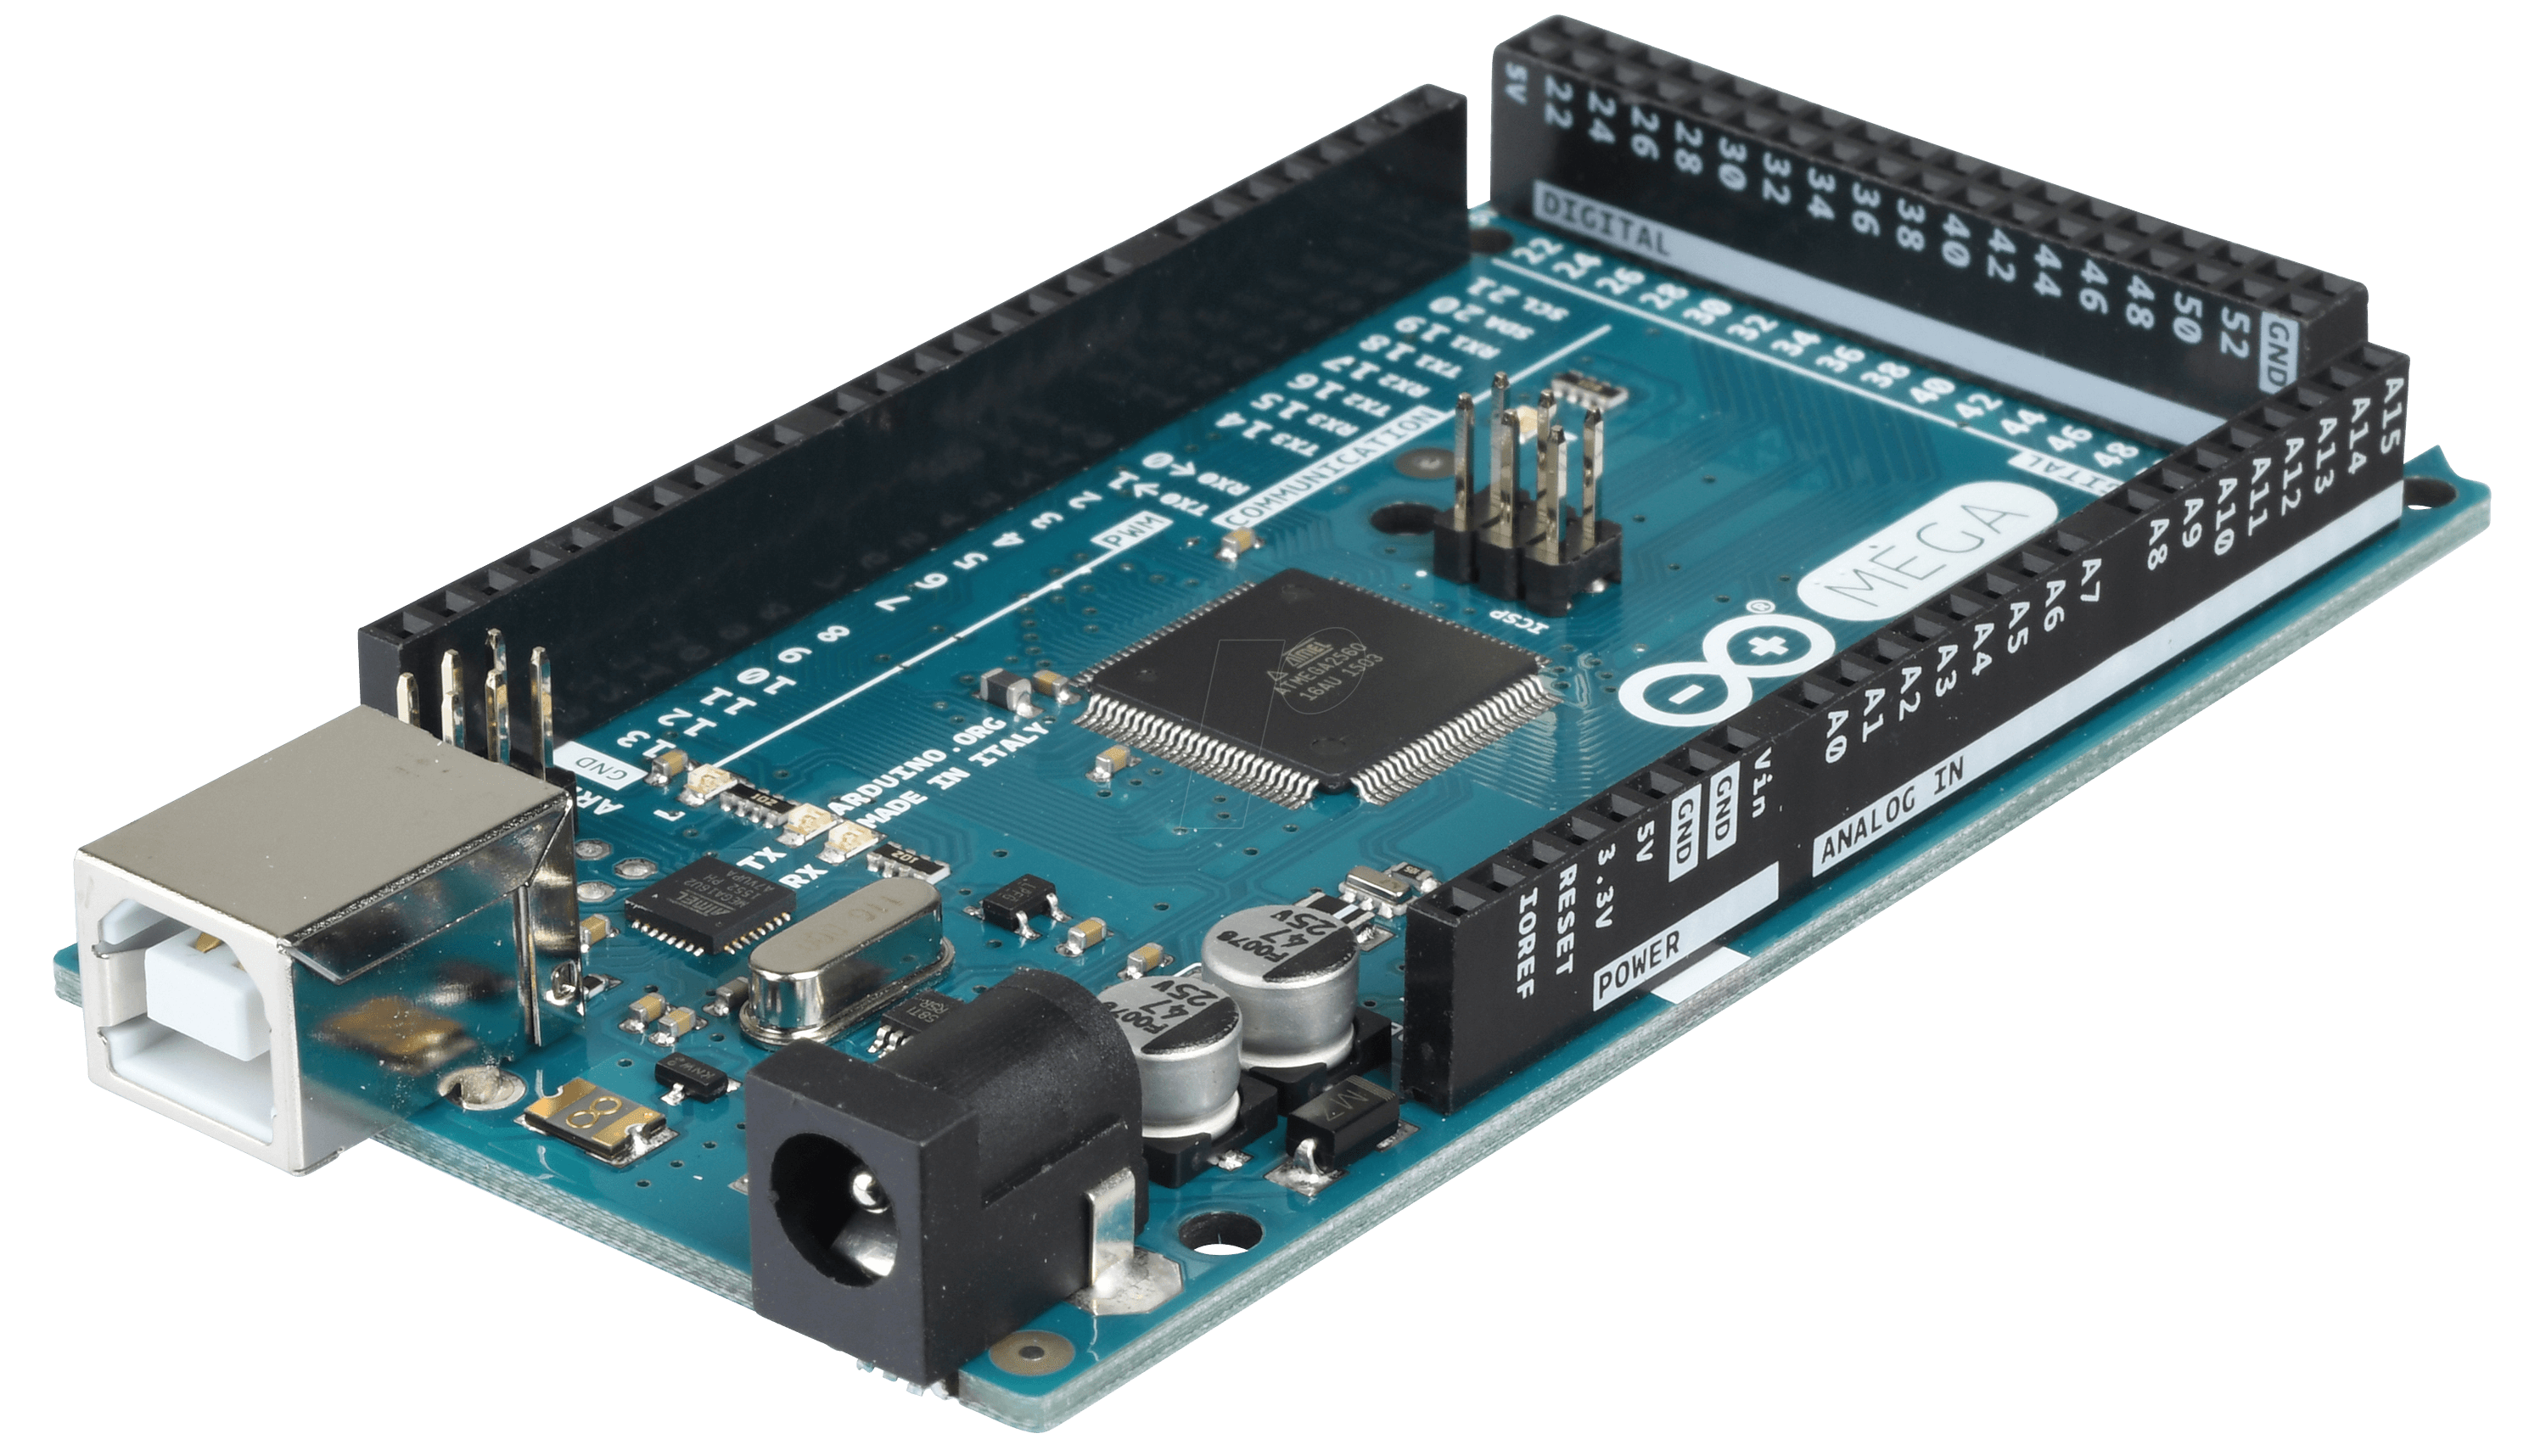
\includegraphics[trim = 0em 0em 0em 0em, clip, width=0.975\textwidth]{arduinoMega2560-iso.png}%
\caption[{[Selection of Compatible HW \& SW]: Arduino Mega 2560 (Isometric View)}]%
        {{[Selection of Compatible HW \& SW]: Arduino Mega 2560 (Isometric View)~%
           \cite{REF:online:reichelt:arduinoMega}%
           \label{FIG:preliminaryDecisions:selectionHardwareSoftware:hardware:components:microcontroller:iso}%
        }}%


\end{figure}

\vspace*{\fill}

\begin{figure}[H]%
\centering%
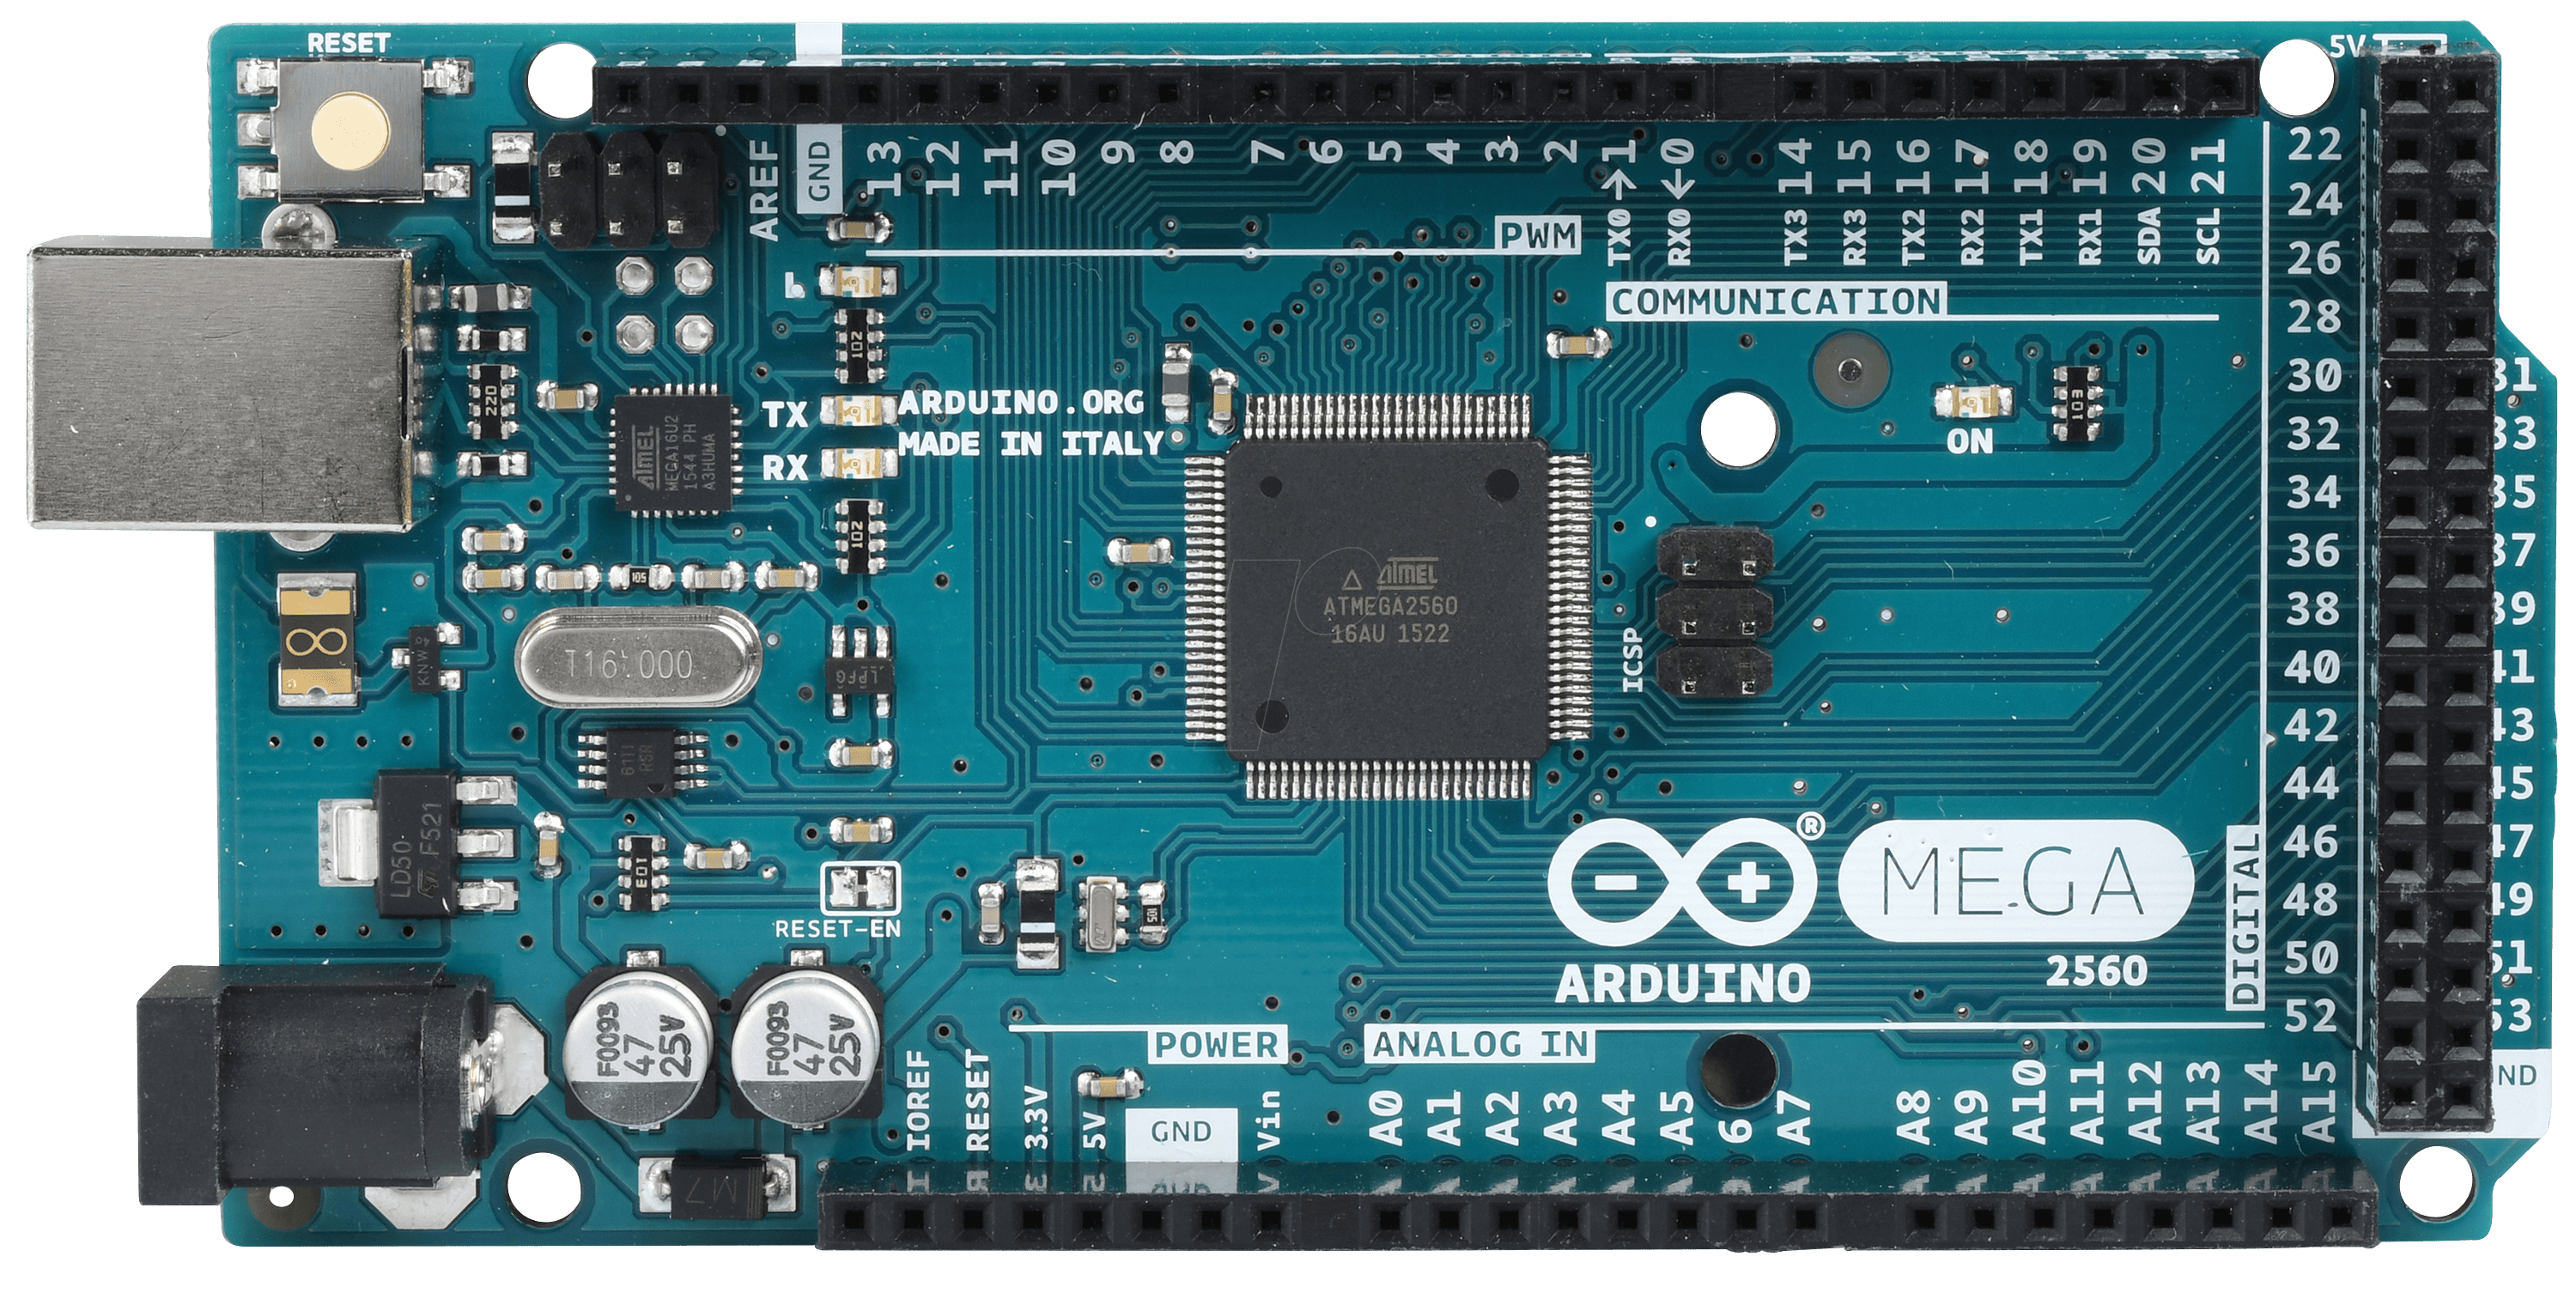
\includegraphics[trim = 0em 0em 0em 0em, clip, width=0.975\textwidth]{arduinoMega2560-top.png}%
\caption[{[Selection of Compatible HW \& SW]: Arduino Mega 2560 (Top View)}]%
        {{[Selection of Compatible HW \& SW]: Arduino Mega 2560 (Top View)~%
           \cite{REF:online:reichelt:arduinoMega}%
           \label{FIG:preliminaryDecisions:selectionHardwareSoftware:hardware:components:microcontroller:top}%
        }}%
\end{figure}

\vspace*{\fill}




\clearpage




\vspace*{\fill}
\begin{figure}[H]%
\centering%
\fbox{%
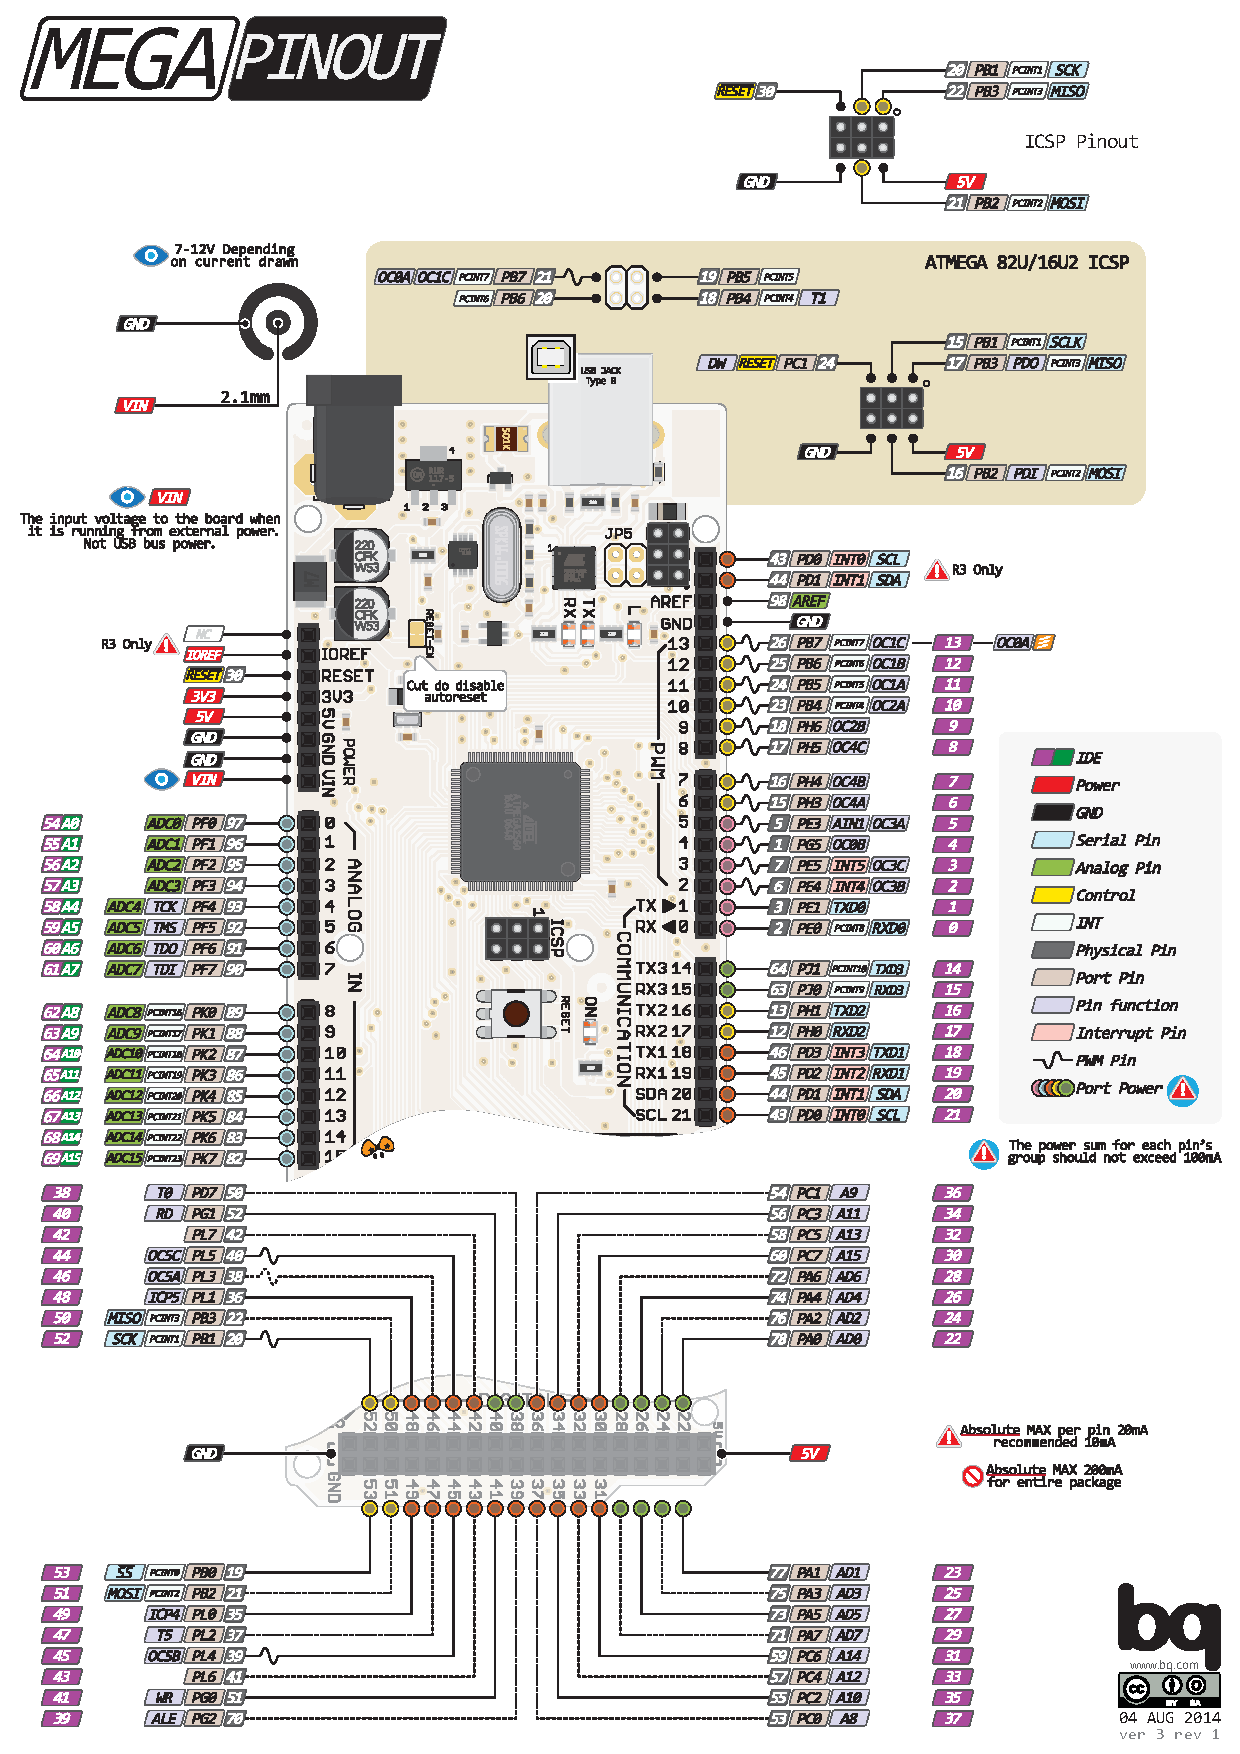
\includegraphics[trim = 0em 0em 0em 0em, clip, width=0.95\textwidth]{arduinoMega2560-pinout-v3p4.pdf}%
}%
\caption[{[Selection of Compatible HW \& SW]: Arduino Mega 2560 (Pin Map)}]%
        {{[Selection of Compatible HW \& SW]: Arduino Mega 2560 (Pin Map)~%
          \cite {REF:online:pighiXXX:pinout:arduinoMega}%
          \label{FIG:preliminaryDecisions:selectionHardwareSoftware:hardware:components:microcontroller:pin}%
        }}%
\end{figure}
\vspace*{\fill}




\clearpage



\iffalse

\subsubsubsectionA{Digital Outputs and PWM}




\subsubsubsectionA{Serial Controller}

-mention input buffer limits\\
-baud rate limits\\




\clearpage

\fi




\end{document}











% !TEX spellcheck = English (United States) (Aspell)
% !TEX TS-program = arara
%  arara: lmkclean
%  arara: pdflatex: {   draft: yes, options: '-file-line-error -halt-on-error' }
%  arara: biber
%  arara: pdflatex: {   draft: yes, options: '-file-line-error -halt-on-error' }
%  arara: pdflatex: { synctex: yes, options: '-file-line-error -halt-on-error' }
%  arara: lmkclean
\documentclass[crop=false,float=true,class=scrreprt]{standalone}

\providecommand{\main}{../../../../..}
% Preamble
 \input{\main/Subfiles/0-Preamble/1-packages.tex}

 \input{\main/Subfiles/0-Preamble/2-userInput-graphicsPath.tex}

 \input{\main/Subfiles/0-Preamble/3-pageLayout.tex}


% Watermark
 \input{\main/Subfiles/0-Preamble/watermark.tex}

% Floats:
 \input{\main/Subfiles/0-Preamble/floatConfig.tex}
%\input{\main/Subfiles/0-Preamble/sectionNumberIncludedInFloatCounter.tex}

% Commands:
 \input{\main/Subfiles/0-Preamble/commonCommands.tex}
 \input{\main/Subfiles/0-Preamble/allsubsSections.tex}
 \input{\main/Subfiles/0-Preamble/changePageSize.tex}

% Bug Fixes:
 \input{\main/Subfiles/0-Preamble/nociteFix.tex}
  % Preamble [document configuration]

\begin{document}


\iffalse

\subsubsection{Bluetooth Module}

-




\clearpage

\fi




\end{document}











% !TEX spellcheck = English (United States) (Aspell)
% !TEX TS-program = arara
%  arara: lmkclean
%  arara: pdflatex: {   draft: yes, options: '-file-line-error -halt-on-error' }
%  arara: biber
%  arara: pdflatex: {   draft: yes, options: '-file-line-error -halt-on-error' }
%  arara: pdflatex: { synctex: yes, options: '-file-line-error -halt-on-error' }
%  arara: lmkclean
\documentclass[crop=false,float=true,class=scrreprt]{standalone}

\providecommand{\main}{../../../../..}
% Preamble
 \input{\main/Subfiles/0-Preamble/1-packages.tex}

 \input{\main/Subfiles/0-Preamble/2-userInput-graphicsPath.tex}

 \input{\main/Subfiles/0-Preamble/3-pageLayout.tex}


% Watermark
 \input{\main/Subfiles/0-Preamble/watermark.tex}

% Floats:
 \input{\main/Subfiles/0-Preamble/floatConfig.tex}
%\input{\main/Subfiles/0-Preamble/sectionNumberIncludedInFloatCounter.tex}

% Commands:
 \input{\main/Subfiles/0-Preamble/commonCommands.tex}
 \input{\main/Subfiles/0-Preamble/allsubsSections.tex}
 \input{\main/Subfiles/0-Preamble/changePageSize.tex}

% Bug Fixes:
 \input{\main/Subfiles/0-Preamble/nociteFix.tex}
  % Preamble [document configuration]

\begin{document}


\subsubsection{Power Source}
\label{SEC:preliminaryDecisions:selectionHardwareSoftware:hardware:components:power}

The MinSeg M2V3 offers two independent sources of power:

\begin{itemize}[leftmargin=*, itemsep=-1.0em]
\item External power via a USB port
\item Internal power via an embedded battery holster
\end{itemize}

A physical switch exists on the MinSeg device to alternate between the two modes of power sourcing.




\subsubsubsectionA{External-Sourced Power (USB-Cable Connection)}

Externally-sourcing power via the USB port offers a constant 5 [V], per the USB standard;
however, the cable must be consistently connected to the robot body during use.




\subsubsubsectionA{Internal-Sourced Power (Battery Pack)}

As an alternative to externally-sourced power, 
power may be sourced from a battery holster embedded within the MinSeg.
The battery holster permits the installation of 6 AA-sized batteries.

A typical Alkaline AA-sized battery carries 1.5 [V] at maximum charge.
During use, this voltage will rapidly diminish to \raisebox{-0.75ex}{\textasciitilde}1.25 [V],
and more slowly diminish from then on to \raisebox{-0.75ex}{\textasciitilde}1.00 [V]
before rapidly becoming completely discharged, as depicted in Figure~%
\ref{FIG:preliminaryDecisions:selectionHardwareSoftware:hardware:components:power:batteryDrainage}.


\vspace*{+1.0em}
\begin{figure}[H]%
\small
\centering%
\fbox{%
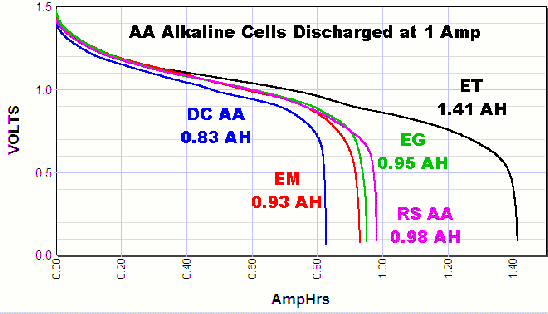
\includegraphics[trim = 0em 0.3em 0em 0em, clip, width=0.7\textwidth]{minseg-motor-batteryDrainage-1p0A.png}%
}%
\caption[{[Selection of Compatible HW \& SW]: AA-Battery Voltage During Constant Discharge}]%
        {{[Selection of Compatible HW \& SW]: AA-Battery Voltage During Constant Discharge~%
           \cite{REF:online:powerstream:batteryDrainage}%
           \label{FIG:preliminaryDecisions:selectionHardwareSoftware:hardware:components:power:batteryDrainage}%
        }}%
\end{figure}
\vspace*{-1.0em}


\iffalse%%%%%%%%%%%%%%%%%%%%
Note that a 0.5 A discharge was depicted in Figure~%
\ref{FIG:preliminaryDecisions:selectionHardwareSoftware:hardware:components:power:batteryDrainage}
since this is the approximate current of the motor during operation.
%https://www.modmypi.com/blog/how-do-i-power-my-arduino
%zhttp://playground.arduino.cc/Learning/WhatAdapter
This is depicted in Figure~%
\ref{FIG:preliminaryDecisions:selectionHardwareSoftware:hardware:components:power:motorCurrentVsLoadTorque}.


\vspace*{+1.0em}
\begin{figure}[H]%
\centering%
\fbox{%
\includegraphics[trim = 0em 0em 0em 0em, clip, width=0.7\textwidth]{minseg-motor-i-vs-T.gif}%
}%
\caption[{[Selection of Compatible HW \& SW]: Motor Current vs Load Torque}]%
        {{[Selection of Compatible HW \& SW]: Motor Current vs Load Torque~%
           \cite{REF:philohome}%
           \label{FIG:preliminaryDecisions:selectionHardwareSoftware:hardware:components:power:motorCurrentVsLoadTorque}%
        }}%
\end{figure}
\vspace*{-1.0em}
\fi%%%%%%%%%%%%%%%%%%%%%%%%%


To use the battery holster as a power source, all six AA batteries must be installed.
The batteries are connected in series and therefore cumulatively offer up to 9.00 [V] when at full charge.
During typical operation, the batteries will more likely offer a reduced voltage,
\raisebox{-0.75ex}{\textasciitilde}7.50 [V].

Therefore, sourcing power from the battery holster offers consistently greater voltage
than external USB-connected sources,
{\fns(\tif{so long as the batteries are not completely discharged})},
and additionally precludes the use of any wiring which could obstruct testing and operation.




\clearpage




\end{document}











% !TEX spellcheck = English (United States) (Aspell)
% !TEX TS-program = arara
%  arara: lmkclean
%  arara: pdflatex: {   draft: yes, options: '-file-line-error -halt-on-error' }
%  arara: biber
%  arara: pdflatex: {   draft: yes, options: '-file-line-error -halt-on-error' }
%  arara: pdflatex: { synctex: yes, options: '-file-line-error -halt-on-error' }
%  arara: lmkclean
\documentclass[crop=false,float=true,class=scrreprt]{standalone}

\providecommand{\main}{../../../../..}
% Preamble
 \input{\main/Subfiles/0-Preamble/1-packages.tex}

 \input{\main/Subfiles/0-Preamble/2-userInput-graphicsPath.tex}

 \input{\main/Subfiles/0-Preamble/3-pageLayout.tex}


% Watermark
 \input{\main/Subfiles/0-Preamble/watermark.tex}

% Floats:
 \input{\main/Subfiles/0-Preamble/floatConfig.tex}
%\input{\main/Subfiles/0-Preamble/sectionNumberIncludedInFloatCounter.tex}

% Commands:
 \input{\main/Subfiles/0-Preamble/commonCommands.tex}
 \input{\main/Subfiles/0-Preamble/allsubsSections.tex}
 \input{\main/Subfiles/0-Preamble/changePageSize.tex}

% Bug Fixes:
 \input{\main/Subfiles/0-Preamble/nociteFix.tex}
  % Preamble [document configuration]

\begin{document}


\subsubsection{Motor Driver}
\label{SEC:preliminaryDecisions:selectionHardwareSoftware:hardware:components:motorDriver}

The MinSeg M2V3 uses a Texas Instruments (TI) \tif{SN754410}: Quadruple Half-H Driver chip as a motor driver.
Supplementary information from the SN754410 datasheet is depicted in Figure~%
\ref{FIG:preliminaryDecisions:selectionHardwareSoftware:hardware:components:motorDriver:pinMap}
and Tables
\ref{TAB:preliminaryDecisions:selectionHardwareSoftware:hardware:components:motorDriver:pinLegend}~%
-~%
\ref{TAB:preliminaryDecisions:selectionHardwareSoftware:hardware:components:motorDriver:switchingCharacteristics}.

Figure~%
\ref{FIG:preliminaryDecisions:selectionHardwareSoftware:hardware:components:motorDriver:pinMap}
and Table~%
\ref{TAB:preliminaryDecisions:selectionHardwareSoftware:hardware:components:motorDriver:pinLegend}
exhibit that the chip has four inputs~$A$ and four corresponding outputs~$Y$.
Table~%
\ref{TAB:preliminaryDecisions:selectionHardwareSoftware:hardware:components:motorDriver:operatingConditions}
provides a simplified description of the behavior 
of any one input with respect to its corresponding output:

Input $A$ acts a switch for corresponding output $Y$:\\
\begin{tabular}{@{$\bullet$\ } l @{\ } c @{\ } c @{} l @{\ } c @{\ } l}
If the input pin $A$ is & enabled  & $V_{IH}$ &, then the corresponding output $Y$ will output & $V_{CC2}$ & $[V]$.\\[-0.0em]
If the input pin $A$ is & disabled & $V_{IL}$ &, then the corresponding output $Y$ will output & $0$       & $[V]$.
\end{tabular}\\[+0.5em]
{\fns \tif{Note}: It can be assumed that the enable $EN$ is engaged whenever necessary during MinSeg operation.}


\vspace*{\fill}


\begin{figure}[H]%
\centering%
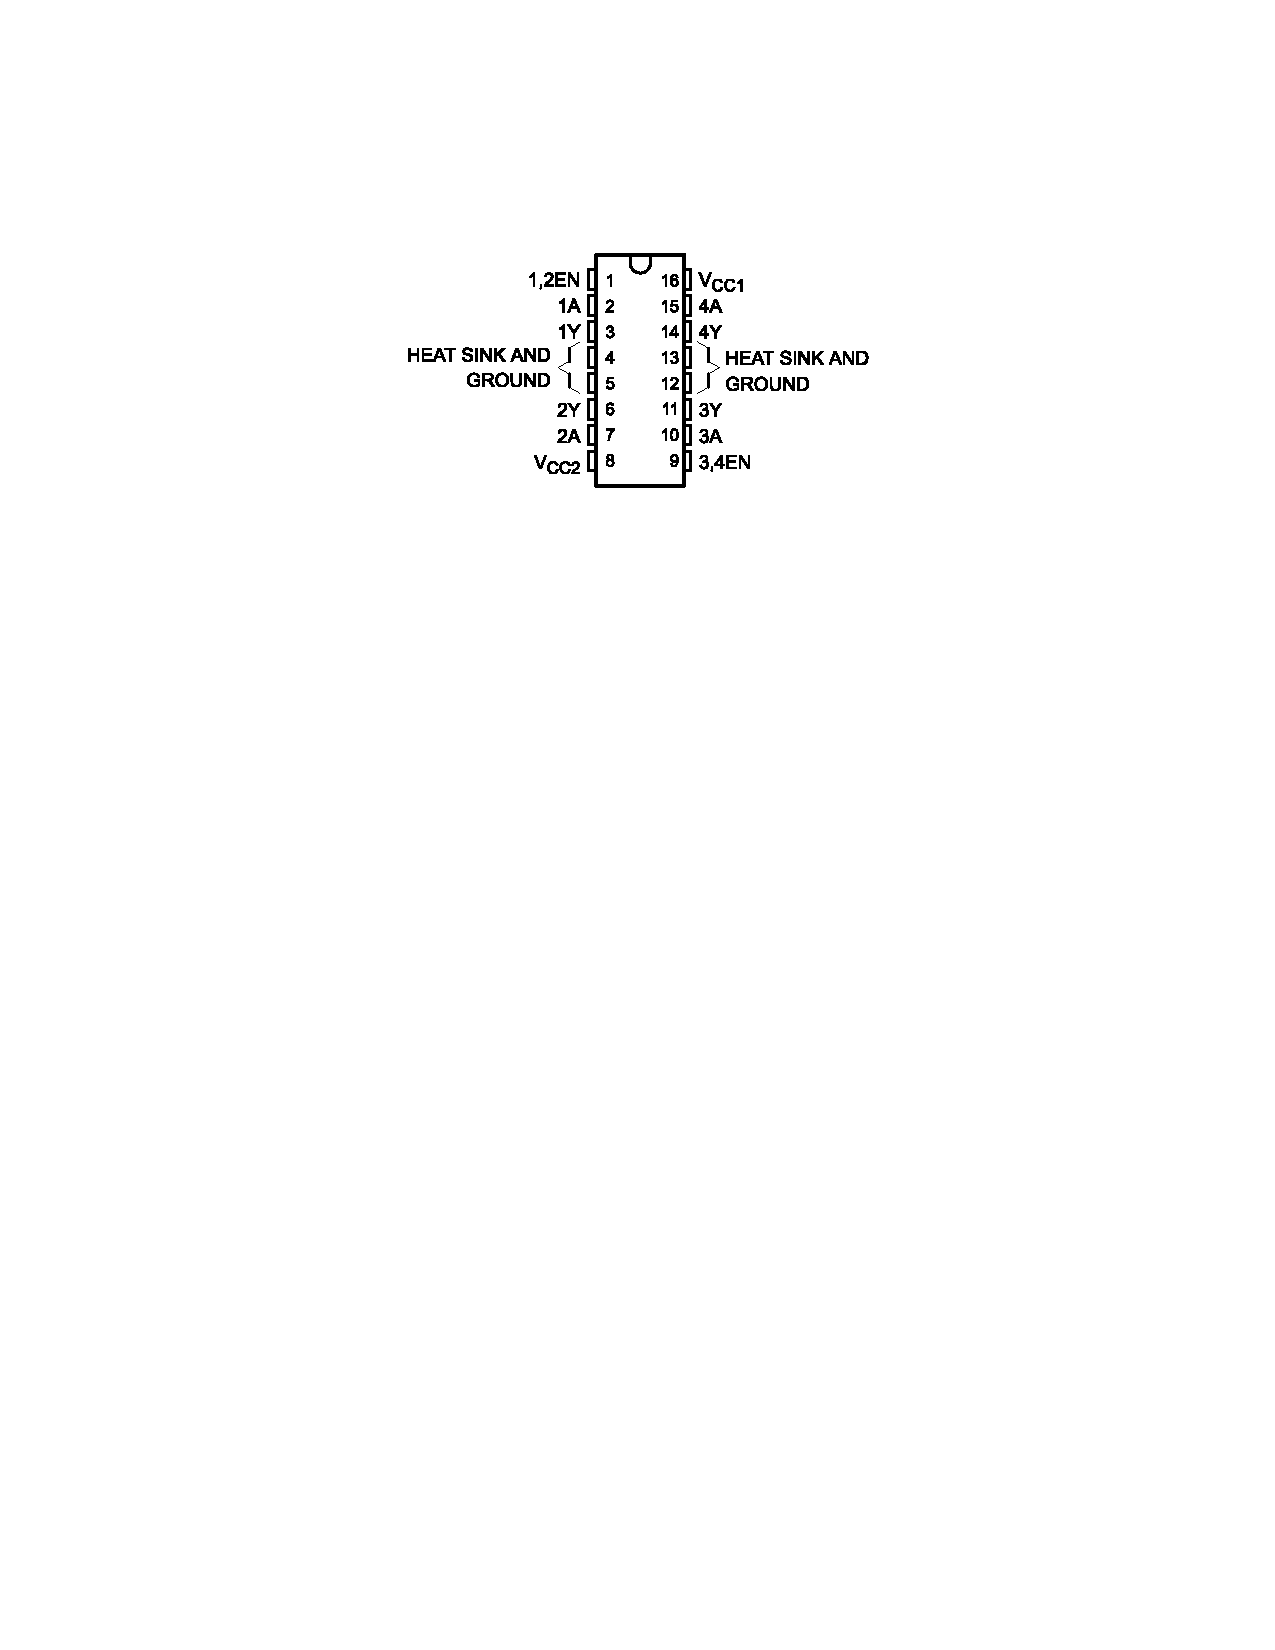
\includegraphics[trim = 0em 0em 0em 0em, clip, width=0.5\textwidth]{motor-driver-pinMap.pdf}%
\caption[{[Selection of Compatible HW \& SW]: Motor Driver Pin Map}]%
        {{[Selection of Compatible HW \& SW]: Motor Driver Pin Map~%
           \cite{REF:online:ti:datasheet:sn754410}%
           \label{FIG:preliminaryDecisions:selectionHardwareSoftware:hardware:components:motorDriver:pinMap}%
        }}%
\end{figure}


\vspace*{\fill}


\begin{table}[H]%
\centering%
\caption[{[Selection of Compatible HW \& SW]: Motor Driver Pin Legend}]%
        {{[Selection of Compatible HW \& SW]: Motor Driver Pin Legend~%
           \cite{REF:online:ti:datasheet:sn754410}%
           \label{TAB:preliminaryDecisions:selectionHardwareSoftware:hardware:components:motorDriver:pinLegend}%
        }}%
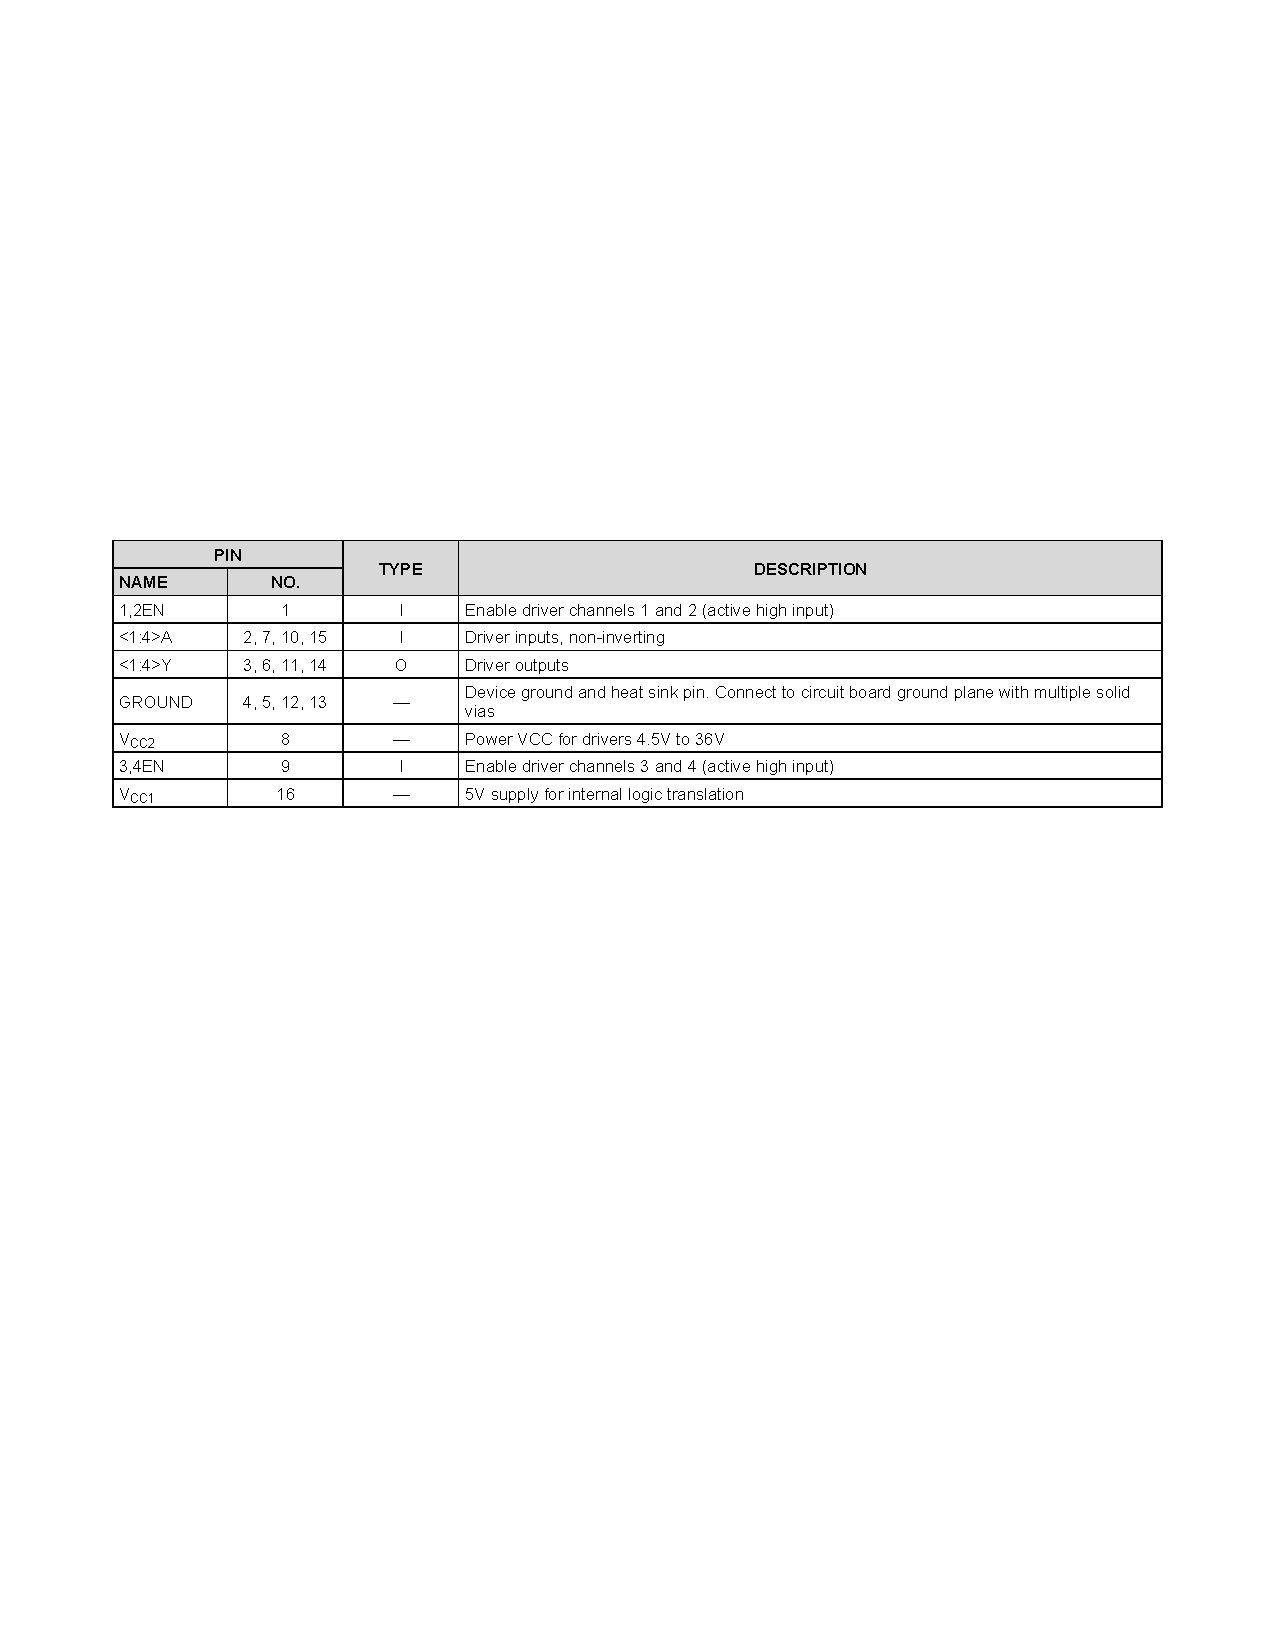
\includegraphics[trim = 0em 0em 0em 0em, clip, width=\textwidth]{motor-driver-pinLegend.pdf}%
\end{table}


\vspace*{\fill}




\clearpage





\vspace*{\fill}
\begin{table}[H]%
\centering%
\caption[{[Selection of Compatible HW \& SW]: Motor Driver Pin Function Legend}]%
        {{[Selection of Compatible HW \& SW]: Motor Driver Pin Function Legend~%
           \cite{REF:online:ti:datasheet:sn754410}%
           \label{TAB:preliminaryDecisions:selectionHardwareSoftware:hardware:components:motorDriver:pinFunctionLegend}%
        }}%
\vspace{+0.5em}
\begin{minipage}{\textwidth}%
\centering%
$\vcenter{\hbox{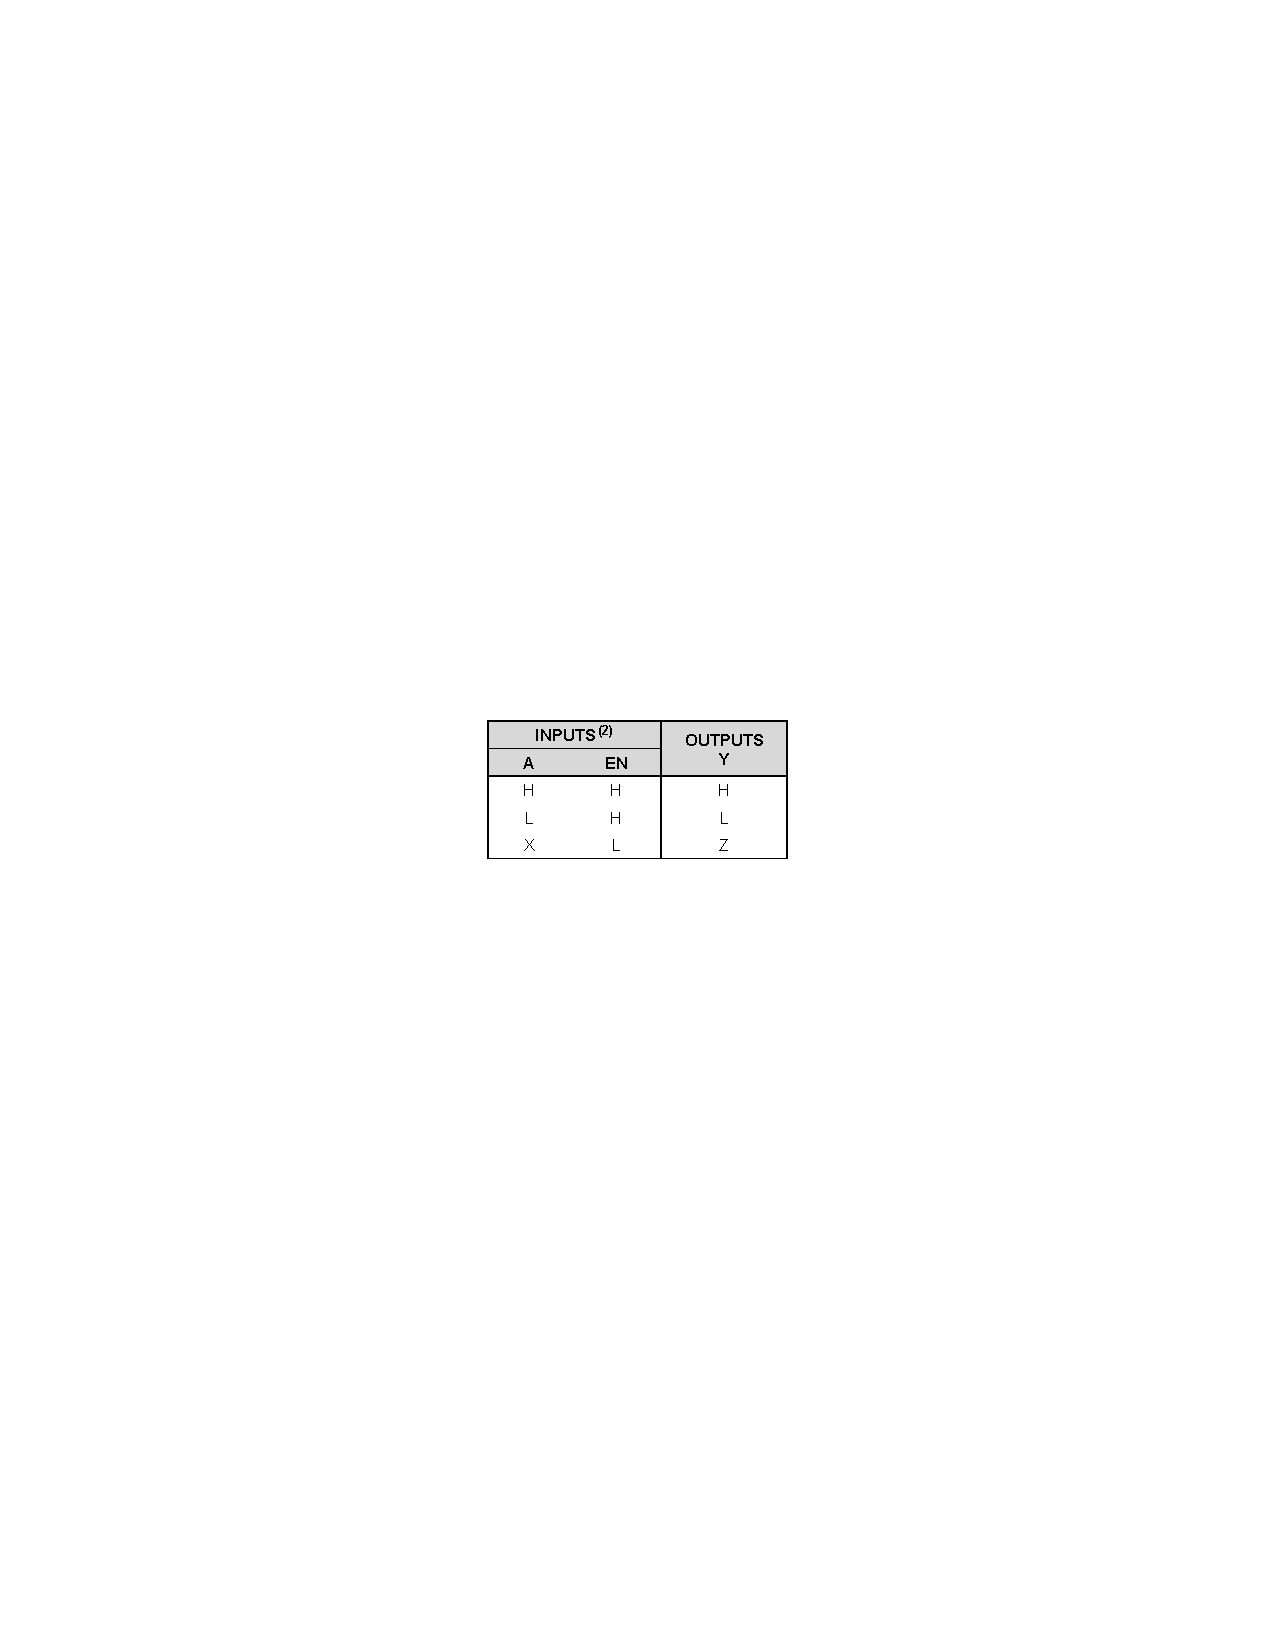
\includegraphics[trim = 0em 0em 0em 0em, clip, width=0.35\textwidth]{motor-driver-pinFunctionLegend1.pdf}}}$%
\hspace*{+2em}%
$\vcenter{\hbox{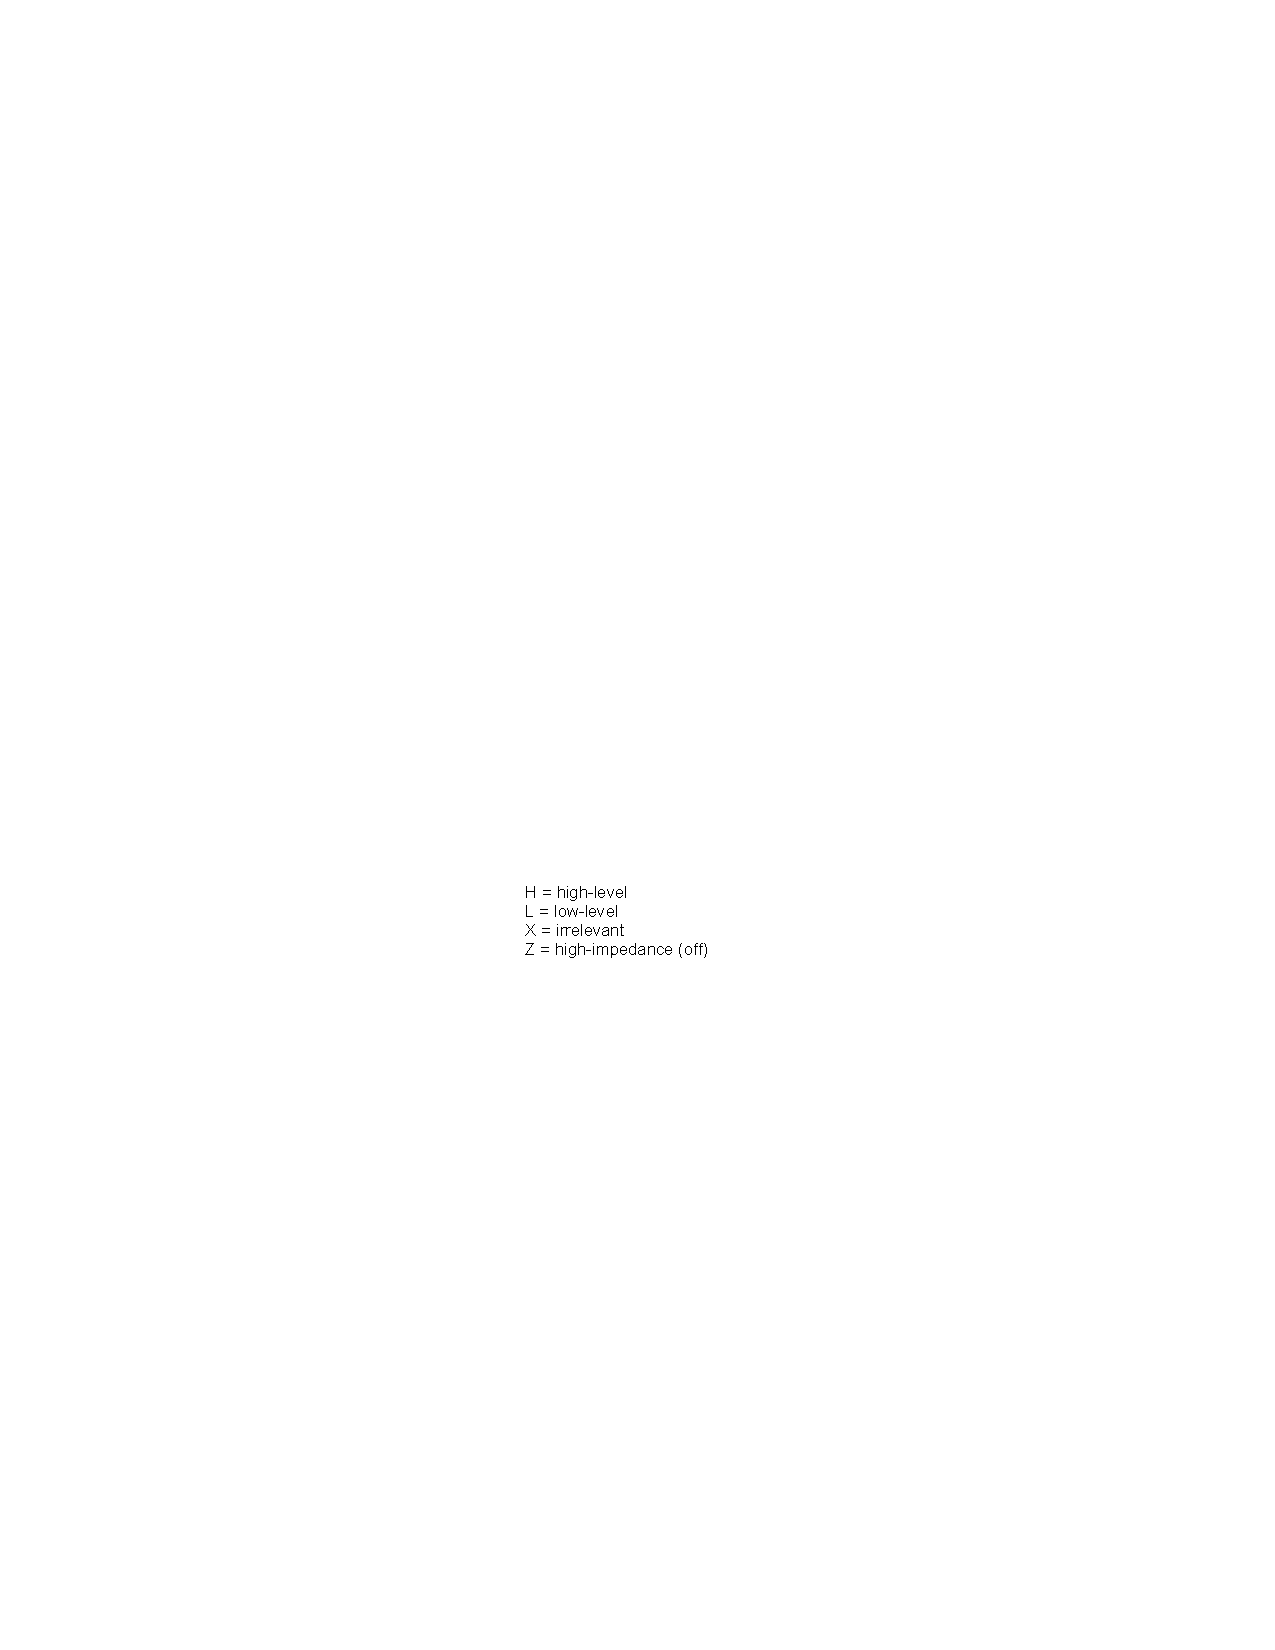
\includegraphics[trim = 0em 0em 0em 0em, clip, width=0.25\textwidth]{motor-driver-pinFunctionLegend2.pdf}}}$%
\end{minipage}%
\end{table}

\vspace*{\fill}

\begin{table}[H]%
\centering%
\caption[{[Selection of Compatible HW \& SW]: Motor Driver Operating Conditions}]%
        {{[Selection of Compatible HW \& SW]: Motor Driver Operating Conditions~%
           \cite{REF:online:ti:datasheet:sn754410}%
           \label{TAB:preliminaryDecisions:selectionHardwareSoftware:hardware:components:motorDriver:operatingConditions}%
        }}%
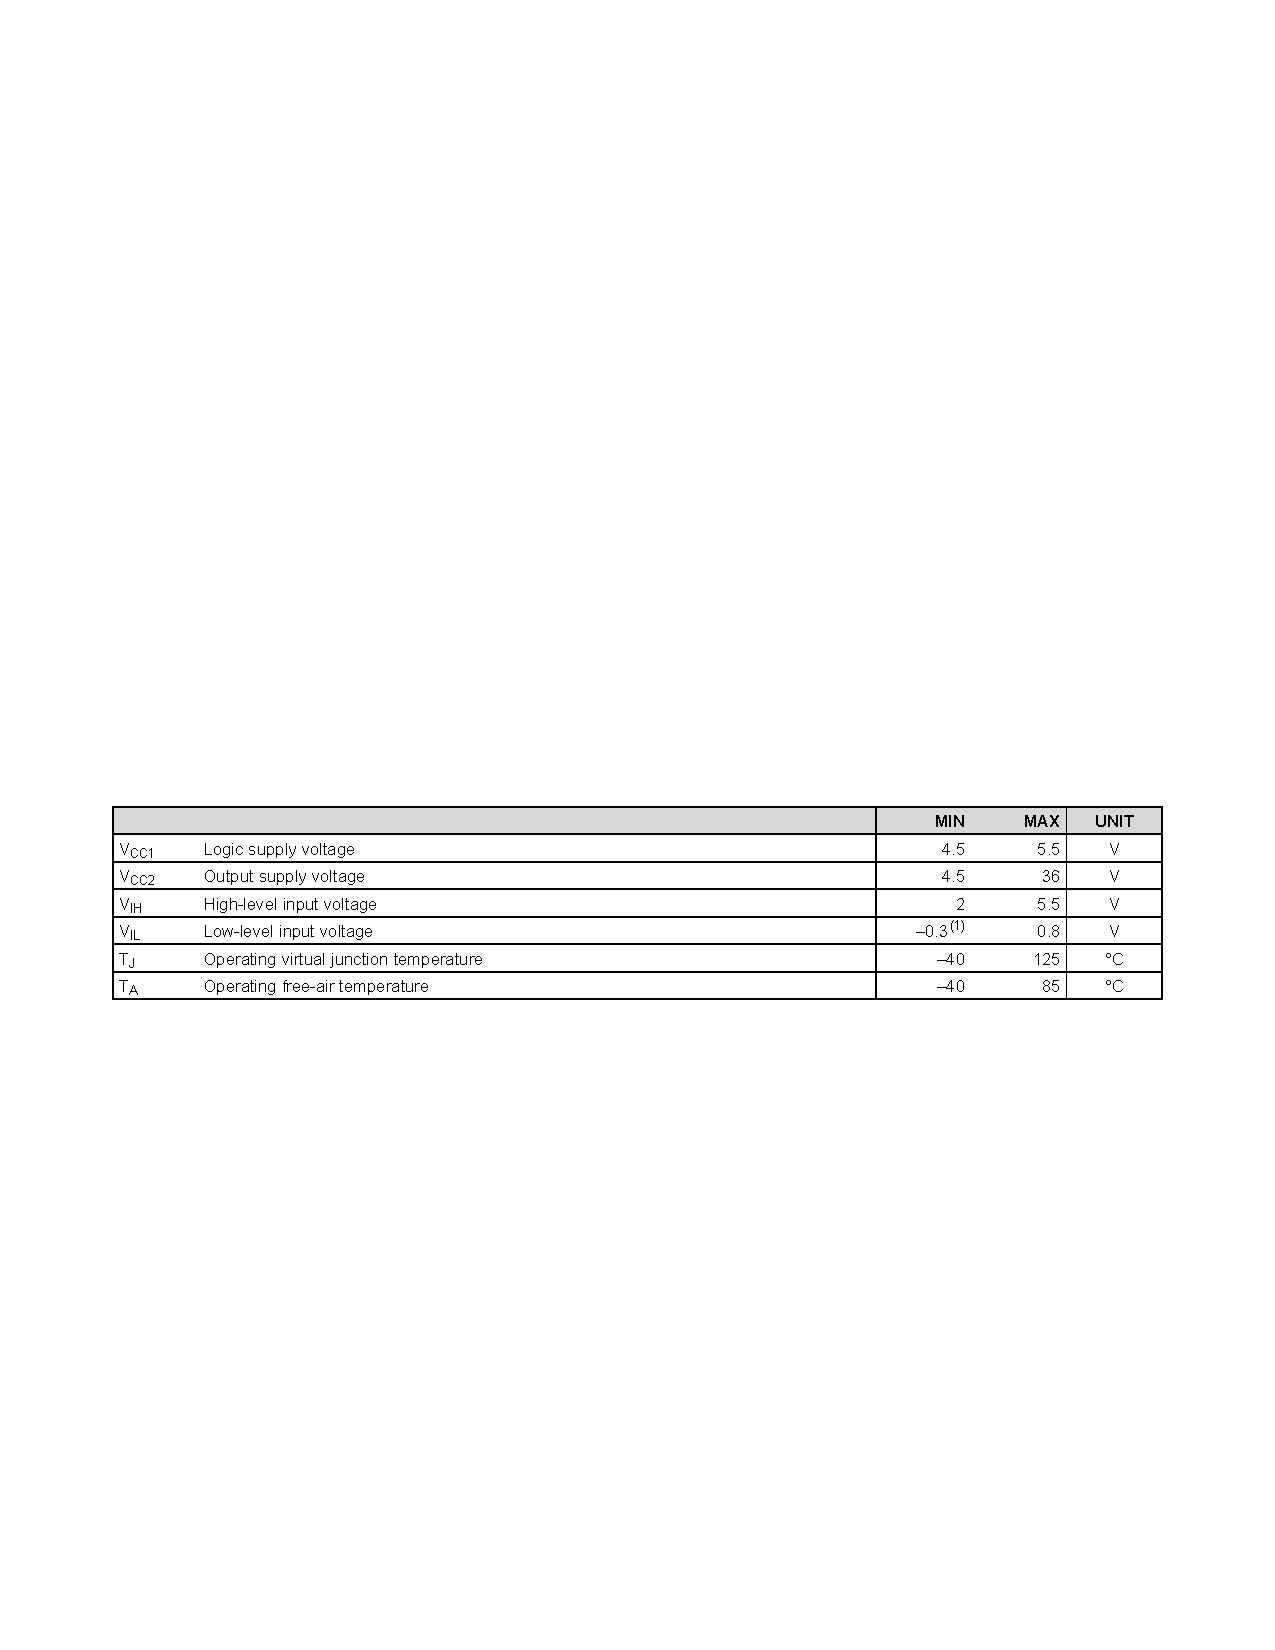
\includegraphics[trim = 0em 0em 0em 0em, clip, width=\textwidth]{motor-driver-operatingConditions.pdf}%
\end{table}

\vspace*{\fill}

\begin{table}[H]%
\centering%
\caption[{[Selection of Compatible HW \& SW]: Motor Driver Switching Characteristics}]%
        {{[Selection of Compatible HW \& SW]: Motor Driver Switching Characteristics~%
           \cite{REF:online:ti:datasheet:sn754410}%
           \label{TAB:preliminaryDecisions:selectionHardwareSoftware:hardware:components:motorDriver:switchingCharacteristics}%
        }}%
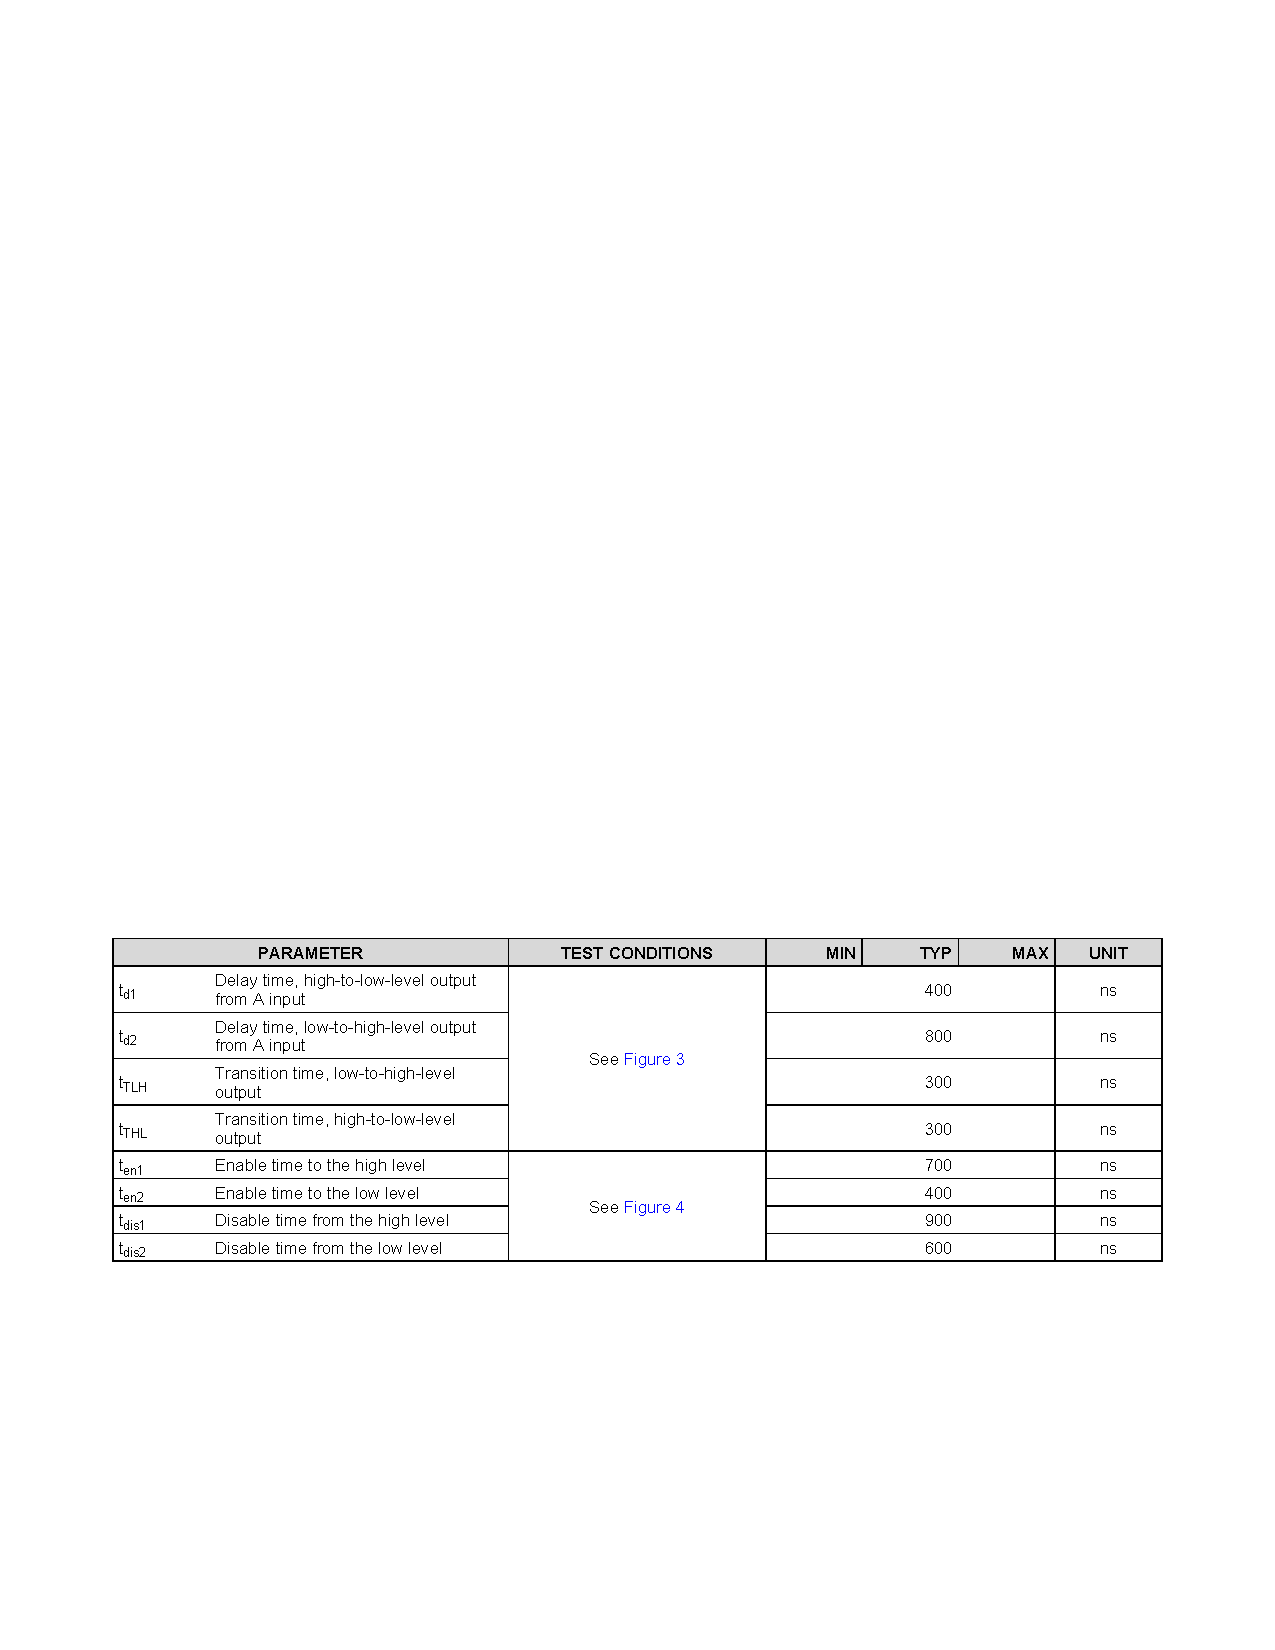
\includegraphics[trim = 0em 0em 0em 0em, clip, width=\textwidth]{motor-driver-switchingCharacteristics.pdf}%
\end{table}
\vspace*{\fill}




\clearpage




Table~%
\ref{TAB:preliminaryDecisions:selectionHardwareSoftware:hardware:components:motorDriver:operatingConditions}
specifies voltages associated with normal chip operation.
The voltage source for SN754410 outputs $V_{CC2}$ is wired to the MinSeg power source, 
and may therefore vary, from $4.5 - 9.0\ [V]$, {\fns(see Section~%
\ref{SEC:preliminaryDecisions:selectionHardwareSoftware:hardware:components:power}%
)}.

The SN754410 inputs $A$ are connected to digital output pins on the Arduino microcontroller, 
specifically those which are capable of producing pulse width modulated (PWM) signals
{\fns(see Sections~%
\ref{SEC:preliminaryDecisions:selectionHardwareSoftware:hardware:components:microcontroller}%
)}.
Programmed binary lows on the Arduino board will induce $0\ [V]$ 
and programmed binary highs will induce $5\ [V]$,
{\fns{(\tif{which is the Arduino board operating voltage})}}.


To achieve voltages other than $V_{CC2}$ exactly,
PWM voltage signals are used.
The Arduino can set its digital output pin to high
for a defined fraction of the time spanning
each sample interval of the Arduino board.
The effect of the added switching during each sample should be considered minimal,
since the MinSeg sample interval operates at the $10^{-3}\ [s]$ scale
{\fns(\tif{as set by the operator})},
and the SN754410 switching interval operates at the $10^{-7}\ [s]$ scale,
{\fns(\tif{per Table~%
\ref{TAB:preliminaryDecisions:selectionHardwareSoftware:hardware:components:motorDriver:switchingCharacteristics}%
})}.

As stated in Section~%
\ref{SEC:preliminaryDecisions:selectionHardwareSoftware:hardware:components},
there are two DC motors.  
Each has a positive and negative lead.




\clearpage




\end{document}











% !TEX spellcheck = English (United States) (Aspell)
% !TEX TS-program = arara
%  arara: lmkclean
%  arara: pdflatex: {   draft: yes, options: '-file-line-error -halt-on-error' }
%  arara: biber
%  arara: pdflatex: {   draft: yes, options: '-file-line-error -halt-on-error' }
%  arara: pdflatex: { synctex: yes, options: '-file-line-error -halt-on-error' }
%  arara: lmkclean
\documentclass[crop=false,float=true,class=scrreprt]{standalone}

\providecommand{\main}{../../../../..}
% Preamble
 \input{\main/Subfiles/0-Preamble/1-packages.tex}

 \input{\main/Subfiles/0-Preamble/2-userInput-graphicsPath.tex}

 \input{\main/Subfiles/0-Preamble/3-pageLayout.tex}


% Watermark
 \input{\main/Subfiles/0-Preamble/watermark.tex}

% Floats:
 \input{\main/Subfiles/0-Preamble/floatConfig.tex}
%\input{\main/Subfiles/0-Preamble/sectionNumberIncludedInFloatCounter.tex}

% Commands:
 \input{\main/Subfiles/0-Preamble/commonCommands.tex}
 \input{\main/Subfiles/0-Preamble/allsubsSections.tex}
 \input{\main/Subfiles/0-Preamble/changePageSize.tex}

% Bug Fixes:
 \input{\main/Subfiles/0-Preamble/nociteFix.tex}
  % Preamble [document configuration]

\begin{document}

\subsubsection{Motor, Gearbox, and Encoder}
\label{SEC:preliminaryDecisions:selectionHardwareSoftware:hardware:components:motor}

The MinSeg implements two Lego NXT servo motors.
Each Lego NXT servo motor contains a DC traction motor, a gearbox, and an encoder.
A three-dimensional model of the component is depicted in Figure~%
\ref{FIG:preliminaryDecisions:selectionHardwareSoftware:hardware:components:motor:3d}.

\vspace*{+1.0em}
\begin{figure}[H]%
\centering%
\fbox{%
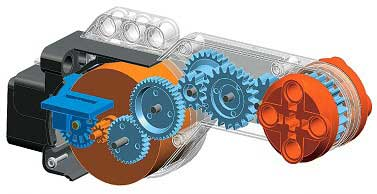
\includegraphics[trim = 0em 0em 0em 0em, clip, width=0.55\textwidth]{minseg-motor-3d.jpg}%
}%
\caption[{[Selection of Compatible HW \& SW]: Lego NXT Motor (3D Model)}]%
        {{[Selection of Compatible HW \& SW]: Lego NXT Motor (3D Model)~%
           \cite{REF:online:philohome}%
           \label{FIG:preliminaryDecisions:selectionHardwareSoftware:hardware:components:motor:3d}%
        }}%
\end{figure}
\vspace*{-1.0em}

Although Lego did not publicly disclose all of the characteristic parameters of their components,
the hobbyist community reverse engineered several of these values by performing various tests
and also by (irreversibly) dismantling a spare~%
\cite{REF:online:philohome}.
The dismantled component is depicted in Figure~%
\ref{FIG:preliminaryDecisions:selectionHardwareSoftware:hardware:components:motor:exploded}.


\vspace*{+1.0em}
\begin{figure}[H]%
\centering%
\fbox{%
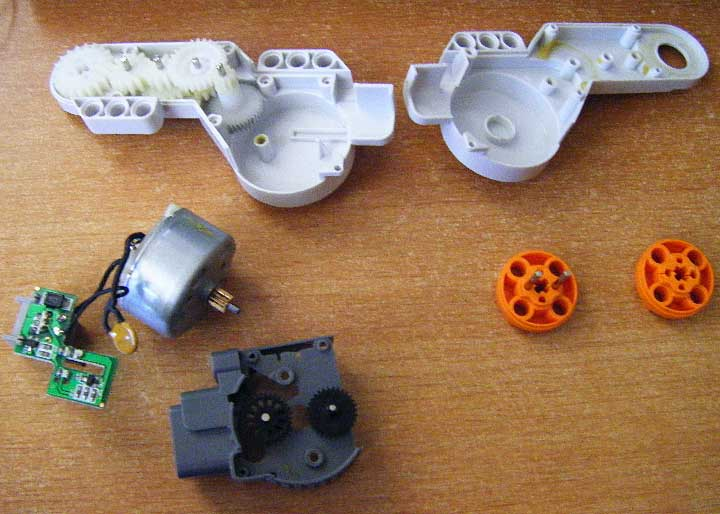
\includegraphics[trim = 0em 0em 0em 0em, clip, width=0.8\textwidth]{minseg-motor-exploded.jpg}%
}%
\caption[{[Selection of Compatible HW \& SW]: Lego NXT Motor (Exploded)}]%
        {{[Selection of Compatible HW \& SW]: Lego NXT Motor (Exploded)~%
           \cite{REF:online:philohome}%
           \label{FIG:preliminaryDecisions:selectionHardwareSoftware:hardware:components:motor:exploded}%
           }}%
\end{figure}
\vspace*{-1.0em}




\clearpage




Table~%
\ref{TAB:preliminaryDecisions:selectionHardwareSoftware:hardware:components:motor:figureLegend}
provides a legend for the different components in Figures
\ref{FIG:preliminaryDecisions:selectionHardwareSoftware:hardware:components:motor:3d}~%
-~%
\ref{FIG:preliminaryDecisions:selectionHardwareSoftware:hardware:components:motor:exploded}.

\vspace*{+0.0em}
\begin{table}[H]%
\centering%
\small%
\caption[{[Selection of Compatible HW \& SW]: Lego NXT Motor Figure Legend}]%
        {{[Selection of Compatible HW \& SW]: Lego NXT Motor Figure Legend~%
           \cite{REF:online:philohome}%
           \label{TAB:preliminaryDecisions:selectionHardwareSoftware:hardware:components:motor:figureLegend}%
           }}
\vspace{+0.25em}
\begin{tabular}{| l | c | c | c |}                                                                                  \hline     \\[-2.0em]
\mc{1}{|c|}{%
\tbf{Component}%
}                                                                                                        &
\tbf{Figure \ref{FIG:preliminaryDecisions:selectionHardwareSoftware:hardware:components:motor:3d}}       &
\mc{2}{c |}{%
\tbf{Figure \ref{FIG:preliminaryDecisions:selectionHardwareSoftware:hardware:components:motor:exploded}}% 
}                                                                                                        \\[+0.0em] \hline &&& \\[-2.0em]
%%
Enclosure                                                                                                &
\begin{tabular}{@{}l@{}}
Translucent                       \\
\end{tabular}                                                                                            &
\begin{tabular}{@{}c@{}}
Top                               \\
\end{tabular}                                                                                            &
\begin{tabular}{@{}c@{}}
Grey                              \\
\end{tabular}                                                                                            \\[+0.0em] \hline &&& \\[-2.0em]
%%
\begin{tabular}{@{}l@{}}
Encoder                           \\
\tif{\ \ Enclosure}               \\
\tif{\ \ Gearing}
\end{tabular}                                                                                            &
\begin{tabular}{@{}c@{}}
-                                 \\
Dark blue                         \\
Dark grey                         \\
\end{tabular}                                                                                            &
\begin{tabular}{@{}c@{}}
-                                 \\
Bottom                            \\
Bottom                            \\
\end{tabular}                                                                                            &
\begin{tabular}{@{}c@{}}
-                                 \\
Black                             \\
Dark grey                         \\
\end{tabular}                                                                                            \\[+0.0em] \hline &&& \\[-2.0em]
%%
PCB                                                                                                      & 
\begin{tabular}{@{}c@{}}
-                                 \\
\end{tabular}                                                                                            &
\begin{tabular}{@{}c@{}}
Left                              \\
\end{tabular}                                                                                            &
\begin{tabular}{@{}c@{}}
Green                             \\
\end{tabular}                                                                                            \\[+0.0em] \hline &&& \\[-2.0em]
%%
Motor                                                                                                    & 
\begin{tabular}{@{}c@{}}
Light orange                      \\
\end{tabular}                                                                                            &
\begin{tabular}{@{}c@{}}
Left                              \\
\end{tabular}                                                                                            &
\begin{tabular}{@{}c@{}}
Chrome                            \\
\end{tabular}                                                                                            \\[+0.0em] \hline &&& \\[-2.0em]
%%
Gearbox                                                                                                  & 
\begin{tabular}{@{}c@{}}
Light blue                        \\
\end{tabular}                                                                                            &
\begin{tabular}{@{}c@{}}
Top-Left                          \\
\end{tabular}                                                                                            &
\begin{tabular}{@{}c@{}}
White                             \\
\end{tabular}                                                                                            \\[+0.0em] \hline &&& \\[-2.0em]
%%
Wheel axle mount                                                                                         & 
\begin{tabular}{@{}c@{}}
Dark orange                       \\
\end{tabular}                                                                                            &
\begin{tabular}{@{}c@{}}
Right                             \\
\end{tabular}                                                                                            &
\begin{tabular}{@{}c@{}}
Orange                            \\
\end{tabular}                                                                                            \\[+0.0em] \hline
%%
\end{tabular}
\end{table}
\vspace*{-1.0em}





\subsubsubsectionA{Gearing}

The encoder, the motor, and the wheel axle mount
are coupled through gearing.
Thus, the angular velocity $\omega$ of any one of these components 
can be related to 
the angular velocity of any one of the other components
based on the the number(s) of teeth between each component,
as exhibited in Eqn.~%
[\ref{EQN:preliminaryDecisions:selectionHardwareSoftware:hardware:components:motor:gearTeeth}],
where $k$ represents a ratio and $n$ represents an integer count.

\begin{equation}
\label{EQN:preliminaryDecisions:selectionHardwareSoftware:hardware:components:motor:gearTeeth}
k_{\omega\ A2B}
=
\frac{n_{\omega\ B}}{n_{\omega\ A}}
=
\begin{bmatrix}
\displaystyle
k_{teeth\ A2B}
\end{bmatrix}^{-1}
=
\begin{bmatrix}
\displaystyle
\frac{n_{teeth\ B}}{n_{teeth\ A}}
\end{bmatrix}^{-1}
\end{equation}


The number of teeth in each gearing is depicted in Figure~%
\ref{FIG:preliminaryDecisions:selectionHardwareSoftware:hardware:components:motor:gearTeethMap}.
Teeth counts in the same row are coupled by teeth.  
Teeth counts in the same column are coupled by axle,
{\fns(\tif{and therefore rotate at the same rate, independent of teeth count})}.


\vspace*{\fill}
\begin{figure}[H]
\setcounter{MaxMatrixCols}{20}
\centering%
\fbox{%
$%
\begin{matrix}%
20    & | & 13    & 10    & \cdot & \cdot & \cdot & | & \cdot & | & \cdot \\
\cdot & | & \cdot & 20    & 10    & \cdot & \cdot & | & \cdot & | & \cdot \\
\cdot & | & \cdot & \cdot & 27    & 09    & \cdot & | & \cdot & | & \cdot \\
\cdot & | & \cdot & \cdot & \cdot & 40    & 30    & | & 10    & | & 32    \\
\end{matrix}%
$%
}%
\caption[{[Selection of Compatible HW \& SW]: Lego NXT Motor Gear Teeth Map}]%
        {{[Selection of Compatible HW \& SW]: Lego NXT Motor Gear Teeth Map~%
           \cite{REF:online:philohome}%
           \label{FIG:preliminaryDecisions:selectionHardwareSoftware:hardware:components:motor:gearTeethMap}%
           }}%
\end{figure}
\vspace*{\fill}




\clearpage




Additionally, in Figure~%
\ref{FIG:preliminaryDecisions:selectionHardwareSoftware:hardware:components:motor:gearTeethMap},
each component is separated by a vertical bar.
From left to right: wheel axle mount, gearbox, motor, encoder.
The completed relation between the wheel axle mount and the gearbox is exhibited in Eqns.
[\ref{EQN:preliminaryDecisions:selectionHardwareSoftware:hardware:components:motor:gearTeeth:finalValue1}~%
--%
\ref{EQN:preliminaryDecisions:selectionHardwareSoftware:hardware:components:motor:gearTeeth:finalValue6}].


\begin{align}
\label{EQN:preliminaryDecisions:selectionHardwareSoftware:hardware:components:motor:gearTeeth:finalValue1}
%%
k_{gearTeeth\ wheel2motor}
&=&
\begin{bmatrix} \displaystyle
\frac{13}{20} \cdot\frac{10}{13}
\end{bmatrix}
\cdot %%%%%%
\begin{bmatrix} \displaystyle
\frac{10}{20}
\end{bmatrix}
\cdot %%%%%%
\begin{bmatrix} \displaystyle
\frac{09}{27}
\end{bmatrix}
\cdot %%%%%%
\begin{bmatrix} \displaystyle
\frac{30}{40} \cdot\frac{10}{30}
\end{bmatrix}
=
\frac{01}{48}
%%
%%
\\[+2em]
%%
%%
k_{gearTeeth\ motor2encoder}
&=&
\frac{32}{10}
%%
%%
\\[+2em]
%%
%%
k_{\omega\ wheel2motor}
&=&
\begin{bmatrix} \displaystyle
k_{gearTeeth\ wheel2motor}
\end{bmatrix}^{-1}
=
\frac{48}{01}
%%
%%
\\[+2em]
%%
%%
k_{\omega \ motor2encoder}
&=&
\begin{bmatrix} \displaystyle
k_{gearTeeth\ motor2encoder}
\end{bmatrix}^{-1}
=
\frac{10}{32}
%%
%%
\\[+2em]
%%
%%
\label{EQN:preliminaryDecisions:selectionHardwareSoftware:hardware:components:motor:gearTeeth:finalValue6}
k_{\omega\ wheel2encoder}
&=&
k_{\omega\ wheel2motor}
\cdot
k_{\omega\ motor2encoder}
=
\frac{15}{01}
%%
\end{align}




\iffalse

\subsubsubsectionA{Motor}

motor torque constant\\
motor back emf constant\\


\subsubsubsectionA{Encoder}

slots\\
binary\\
quadrature\\

\fi





\clearpage




\end{document}











% !TEX spellcheck = English (United States) (Aspell)
% !TEX TS-program = arara
%  arara: lmkclean
%  arara: pdflatex: {   draft: yes, options: '-file-line-error -halt-on-error' }
%  arara: biber
%  arara: pdflatex: {   draft: yes, options: '-file-line-error -halt-on-error' }
%  arara: pdflatex: { synctex: yes, options: '-file-line-error -halt-on-error' }
%  arara: lmkclean
\documentclass[crop=false,float=true,class=scrreprt]{standalone}

\providecommand{\main}{../../../../..}
% Preamble
 \input{\main/Subfiles/0-Preamble/1-packages.tex}

 \input{\main/Subfiles/0-Preamble/2-userInput-graphicsPath.tex}

 \input{\main/Subfiles/0-Preamble/3-pageLayout.tex}


% Watermark
 \input{\main/Subfiles/0-Preamble/watermark.tex}

% Floats:
 \input{\main/Subfiles/0-Preamble/floatConfig.tex}
%\input{\main/Subfiles/0-Preamble/sectionNumberIncludedInFloatCounter.tex}

% Commands:
 \input{\main/Subfiles/0-Preamble/commonCommands.tex}
 \input{\main/Subfiles/0-Preamble/allsubsSections.tex}
 \input{\main/Subfiles/0-Preamble/changePageSize.tex}

% Bug Fixes:
 \input{\main/Subfiles/0-Preamble/nociteFix.tex}
  % Preamble [document configuration]

\begin{document}


\iffalse

\subsubsection{Gyroscope and Accelerometer}
\label{SEC:preliminaryDecisions:selectionHardwareSoftware:hardware:components:gyroAccel}

precision (250 deg/s)\\
bias\\

figure of axes\\




\clearpage

\fi




\end{document}











% !TEX spellcheck = English (United States) (Aspell)
% !TEX TS-program = arara
%  arara: lmkclean
%  arara: pdflatex: {   draft: yes, options: '-file-line-error -halt-on-error' }
%  arara: biber
%  arara: pdflatex: {   draft: yes, options: '-file-line-error -halt-on-error' }
%  arara: pdflatex: { synctex: yes, options: '-file-line-error -halt-on-error' }
%  arara: lmkclean
\documentclass[crop=false,float=true,class=scrreprt]{standalone}

\providecommand{\main}{../../../../..}
% Preamble
 \input{\main/Subfiles/0-Preamble/1-packages.tex}

 \input{\main/Subfiles/0-Preamble/2-userInput-graphicsPath.tex}

 \input{\main/Subfiles/0-Preamble/3-pageLayout.tex}


% Watermark
 \input{\main/Subfiles/0-Preamble/watermark.tex}

% Floats:
 \input{\main/Subfiles/0-Preamble/floatConfig.tex}
%\input{\main/Subfiles/0-Preamble/sectionNumberIncludedInFloatCounter.tex}

% Commands:
 \input{\main/Subfiles/0-Preamble/commonCommands.tex}
 \input{\main/Subfiles/0-Preamble/allsubsSections.tex}
 \input{\main/Subfiles/0-Preamble/changePageSize.tex}

% Bug Fixes:
 \input{\main/Subfiles/0-Preamble/nociteFix.tex}
  % Preamble [document configuration]

\begin{document}


\iffalse

\subsubsection{Arduino Interfaces}
\label{SEC:preliminaryDecisions:selectionHardwareSoftware:hardware:components:interfaces}

board sample rate\\
board run time (inf)\\

serial to/from board\\
maximize serial speed\\


Due to the inclusion of a USB port, interfacing with the board is relatively convenient,
whether for programming the board 
or for data transmission during operation.
Additionally, due to the inclusion of multiple UARTs, 
the board can be configured 


-power (see previous section)
-communication: serial (usb or bluetooth)
-wired or wireless



This can be beneficial when the USB connection is already being used to perform communication;
for example, during microcontroller programming 
or during operation for wired data transmission..

During microcontroller programming, this is especially ideal 
since the location and, particularly, the attitude of the robot is not significant.

Contrarily, during operation,
the robot will need to consistently balance at or near an upright position.
While the mass from the cable may be relatively insignificant,
tension in the cable could induce significant disturbance forces on the robot
during trajectory.
These disturbances are beyond the scope of the planned studies,
and therefore will be avoided during testing.

\fi


\clearpage




\end{document}















%\renewcommand{\sectionedEquation}{\thesection--\arabic{equation}}
%\counterwithout*{equation}{subsection}

%\stopcontents[preliminaryDecisions:selectionHardware]
%\addtocontents{toc}{\string\setcounter{tocdepth}{1}}



\end{document}











% !TEX spellcheck = English (United States) (Aspell)
% !TEX TS-program = arara
%  arara: lmkclean
%  arara: pdflatex: {   draft: yes, options: '-file-line-error -halt-on-error' }
%  arara: biber
%  arara: pdflatex: {   draft: yes, options: '-file-line-error -halt-on-error' }
%  arara: pdflatex: { synctex: yes, options: '-file-line-error -halt-on-error' }
%  arara: lmkclean
\documentclass[crop=false,float=true,class=scrreprt]{standalone}

\providecommand{\main}{../../../..}
% Preamble
 % meta tools
\usepackage{standalone}                 % allows for independent runs of subfiles. [includes currfile].
                                        % IMPORTANT: [realmainfile] option of currfile requires compiler option -recorder to be active.
                                        % IMPORTANT: standalone loads currfile package without options.  To configure currfile options:
                                        %            place them in \documentclass[options](standalone) options. 
                                        %      NOTE: Loading the currfile package with options will clash with the standalone package.
\usepackage{etoolbox}                   % allows if/else statements in code. [required for: standalone+nocite fix, equation numbering.]

% math
\usepackage{mathtools}                  % includes amsmath, supplements it.
\usepackage{subdepth}                   % allows manual vertical alignment for misaligned subscripts.

% font
\newcommand{\xLanguage}{american}       % do not remove: used in multiple locations.
\usepackage[\xLanguage]{babel}          % hyphenates words correctly, based on document language. [\xlanguage is defined immediately above.]
\usepackage{amssymb}                    % symbols. [permits use of \bigstar].
%\usepackage{mathptmx}                  % times new roman font. totally lame, but required by EB. [supercedes 'times' package].
\usepackage[T1]{fontenc}                % improves pdf reader's ability to copy    atypical text characters from output pdf file.
\usepackage[latin1]{inputenc}           % improves tex editor's ability to compile atypical text characters into output pdf file from tex file.

%\usepackage{verbatim}                  % [superceded by listings] improves verbatim environment. [includes comment package].
\usepackage{listings}                   % improved version of verbatim. imports script languages (with syntax coloring).

\usepackage{color}                      % color commands.
\usepackage[dvipsnames]{xcolor}         % additional color commands.

\usepackage{soul}                       % strikethrough commands.
\usepackage{transparent}                % transparent objects/font.

% layout: page/spacing/headings
\usepackage{geometry}                   % margin/page layout settings.
\usepackage{changepage}                 % allows adjustwidth, for figures larger than the margins.
\usepackage{pdflscape}                  % landscape page layout.
\usepackage{scrlayer-scrpage}           % improved header commands. [supercedes `fancyhdr' package].

\usepackage{eso-pic}                    % watermarks. [xwatermark is not compatible with scrpage. draftwatermark is not included with Tex Live.]

 \usepackage{setspace}                  % line spacing (allows \doublespacing). <-- not for urithesis
%\usepackage{parskip}                   % [superceded by KOMA]. tidies spacing. 

%\usepackage{titlesec}                  % [superceded by KOMA]. change style of all page      headers, etc.
%\usepackage{sectsty}                   % [superceded by KOMA]. change style of all sectional headers, etc.
\usepackage[toc,page]{appendix}         % appendices. [toc adds Appendices to TOC, page adds a page listed Appendices in the document.]

% references
\usepackage{chngcntr}                   % allows changes mid-document to section depth of equation counter reset.
\usepackage[titles]{tocloft}            % allows new lists such as \listofequations and \listoflistings.
                                        % Note: titles option permits header on table of contents and list of figures/tables/etc pages.
\usepackage{titletoc}                   % allows sub-[tables of contents]. allows increased margin between numbers and labels in toc.
                                        % IMPORTANT: [breaks \section* commands. use \setcounter{secnumdepth}{0} instead.]

% floats: figures/tables/lists
\usepackage{float}                      % improves floating objects (graphics/tables).

\usepackage{graphics}
\usepackage{graphicx}                   % graphics incorporation.
\usepackage{wrapfig}                    % allows text wrapping of figures.
\usepackage{subcaption}                 % allow captions with the subcaption command. [automatically loads caption package.]

\usepackage{tabu}                       % improved table commands.
\usepackage{longtable}                  % allows multipage tables.
\usepackage{multirow}                   % multirow command.
\usepackage{bigstrut}                   % bigstrut command. adds slight space up [t], down [b], or both. try next to \hline.
\usepackage{booktabs}                   % improved hline spacing commands in tables.

\usepackage{enumitem}                   % improved alterations to indent in enumerate/itemize. allows enumerate counter nesting.

% references
\usepackage{csquotes}                   % required for biblatex when using babel.
\usepackage{xpatch}                     % required for ieee-style @online no-date fix.

\usepackage[ backend      = biber       % supercedes bibtex
           , sorting      = none        % none: entries appear in order of \cite use
           , refsegment   = chapter     % restart numbering at beginning of each chapter
           , defernumbers = true,       % required for added global bibliography
           , style        = ieee        % ieee style
%          , doi          = false       % false for ieee style?
%          , isbn         = false       % false for ieee style?
           , citestyle    = numeric,    % \cite{REF:A, REF:B} => [1,2] instead of the default => [1], [2]
           , url          = true   ]
            {biblatex}                  % bibliographies (supercedes bibtex, biber, ...)

% hyperref                              % IMPORTANT: Always load hyperref last. It tends to break other packages when loaded first.
\usepackage[ hidelinks
           , linktoc   = all     ]
           {hyperref}                   % hyperlinks.












 %Setup Up Paths for Figures
\graphicspath{ %
             {\main/Figures/}                                % Directories for master file
             {\main/Figures/01-Intro/TitlePage/} 
             %
             {\main/Figures/02-Main/}
             {\main/Figures/02-Main/Verification/}
             %
             %
             }



 % Page size, margin, and header/footer settings:

% Enable "showframe" when editing margins
%\usepackage{showframe}                                            % Uncomment this to display header/footer/margins outlines.

% General margin settings:
 \newlength{\xhmargin   } \setlength  {\xhmargin   }{+1.000in    }
 \newlength{\xlmargin   } \setlength  {\xlmargin   }{\xhmargin   }
%                         \addtolength{\xlmargin   }{+0.500in    } % Include this row for additional margin for paper binding.
 \newlength{\xrmargin   } \setlength  {\xrmargin   }{\xhmargin   }
  
 \newlength{\xtmargin   } \setlength  {\xtmargin   }{+1.000in    } % Actual  tmargin = [\xtmargin - \xheadheight] = [0.500in] 
 \newlength{\xbmargin   } \setlength  {\xbmargin   }{+1.000in    } % Actual  bmargin = [\xbmargin - \xfootskip  ] = [0.500in] 

% Header  margin settings:
 \newlength{\xheadheight} \setlength  {\xheadheight}{+0.500in    } % May need to adjust tmargin in addition to this.
 \newlength{\xheadsep   } \setlength  {\xheadsep   }{+1.000em    }

% Footer  margin settings:
 \newlength{\xfootheight} \setlength  {\xfootheight}{+0.500in    } % May need to adjust bmargin in addition to this.
 \newlength{\xfootskip  } \setlength  {\xfootskip  }{\xfootheight} % Actual footskip = [\xfootheight - 1em + desired footsep] = [0.500in]
                          \addtolength{\xfootskip  }{-1.000em    } % <-- do not edit
                          \addtolength{\xfootskip  }{+1.000em    } % <-- do     edit: desired footsep



\KOMAoptions{headheight    = \xheadheight,
             footheight    = \xfootheight,
             DIV           = current,
             fontsize      = 10pt,
             parskip       = half-,
             toc           = chapterentrydotfill,
           % headings      = small,
           % headings      = openany,
             headings      = twolinechapter}

\geometry{letterpaper,
          tmargin       = \xtmargin,
          bmargin       = \xbmargin,
          lmargin       = \xlmargin,
          rmargin       = \xrmargin,
          headsep       = \xheadsep,
          footskip      = \xfootskip}

\savegeometry{default}




% Initialize double-spacing
\doublespacing




% Section headings

%\setkomafont{sectioning}   {\bfseries}
%\setkomafont{chapter}      {\nms}
%\setkomafont{section}      {\nms}
%\setkomafont{subsection}   {\nms}
%\setkomafont{subsubsection}{\nms}
%\setkomafont{paragraph}    {\nms}
%\setkomafont{subparagraph} {\nms}

\RedeclareSectionCommands[font       =  \nms,
                          beforeskip =  0pt,            % vspace before  chapter heading
                          innerskip  = -\parskip,       % vspace between chapter heading lines
                          afterskip  =  1\baselineskip] % vspace after   chapter heading
                         {chapter}
                         
\RedeclareSectionCommands[font       =  \nms,
                          afterskip  =  0.001em] % 0em puts the text inline with the heading. >.<
                          {section,subsection,subsubsection,paragraph,subparagraph}

% Make the word Chapter uppercase (but not the section heading label)
% Add a visible horizontal line
\renewcommand*{\chapterformat}{%
  \MakeUppercase{\chapappifchapterprefix{\nobreakspace}}\thechapter\autodot%
    \IfUsePrefixLine{%
        \par\nobreak\vspace*{-\parskip}\vspace*{-.6\baselineskip}%
        \rule{0.75\textwidth}{.5pt}%
}{\enskip}}%


\renewcommand\raggedchapter{\centering}


% Initialize headers and footers

\setkomafont{pageheadfoot}{\normalfont\normalcolor}

% Header: Center:
\chead{\fns}

% Footer: Center:
\cfoot{\thepage}

% Footer: Right-Side:
\ofoot{\fns}

% Header/footer enable/disable switch
\newpairofpagestyles{trueempty}{}
%  Enable: \pagestyle{scrheadings} [this is the default.]
% Disable: \pagestyle{trueempty}




% Watermark
 % Initialize watermark

\iffalse % <-- [ \iffalse: disabled | \iftrue: enabled ]
\AddToShipoutPictureFG{ 

\raisebox{.5\paperheight}{
\begin{minipage}[c][\paperheight][c]{\paperwidth}
\centering
\rotatebox[origin=c]{45}{ 
\scalebox{15}{ 
\transparent{0.35} \color{gray} D\sc{raft}
} } 
\end{minipage}
}

}
\fi


































% Floats:
 % Names of [float] and List of [float]

% Allow multiline captions to be centered.
\captionsetup{format=plain, justification=centering}




%-List of Contents
\expandafter\addto\csname captions\xLanguage\endcsname{% This line is needed when using the babel package.
  \renewcommand{\contentsname}{Table of Contents}%      % \xLanguage is defined in [1-packages.tex] near babel package.
                                                      }%  Renames Contents to List of Contents      

%-List of Code Listings
\renewcommand{\lstlistingname}    {Code Listing}              % Rename ``Listing'' floats to ``Code Listing'' floats.
\renewcommand{\lstlistlistingname}{List of \lstlistingname s \vspace{+0.40em}}








% Settings for importing scripts [listings package]


\lstset{ %
   backgroundcolor  = \color{white},     % choose the background color; you must add \usepackage{color} or \usepackage{xcolor}
   basicstyle       = \footnotesize,     % the size of the fonts that are used for the code
   breakatwhitespace= false,             % sets if automatic breaks should only happen at whitespace
   breaklines       = true,              % sets automatic line breaking
   captionpos       = tb,                % sets the caption-position
   commentstyle     = \color{Green},     % comment style
   deletekeywords   = {...},             % if you want to delete keywords from the given language
   escapeinside     = {\%*}{*)},         % if you want to add LaTeX within your code
   extendedchars    = true,              % lets you use non-ASCII characters; for 8-bits encodings only, does not work with UTF-8
   frame            = single,            % adds a frame around the code
   keepspaces       = true,              % keeps spaces in text, 
                                         %   useful for keeping indentation of code (possibly needs columns=flexible)
   keywordstyle     = \color{blue},      % keyword style
   language         = Matlab,            % the language of the code
   morekeywords     = {*,...},           % if you want to add more keywords to the set
   numbers          = left,              % where to put the line-numbers; possible values are (none, left, right)
   numbersep        = 5pt,               % how far the line-numbers are from the code
   numberstyle      = \tiny\color{gray}, % the style that is used for the line-numbers
   rulecolor        = \color{black},     % if not set, the frame-color may be changed on line-breaks within 
                                         %   not-black text (e.g. comments (green here))
   showspaces       = false,             % show spaces everywhere adding particular underscores; it overrides 'showstringspaces'
   showstringspaces = false,             % underline spaces within strings only
   showtabs         = false,             % show tabs within strings adding particular underscores
   stepnumber       = 1,                 % the step between two line-numbers. If it's 1, each line will be numbered
   stringstyle      = \color{purple},    % string literal style
   tabsize          = 2,                 % sets default tabsize to 2 spaces
   title            = \lstname           % show the filename of files included with \lstinputlisting; also try caption 
                                         %   instead of title
}















%% Sectioned Float Counters:

% Required Packages:
% - chngcntr
% - etoolbox
% - listings
% - titletoc


% Save a copy of the original float counters.
\let\xtheequationOriginal\theequation
\let\xthefigureOriginal\thefigure
\let\xthetableOriginal\thetable
\let\xthelstlistingOriginal\thelstlisting




% Command: Sectioned Counter

\newcommand{\sectionedCounter}     [1]
  % Input #1: section, subsection, subsubsection, paragraph, subparagraph, or \determineSection
  %
  %-This command configures all float counters to reset when switching to 
  %   a new section at (or above) a user-specified depth.
  % Reuse of the command overwrites the previous reset flags.
  %
  %-This command prepends all float counters with the current section number 
  %  (at the user-specified depth).
{
  \counterwithout*{equation}  {section} 
  \counterwithout*{figure}    {section}
  \counterwithout*{table}     {section}
  \counterwithout*{lstlisting}{section}
    
  \counterwithout*{equation}  {subsection} 
  \counterwithout*{figure}    {subsection}
  \counterwithout*{table}     {subsection}
  \counterwithout*{lstlisting}{subsection}
    
  \counterwithout*{equation}  {subsubsection} 
  \counterwithout*{figure}    {subsubsection}
  \counterwithout*{table}     {subsubsection}
  \counterwithout*{lstlisting}{subsubsection}
    
  \counterwithout*{equation}  {paragraph} 
  \counterwithout*{figure}    {paragraph}
  \counterwithout*{table}     {paragraph}
  \counterwithout*{lstlisting}{paragraph}
    
  \counterwithout*{equation}  {subparagraph} 
  \counterwithout*{figure}    {subparagraph}
  \counterwithout*{table}     {subparagraph}
  \counterwithout*{lstlisting}{subparagraph}

  \counterwithin*{equation}  {#1}   % Reset counter whenever there is a new \section
  \counterwithin*{figure}    {#1}
  \counterwithin*{table}     {#1}
  \counterwithin*{lstlisting}{#1}   % The listings counter is not actually defined until \AtBeginDocument. 
                                    % Thus, if using this command (including listings) within the preamble, 
                                    %   use ``\AtBeginDocument{\sectionedCounter{<input>}}'' instead.

  \renewcommand{\theequation  }{\sectionedCounterStyle{#1}{equation}}
  \renewcommand{\thefigure    }{\sectionedCounterStyle{#1}{figure}}
  \renewcommand{\thetable     }{\sectionedCounterStyle{#1}{table}}
  \renewcommand{\thelstlisting}{\sectionedCounterStyle{#1}{lstlisting}}  
}


\newcommand{\sectionedCounterStyle}[2]
% Input #1: section, subsection, subsubsection, paragraph, subparagraph
% Input #1: equation, lstlisting, table, figure
%
%-This command sets the syntax of float counters.
%
%-This command prepends the float counter number with a section number (at a user defined depth).
%-This command separates the float number and the section number with an en–dash.
%
%-This command takes <float> rather than \the<float> such that the input of \sectionedCounter may be used.
%
% Example:  Using \sectionedCounterStyle{subsection}{figure},
%           Figure~\ref{FIG:exampleFig} with the seventh figure in Section 1.3.4.5 outputs: Figure 1.3–7 .
{\csname the#1\endcsname--\arabic{#2}}

%{\csname the#1\endcsname--\ifnum\value{#2}<10 0\fi\arabic{#2}} <-- Method to zero pad the float number.



% Provide extra \hspace in Lists of <Float>s for the increased number of characters in the counters.
\newlength{\xtocmargin    } \setlength{\xtocmargin    }{3.5em}
\newlength{\xtoclabelwidth} \setlength{\xtoclabelwidth}{3.5em}
\newlength{\xlsttocmargin } \setlength{\xlsttocmargin }{0.0em} % Needs to be \xtoclabelwidth - \xtocmargin.


%\dottedcontents{section}[margin from leftmargin]{above-code}{label width}{leader width}
 \dottedcontents{figure}[\xtocmargin]{}{\xtoclabelwidth}{1pc}     % No spaces allowed.
 \dottedcontents {table}[\xtocmargin]{}{\xtoclabelwidth}{1pc}     % No spaces allowed.

\makeatletter
\renewcommand*{\l@lstlisting}[2]{\@dottedtocline{1}{\xlsttocmargin}{\xtoclabelwidth}{#1}{#2}}
\makeatother




% Set float counters to include their full section number.
\AtBeginDocument{\sectionedCounter{subsection}}

% Recall:
% The listings counter is not actually defined until \AtBeginDocument. 
% Thus, if using this command (including listings) within the preamble, 
%   use ``\AtBeginDocument{\sectionedCounter{<input>}}'' instead.

% Command: Determine Section
\newcommand{\determineSection}{%  [Provides full section counter of current section, independent of the section depth.]
  \ifnum\value{subsubsection} > 0%
  \ifnum\value{paragraph}     > 0% 
  \ifnum\value{subparagraph}  > 0 paragraph%
  \else subsubsection\fi%
  \else subsection\fi%
  \else section\fi%
}

































% Commands:
 % Command: Multicol / Multirow
\newcommand{\mc}	[3]	{\multicolumn{#1}{#2}{#3}}                 % Abbreviates multicolumn. [n.col][ alignments ][content]
\newcommand{\mr}	[3]	{\multirow{#1}{#2}{#3}}                    % Abbreviates multirow   . [n.row][width(use *)][content]

% Command: Font Changes
\newcommand{\Hgs}          {\Huge}                                   % Abbreviates Huge     size     font command.
\newcommand{\hgs}          {\huge}                                   % Abbreviates huge     size     font command.
\newcommand{\LGs}          {\LARGE}                                  % Abbreviates LARGE    size     font command.
\newcommand{\Lgs}          {\Large}                                  % Abbreviates Large    size     font command.
\newcommand{\lgs}          {\large}                                  % Abbreviates large    size     font command.

\newcommand{\nms}          {\normalsize}                             % Abbreviates normal   size     font command.
\newcommand{\sms}          {\small}                                  % Abbreviates small    size     font command.
\newcommand{\fns}          {\footnotesize}                           % Abbreviates footnote size     font command.
\newcommand{\scs}          {\scriptsize}                             % Abbreviates script   size     font command.

\newcommand{\tnf}	[1]	{\textnormal{#1}}                         % Abbreviates text   normal     font command.
\newcommand{\tbf}	[1]	{\textbf{#1}}                             % Abbreviates text   bold       font command.
\newcommand{\tif}	[1]	{\textit{#1}}                             % Abbreviates text   italics    font command.
\newcommand{\tuf}	[1]	{\ul{#1}}                                 % Abbreviates text   underline  font command.
\newcommand{\ttt}	[1]	{\texttt{#1}}                             % Abbreviates text   teletype   font command. [monospace font.]

\newcommand{\sbf}	[1]	{\boldsymbol{#1}}                         % Abbreviates symbol bold       font command.
\newcommand{\mbf}	[1]	{\mathbf{#1}}                             % Abbreviates math   bold       font command.
\newcommand{\mrm}	[1]	{\mathrm{#1}}                             % Abbreviates math   roman      font command.


































 % Section numbering: Table of contents and section depth
\newcounter{xTocdepth}    \setcounter{xTocdepth}   {2} % These are used in multiple locations.
\newcounter{xSecnumdepth} \setcounter{xSecnumdepth}{5} % These are used in multiple location.

\setcounter{tocdepth}    {\thexTocdepth}
\setcounter{secnumdepth} {\thexSecnumdepth}




% Command: Subsection 
% -[Interchange paragraph and subparagraph with their subsubsubparagraph and subsubsubsub paragraph equivalents].
\newcommand{\subsubsubsection}     [1] {                                \paragraph{#1}                                            }
\newcommand{\subsubsubsectionA}    [1] { \setcounter{secnumdepth}{0}    \paragraph{#1} \setcounter{secnumdepth}{\thexSecnumdepth} }
\newcommand{\paragraphA}           [1] { \setcounter{secnumdepth}{0}    \paragraph{#1} \setcounter{secnumdepth}{\thexSecnumdepth} }
\newcommand{\subsubsubsubsection}  [1] {                             \subparagraph{#1}                                            }
\newcommand{\subsubsubsubsectionA} [1] { \setcounter{secnumdepth}{0} \subparagraph{#1} \setcounter{secnumdepth}{\thexSecnumdepth} }
\newcommand{\subparagraphA}        [1] { \setcounter{secnumdepth}{0} \subparagraph{#1} \setcounter{secnumdepth}{\thexSecnumdepth} }


% Format paragraph and subparagraph exactly like subsection.
% -subsubsection is formatted like subsection by default.
\makeatletter

\renewcommand{\paragraph}               %
  {\@startsection{paragraph}{4}{\z@}    %
  {-2.5ex\@plus -1ex \@minus -.25ex}    %
  {1.25ex \@plus .25ex}                 %
  {\normalfont\sffamily\normalsize\bfseries}     }

\renewcommand{\subparagraph}            %
  {\@startsection{subparagraph}{5}{\z@} %
  {-2.5ex\@plus -1ex \@minus -.25ex}    %
  {1.25ex \@plus .25ex}                 %
  {\normalfont\sffamily\normalsize\bfseries}     }

\makeatother













 % Command: Change page size
\newcommand{\beginLargePage}[2]{
  %\pdfpagewidth  = 11in       % [\pdfpagewidth and \pdfpageheight are superceded by KOMAoptions].
  %\pdfpageheight = 17in
  \KOMAoptions{paper        = #1:#2        , % Inputs are measurements:
               pagesize                    , % Example A: \beginLargePage{11in}{17in}
               headheight   = \xheadheight , % Example B: \beginLargePage{08in}{14in}
               footheight   = \xfootheight ,
               DIV          = current      }
               
  \newgeometry{layoutwidth  = #1         ,
               layoutheight = #2         , 
               tmargin      = \xtmargin  ,
               bmargin      = \xbmargin  ,
               hmargin      = \xhmargin  ,
               headsep      = \xheadsep  ,
               footskip     = \xfootskip }
                            }




% Command: Revert page size
\newcommand{\stopLargePage}{
  %\pdfpagewidth  = 08.5in      % [\pdfpagewidth and \pdfpageheight are superceded by KOMAoptions].
  %\pdfpageheight = 11.0in
  \KOMAoptions{paper=8.5in:11in,pagesize,DIV=current}
  \restoregeometry
                           }

% Bug Fixes:
 \iffalse

% Allow \nocite with standalone package
\makeatletter
\def\@documentnocite#1{\@bsphack
  \@for\@citeb:=#1\do{%
    \edef\@citeb{\expandafter\@firstofone\@citeb}%
    \if@filesw\immediate\write\@auxout{\string\citation{\@citeb}}\fi
    \@ifundefined{b@\@citeb}{\G@refundefinedtrue
      \@latex@warning{Citation `\@citeb' undefined}}{}}%
  \@esphack}
\AtBeginDocument{\let\nocite\@documentnocite}
\makeatother
% [Ideally \nocite will be patched in a later distribution.]

\fi






































  % Preamble [document configuration]

\begin{document}




\subsection{Development PC}
\label{SEC:preliminaryDecisions:selectHardware:developmentPC}

Designations pertaining to the development PC
with respect to the test platform
are exhibited in Table~%
\ref{TAB:testPlatform:developmentPC}.


\vspace*{\fill}
\begin{table}[H]
\centering%
\small%
\caption[{[Selection of Compatible HW \& SW]: Development PC Specifications}]%
        {{[Selection of Compatible HW \& SW]: Development PC Specifications~%
           \cite{REF:online:powerstream:batteryDrainage}%
           \label{TAB:testPlatform:developmentPC}%
        }}%
\begin{tabular}{ | l | c | }                                                                                 \hline & \\[-2.0em]
\tbf{Hardware}                                       & \tbf{Version}                              \\[+0.0em] \hline & \\[-2.0em]
PC                                                   & 2015 Macbook Pro 
                                                       \cite{REF:online:everymac:macbookpro:2015} \\[+0.0em] \hline
\mc{2}{c}{}                                                                                       \\[-1.0em] \hline   \\[-2.0em]
\tbf{Software}                                       & \tbf{Version}                              \\[+0.0em] \hline & \\[-2.0em]
Operating System (OS)                                & macOS 10.12.5                              \\[+0.0em] \hline & \\[-2.0em]
%%
\begin{tabular}{@{}l@{}}
Mathworks Software Suite                             \\
$\cdot$ \tif{MATLAB}                                 \\
$\cdot$ \tif{Simulink}                               \\
$\cdot$ \tif{Control System Toolbox}                 \\
$\cdot$ \tif{DSP System Toolbox}                     \\
$\cdot$ \tif{Instrument Control Toolbox}             \\
$\cdot$ \tif{MATLAB Coder}                           \\
$\cdot$ \tif{Simulink Coder}                         \\
$\cdot$ \tif{Simulink Desktop Real-Time}             \\[+1em]
$\cdot$
\tif{Matlab   Support Package for Arduino Hardware}  \\
$\cdot$
\tif{Simulink Support Package for Arduino Hardware}  \\
\end{tabular}                                        &
\begin{tabular}{@{}c@{}}
r2017a                                               \\
-                                                    \\
-                                                    \\
-                                                    \\
-                                                    \\
-                                                    \\
-                                                    \\
-                                                    \\
-                                                    \\[+1em]
17.1.0                                               \\
17.1.0                                               \\
\end{tabular}                                                                                     \\[+0.0em] \hline & \\[-2.0em]
%%
Xcode
\hspace*{\fill}{\fns
[\tif{A Mathworks (macOS)-Supported Compiler
\cite{REF:online:mathworks:supportedCompilers}.}]}    & 7.3.1                                      \\[+0.0em] \hline & \\[-2.0em]
%%
\begin{tabular}{@{}l@{}}
Rensselaer Arduino Support Package Library (RASPLib)
\hspace*{+4em}                                       \\
\hspace*{\fill}{\fns
[\tif{A third-party Simulink Support Package for MinSeg Hardware
\cite{REF:online:hurst:minsegDrivers}.}]}    
\end{tabular}                                        &
\begin{tabular}{@{}c@{}}
1.1                                                  \\
\end{tabular}                                                                                     \\[+0.0em] \hline
\end{tabular}
\end{table}
\vspace*{\fill}




\clearpage




\subsubsection{Designated PC}
\label{SEC:preliminaryDecisions:selectionHardware:developmentPC:pc}

A 2015 Macbook Pro PC was selected as the designated development PC,
as this was available to the researcher
without the need to request additional funding.




\vspace{+2em}




\subsubsection{Designated Operating System}
\label{SEC:preliminaryDecisions:selectionHardware:developmentPC:os}

macOS was selected as the designated operating system,
as this was the only operating system installed on the designated PC.
{\fns(\tif{Version 10.12.5 was the most up to date version at the time of research.})}

\tbf{Alternative Operating System Compatibility}

Although the macOS operating system was used,
alternative operating systems {\fns(\tif{Windows and/or Linux})} would be equally acceptable.

Such a transition would primarily require an alternative Mathworks-supported compiler 
 \cite{REF:online:mathworks:supportedCompilers}
which would be compatible with the new operating system.
Slight alterations to the method of determining the test platform serial communication channel\iffalse, 
as described in Section~%
\ref{SEC:testPlatform:determiningSerialCommunicationChannel?}\fi
would also be required.

It is not expected that such a transition would be prohibitively difficult.




\clearpage




\subsubsection{Designated Hardware-Interfacing Software}
\label{SEC:preliminaryDecisions:selectionHardware:developmentPC:mathworks}

The Mathworks Software Suite was selected as the designated hardware-interfacing software due to:

\vspace{-0em}
\begin{itemize}[leftmargin=*]

\item Its first-party support for programming real-time hardware.

\item Its first-party support for simulating real-time hardware.

\item Its first-party driver support for Arduino-brand microcontrollers.

\item Its third-party driver support for the MinSeg.

\item Its first-party support for serial communication with hardware in real-time.

\item Its relatively user-friendly language and interfaces.

\item Its relative commonality among students and academic institutions.\\[+0.25em]
      \hspace*{\fill}{\fns$
      \begin{bmatrix*}[r]
      \text{\tif{The software environment was already relatively familiar to}}\\
      \text{\tif{the author and to the advising professor prior to performing this study.}}
      \end{bmatrix*}
      $}

\item Its relatively affordable cost. 
      \hspace*{\fill}{\fns[\tif{With respect to students and academic institutions.} \raisebox{-0.75ex}{\textasciitilde}\tif{\$150}]}.

\end{itemize}
\vspace{-1em}




\iffalse

\subsubsubsection{Supported Compiler}
\label{SEC:preliminaryDecisions:selectionHardware:developmentPC:mathworks:compiler}




\subsubsubsection{First-Party Support Packages}
\label{SEC:preliminaryDecisions:selectionHardware:developmentPC:mathworks:arduinoSupport}




\subsubsubsection{Third-Party Support Packages}
\label{SEC:preliminaryDecisions:selectionHardware:developmentPC:mathworks:minsegSupport}

who

where

how





\clearpage




\subsubsection{Arduino Interfacing}
\label{SEC:preliminaryDecisions:selectionHardware:developmentPC:arduinoInterfacing}




\subsubsubsection{Programming}




\subsubsubsection{Serial Communication}




\fi




\clearpage



\end{document}
















\end{document}










